\documentclass[]{article}
\usepackage{amsmath}
\usepackage{hyperref}
\usepackage{palatino}
\usepackage{graphicx}
\usepackage{setspace}
\newtheorem{theorem}{Fact}
\usepackage[font=small,labelfont=bf]{caption}
\bibliographystyle{chicago}
\onehalfspacing
\hypersetup{
	colorlinks=true,
	linkcolor=blue,
	filecolor=blue,      
	urlcolor=blue,
	citecolor=blue,
}
\usepackage{comment}

\usepackage{natbib}
\bibliographystyle{chicago}


%opening
\title{Lot Sizes, Welfare and Urban Form: A View from the United States \\
Very Preliminary Draft}
\author{James Macek}

\begin{document}

\maketitle

\section{Introduction}
\paragraph*{}
In recent decades, high housing prices in certain "superstar" cities have been the center of attention in urban policy \citep{superstarcities}. These rising prices are met with unequal consequences for those priced out of desirable labour markets, or pay large fractions of income on rents \citep{albouyetal}, with broader implications for the economy at large \citep{hseihmoretti} \citep{parkho}. A growing set of research seeks to measure how land use regulations contribute to these high prices. In this paper, I focus on measuring the welfare costs of a particular set -- unit density restrictions and minimum lot sizes. These restrictions are ubiquitous and have a growing prevalence in the United States \citep{gyourko2021}.  
\paragraph*{}

 In my model, these regulations keep housing prices high by increasing the supply of housing stock per housing unit, pushing low income  households to other neighborhoods or cities that are cheaper or allow denser housing. This channel alters housing prices and wages in those locations, in addition to local amenities and the provision of public goods; shaping urban form both \textit{within} and \textit{across} cities. This motivates special attention to how these welfare estimates are shaped by general equilibrium effects at both a small and large spatial scale.
 
\paragraph*{}
Why are minimum lot sizes important, and what do I do differently to cost them? Firstly, there is growing evidence that these regulations cause sorting on income \citep{kulka} \citep{Song}. In a similar vein, I establish that there is negative income sorting into high density neighborhoods within cities, and that these sorting patterns are generally stronger in expensive ones. This has broader implications when one accounts for positive reinforcement of these sorting patterns. Relevant channels include endogenous amenities\footnote{See, for example, \cite{Coutureetal}, \cite{AlmagroDI}, \cite{diamond2016} and \cite{bshartley2020}. This literature also emphasizes heterogenous valuations of these amenities across groups, and similar effects appear in my model.}, as well as the provision of congested public goods in the zoning context \citep{calabresetal} \citep{ineffTiebout}. Unfortunately, these demand side effects have received little attention in computing the aggregate welfare impacts of regulations. To see why this matters, consider a thought experiment surrounding the mechanisms in \cite{hseihmoretti} and \cite{durantonpugaurbgrowth}, among others. The standard story is that regulations slow aggregate growth by preventing workers from accessing productive local technologies that are responsible for this growth. However, loosening restrictions in expensive cities in the presence of income sorting causes high income, productive households to leave, attenuating these negative effects. Even so, this does not factor in the externalities implied by these sorting mechanisms\footnote{For example, exclusionary zoning (achievable through lot size regulation) can be optimal to limit the fiscal deficit of high income residents in the presence of property taxes and Tiebout sorting. This is the classic argument made in \cite{hamilton1976}.}. My first contribution is to square these competing ideas in a general equilibrium framework, with the added benefit of considering questions regarding both equity and efficiency that usually pervade housing policy.     


\paragraph*{}
Secondly, I provide observational evidence that heterogeneous lot size and unit density restrictions have altered urban form in expensive cities. They appear to suppress the relative number of housing units in medium density neighborhoods when comparing expensive cities to cheap ones. Likewise, high density locations near downtowns and low density locations on the urban fringe appear relatively larger\footnote{This idea might be surprising because it  differs slightly from the effects of other closely related regulations on urban form. For example, \cite{bbheight} and \cite{mills2005} show that height or housing stock density restrictions flatten the urban density gradient, if said height restrictions are uniform across space. This cannot explain the result downtown.}. Accounting for within-city geography is crucial for gauging the welfare impacts of relaxing these regulations. Low income households can move toward high density neighborhoods to avoid stringent lot sizes if there is significant within-city heterogeneity in them, and this movement imposes externalities through the endogenous supply of amenities on a local scale. Using direct measures of the stringency of lot size regulation, I argue that the pattern of this heterogeneity predicts this observed urban structure and some of the residential sorting on income\footnote{Moreover, the emergence of expensive and desirable neighborhoods within cities exacerbates sorting on income \textit{across} cities; yielding a tight connection to the mechanisms in \cite{hseihmoretti} and \cite{durantonpugaurbgrowth}.}. This channel is generally ignored in the macroeconomic literature through spatial aggregation, but enters into my model.

\paragraph*{}
Studying housing regulation is challenging because it is difficult to measure, especially with broad geographic coverage. I adapt the procedure to detect minimum lot sizes used in \cite{Song}, leveraging assessment data. These observed minimum lot sizes enter directly into calibration of the model. With them, I construct a model-based measures of minimum housing quality per housing unit that arise from the developer's problem, leveraging micro-geographic variation in housing supply elasticities from \cite{BSH}. In addition, I allow for income per capita to endogenously increase the amenities enjoyed by a neighborhood. Estimation of this relationship runs into an identification problem similar to \cite{diamond2016}, and others. I instrument for neighborhood income per capita using tract level terrain slopes and a "donut" design, following \cite{anagoletal2021}, \cite{kulka} and originally \cite{BFMJPE}. I sketch each procedure in the body of this draft. 

\paragraph*{}
I use the model to estimate the implications of a total elimination of lot size restrictions. While deregulation is extremely progressive, there are substantial gains across \textit{all} income groups, with the average household gaining an equivalent variation of 10.2\%. These gains are doubled across all income groups in the presence of endogenous amenities. Moreover, despite the large movement of households toward productive cities, the counterfactual productivity of an average household remains virtually the same; in stark contrast to the macroeconomic literature. This suggests that the income sorting across cities plays an important role in housing regulation. Within city sorting also matters; deregulation unravels the relationship between income sorting and density and alters urban form in expensive cities, lending support to the observational evidence in this paper. In addition, I find that housing prices fall substantially in previously regulated neighborhoods, and that this is due entirely to the amenity effect; corroborating reduced form evidence from both \cite{kulka} and \cite{Song}. 

\paragraph*{}
The fact that high income households gain from deregulation in the presence of endogenous amenities should be surprising in the context of exclusionary zoning. The \textit{average} high income household across locations faces better amenities in the counterfactual for two reasons. Firstly, low income households move to neighborhoods that had the most expensive minimal lots. Secondly, while these neighborhoods tend to be more affluent, high income individuals live in a large variety of neighborhoods -- including those with lax regulation. This group benefits from the re-sorting of low income households. 


\section{Literature}
Given the spatial scale of the model, I see this paper as firstly improving upon the literature that quantifies the macroeconomic impacts of housing regulation. These papers generally employ variations of the Rosen-Roback framework, consider homogenous households, and derive welfare implications from calibrated models. \cite{hseihmoretti} and \cite{hop} consider deregulation exercises where a large majority of gains are derived from the expansion of productive cities. \cite{durantonpugaurbgrowth}, \cite{bunten} and \cite{parkho} consider how these productivty gains are shaped by local governments, as is typical in the US. 
\paragraph*{}
I build on all these papers by focusing on the income sorting mechanism both within and across cities, and consider that household movement within those cities to avoid stringent lot size regulation-- and I show that this mechanism matters greatly for the conclusions made. In doing so, I draw ideas from other literatures under the umbrella of urban and public economics. I review them in sequence:

\paragraph*{Housing regulation} This paper adds to the historic and fast growing literature that studies housing regulation, as recently reviewed in \cite{gyourkomolloy} and \cite{MolloyRSUE}. In the context of minimum lot sizes, recent quasi-experimental evidence from \cite{Song} and \cite{kulka} show extreme sorting on income and race into stringent municipalities. \cite{KSC} and \cite{zabel} find significant effects of similar regulations on local prices. These papers provide a strong motivation for thinking about these channels in a general equilibrium context. Importantly, the former papers' models do not $1)$ incorporate endogenous amenities\footnote{\cite{Song} directly models preferences over minimum lot sizes in a discrete choice model. This may be thought of as a stand-in for endogenous amenities, though this remains unclear.}, $2)$ they do not model the heterogeneous local technologies that have been argued to be important for assessing the aggregate welfare consequences of deregulation, and $3)$ they do not model the option for unregulated structures.
\paragraph*{}
Beyond these, the literature on lot sizes and housing unit density restrictions is surprisingly scant relative to research on housing \textit{stock} density restrictions. Theoretical treatments include \cite{bbheight} and \cite{mills2005}, who show these restrictions cause urban sprawl. On the empirical side, \cite{BruecknerFuGu} and \cite{bruecknersingh} use a simple model to measure the stringency of FAR restrictions in China and the US. \cite{anagoletal2021} find regressive gains to loosening FAR restrictions in Sao Paulo. \cite{martynov} and \cite{acosta} embed stock density restrictions in models where commuting plays a first order role. These restrictions are sometimes thought to be isomorphic to minimum lot sizes, but I reiterate that they are not --  a distinction made in an old literature \citep{griesonwhite}.

\paragraph*{Urban spatial sorting} A growing literature in urban economics is seeking to understand the causes and consequences of the spatial sorting of different groups, both within and across cities. Usually, these papers stress that sorting in response to changing exogenous fundamentals are exacerbated by endogenous forces, such as changing amenities. \cite{diamond2016} show that the rapidly evolving skill intensity in large cities was largely driven through amenities valued by the high skilled. \cite{couturehandbury} and \cite{su2021} show that non-traded amenities and the rising value of time have contributed to the changing skill intensity in downtowns, respectively. \cite{bshartley2020} show a similar result for recently observed racial sorting. \cite{Coutureetal} show that the evolving national income distribution has contributed to the recent gentrification in US downtowns.

\paragraph*{}
Unlike these papers, regulated lot sizes are the anchor that cause neighborhood income sorting in my model. However, I want to stress that it cannot explain these recent gentrification patterns, and instead speaks to an older literature on urban decay; including one that explains negative income sorting into downtowns \citep{parispoor} \citep{ccpoortransport}. Moreover, my model cannot explain how income sorting is shaped by durable housing and the spatiotemporal patterns of filtering \citep{Gentrificationcycles}. 

\paragraph*{Exclusionary zoning}
This paper is also closely linked to a literature which studies the role that zoning policy plays in the presence of Tiebout sorting and ad valorem property taxes. In general, these papers consider models where households vote over the minimum amount of housing services households must purchase to live in a jurisdiction. In equilibrium, rich households exclude the poor to bolster their fiscal surplus with respect to a local public good. \cite{calabresetal} and \cite{keepingpeopleout} consider a model where zoning policy is collectively chosen before and after neighborhood choice, respectively. They both generally find regressive welfare effects, but find substantial efficiency gains. In contrast, \cite{ineffTiebout} calibrate a model where fiscal decentralization fails to materialize into efficiency gains. A similar conclusion is reached by \cite{barcoate} in a dynamic framework. In my model, the externality that gives rise to urban spatial sorting can be (approximately) interpreted in the context of these papers. However, I do not endogenize the choice of local zoning policy, and instead consider it as a lever than can be freely changed. Moreover, I find that high income households actually benefit from deregulation when calibrating the model to match the local income distributions we actually see in the data; this is what sets my approach apart. 

%%%%%%%%%%%%%%%%%%%%%%%%%%%%%%%%%%%%%%%%%%%%%%%%%%%%%%%%%%%%%%%%%%%%%%
%%%%%%%%%%%%%%%%%%%%%%%%%%%SECTION TWO%%%%%%%%%%%%%%%%%%%%%%%%%%%%%%%%
%%%%%%%%%%%%%%%%%%%%%%%%%%%%%%%%%%%%%%%%%%%%%%%%%%%%%%%%%%%%%%%%%%%%%%
\section{Data and Motivating Evidence}\label{section:DataEvidence}
\paragraph*{}
Understanding how housing regulation has shaped both the structure of urban equilibria and the aggregate economy is muddied because it is difficult to measure. In this section, I take a step forward by linking inferred density restrictions to the spatial distribution of housing units, and how this housing units arrange according to income. Building on \cite{hseihmoretti} and \cite{durantonpugaurbgrowth}, this evidence motivates an understanding of the interplay between both heterogenous households and both within and across city geography in shaping the aggregate consequences of regulation.

\paragraph*{}
The literature has long recognized that sufficiently stringent housing regulation causes urban sprawl \citep{mills2005} \citep{bbheight}. Moreover, expensive cities have been argued to be more inclined to regulate housing \citep{HILBER2013} \citep{parkho}. By comparing expensive cities to cheap ones, I show that differences in sprawl predicated on the theory exist in the data. However, I also find that high density neighborhoods in expensive cities absorb relatively more housing units -- and I argue below that this reflects a relatively lax set of unit density restrictions in the downtowns of those cities. To show this, I start by ranking 2010 census block groups by their density of housing units\footnote{The density of housing units is defined as the number of Census-definition households divided by the total land mass of the block group.}, as measured in the 2010 census, within each 2013-definition MSA across the contiguous US. To make this ranking comparable across MSAs, I normalize the ranking so that it forms an even partition of the unit interval. I flexibly regress the density of housing units on this ranking separately for both a "Superstar" and "Non-Superstar" sample, defined as cities in the top and bottom quartiles of unadjusted median house values, respectively. To make sense of the comparison, I divide the density of housing units by the MSA average to control for differences in development intensity across cities. I report both regressions and 95\% confidence intervals in Figure \ref{Blockdens_dist}.
\begin{figure}[htbp]
\begin{center}
	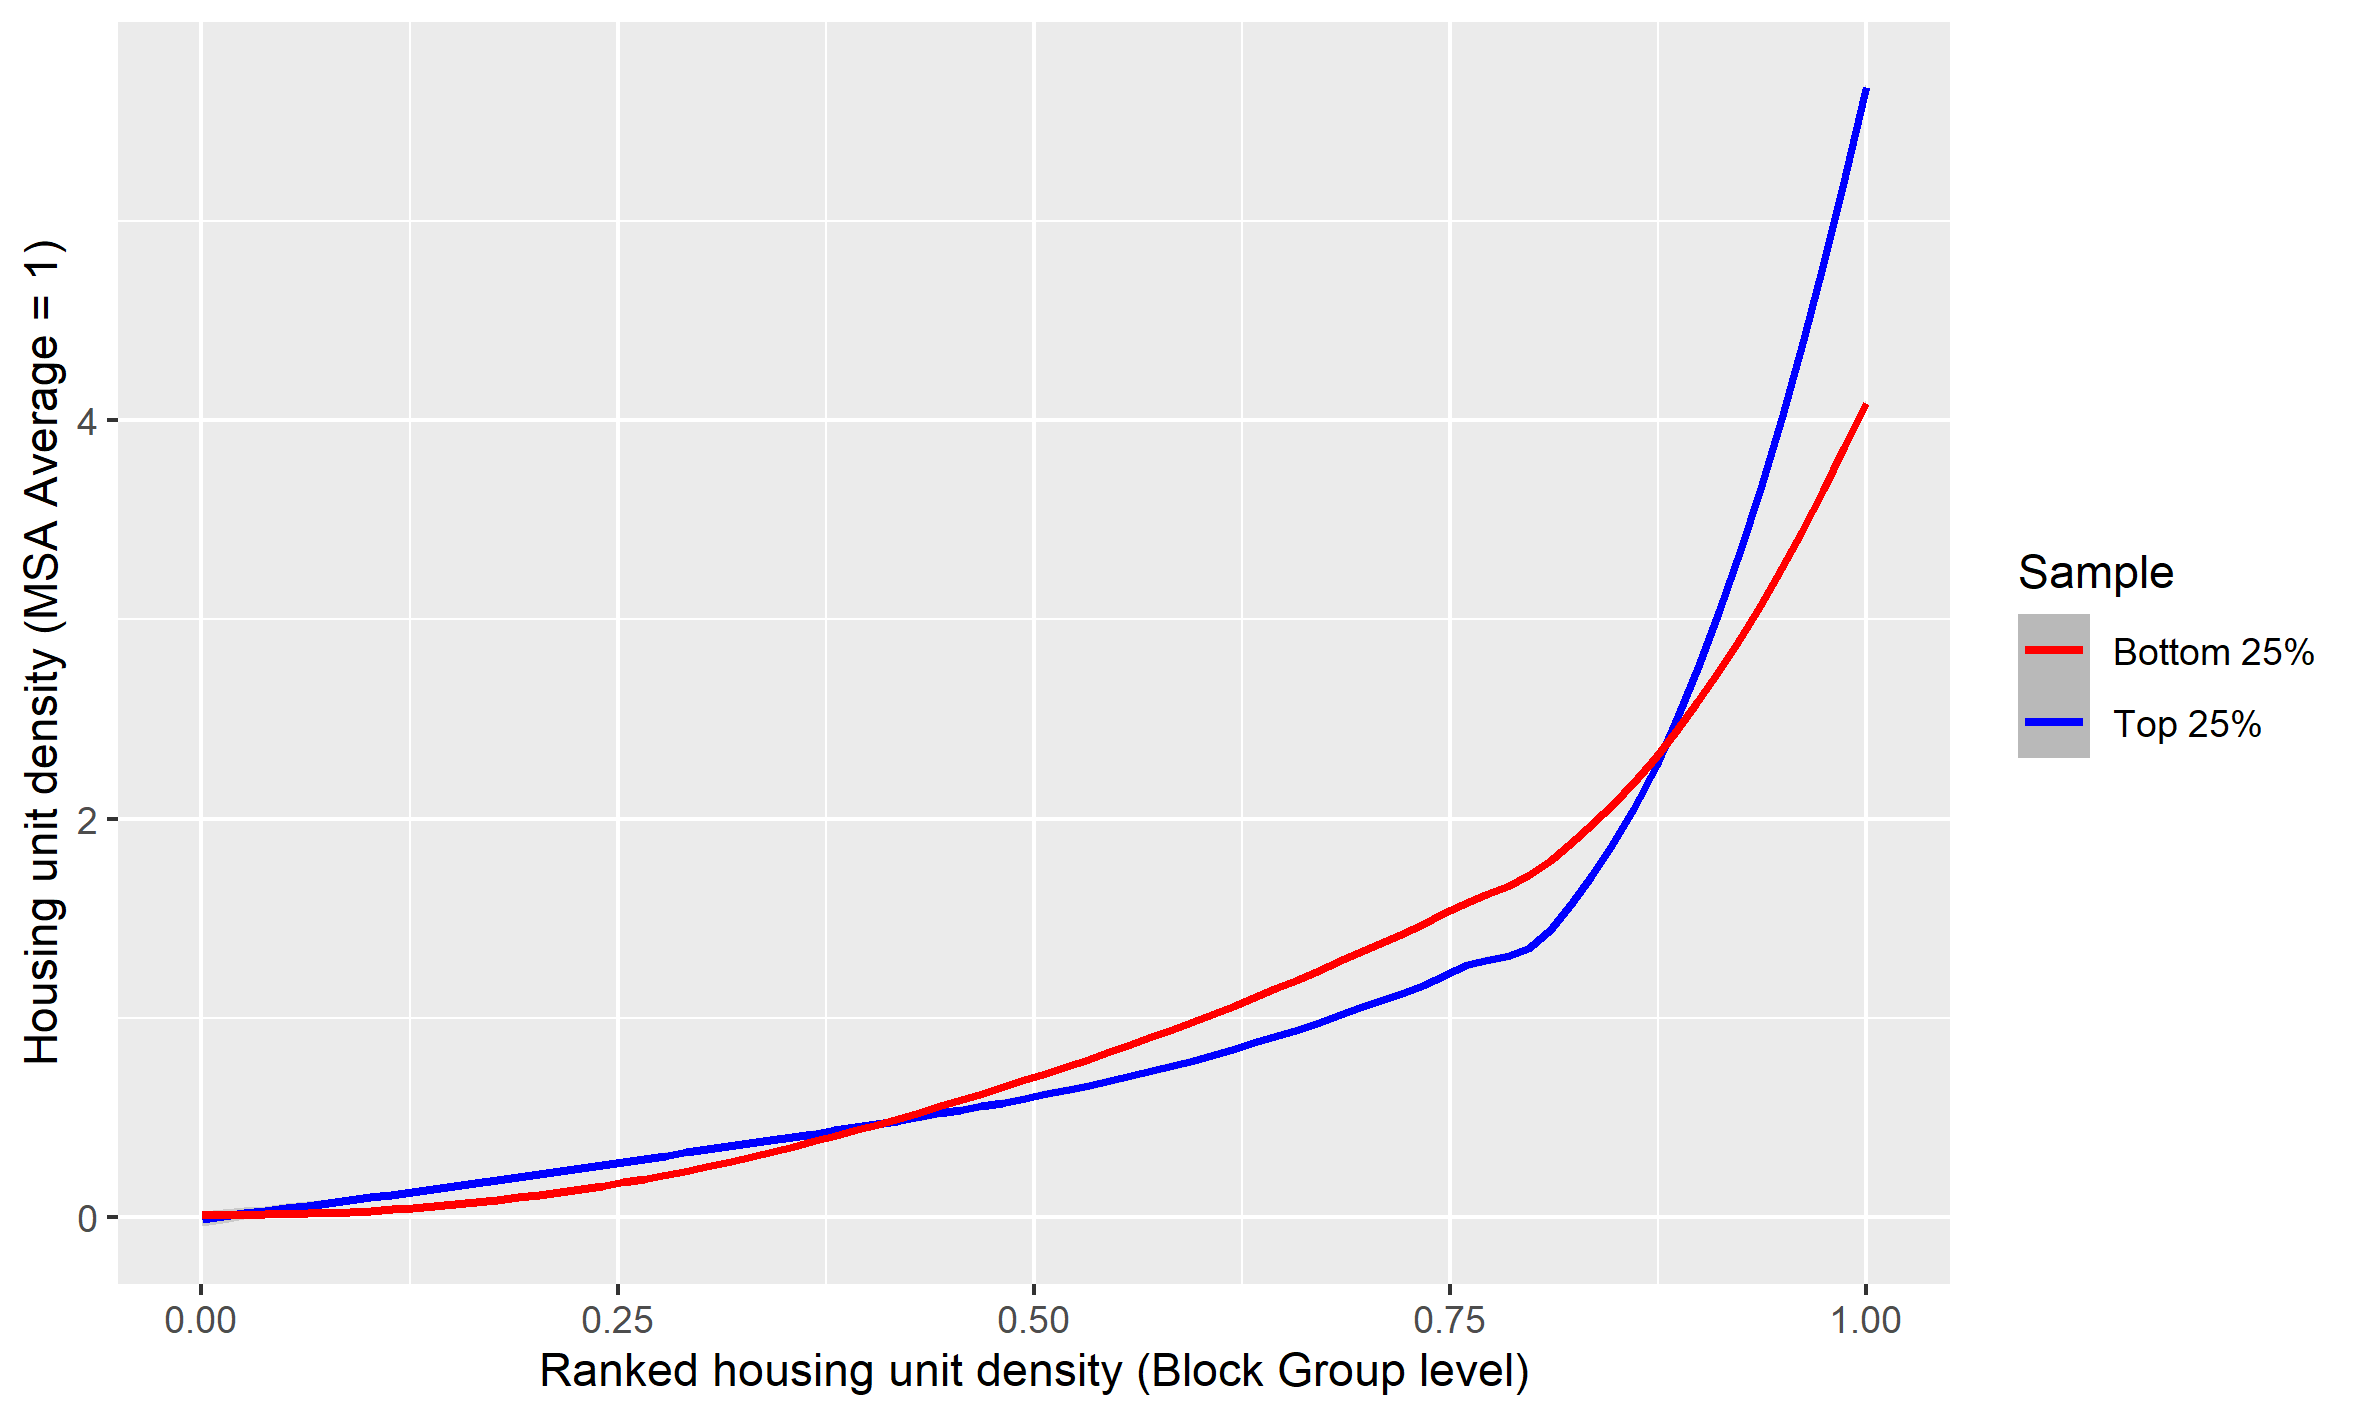
\includegraphics[width=1.1\textwidth]{blockdens_dist.png}
	\caption{Loess regression with $\alpha = 0.5$. 95\% confidence intervals are reported, but small enough to be hidden by the regression line. For the superstar sample, I take a random subset of the data to construct standard errors because of computational issues associated with Loess at large sample sizes.}\label{Blockdens_dist}
\end{center}
\end{figure}
\paragraph*{}
A roadblock in linking the patterns in Figure \ref{Blockdens_dist} to lot size regulation is that they may not be driven by the relative intensity of the development of structures associated with that regulation-- in particular, single family homes. To test this, I additively decompose housing unit density $H(i)$ in block group $i$ into two margins
\begin{equation}\label{SingleFMarginEq}
	H(i) = H_{Single Family}(i) + H_{Other Structures}(i)
\end{equation} 
where $H_{Single Family}(i)$ is the number of single family homes (detached and semi-detached) divided by the total land mass of the block group, and $H_{Other Structures}(i)$ is a residual\footnote{Recall that I demean average density by MSA to control for across-MSA variation in average density. Equation \eqref{SingleFMarginEq} still holds after this demeaning process. Moreover, the residual $H_{OtherStructures}(i)$ excludes boat and mobile homes.}. $H_{Single Family}(i)$ is inferred using the shares of housing units in single family homes from the 2008-2012 ACS combined with the 2010 census housing counts. I repeat the regressions in Figure \ref{Blockdens_dist} separately for both margins and report the results in Figure \ref{SingleFMargin} of Appendix \ref{DataandFactsContinued}. I find that the pattern of Figure \ref{Blockdens_dist} is driven entirely by the relatively low numbers of single family housing units per unit of land in the high density neighborhoods of expensive cities.
\paragraph*{}
With assessment data, I can probe this observation further. In fact, the pattern in Figure \ref{SingleFMargin} may be implicitly driven by two forces. On one hand, single family homes may actually be produced at low \textit{density}, hogging up space that could be used for other structures -- suggesting the importance of large lots. On the other hand, the low density of these units may be because they do not occupy much \textit{land}, which may suggest otherwise. To make this logic clear, I log-decompose the single family margin $H_{SingleFamily}(i)$ into a \textit{density} and \textit{land} margin, respectively
\begin{equation}\label{SingleFDensityMarginEq}
	\log(H_{SingleFamily}(i)) = \log(S_{Density}(i)) + \log(S_{Land}(i))  
\end{equation}
where $S_{Density}(i)$ is the \textit{inverse} average lot size of a single family home (under the assumption there is one Census household per single family home) and $S_{Land}(i)$ is the fraction of tract land used to produce single family homes. I measure $S_{Density}(i)$ using the average lot size of single family homes reported in the assessment files, and $S_{Land}(i)$ as a residual\footnote{Due to measurement error and incomplete coverage in the assessment files, the land share component has turned out to be larger than one for approximately 17,500 block groups of the over 175,000 in the MSA sample. I drop these observations only for the regressions of Figure \ref{SingleFDensityMargin}. Moreover, recall that $H_{SingleFamily}(i)$ carries a normalization factor when demeaning the density of housing units by MSA. I split this factor evenly across $S_{Density}(i)$ and $S_{Land}(i)$ in the regressions of Figure \ref{SingleFDensityMargin}.}. Like the previous exercise, I repeat the regressions of Figure \ref{Blockdens_dist} for each component in Equation \eqref{SingleFDensityMarginEq} separately, and report the results in Figure \ref{SingleFDensityMargin} of Appendix \ref{DataandFactsContinued}. I find that the differences in the density component $S_{Density}(i)$ between expensive and cheap cities is smaller in high density neighborhoods than in low density ones. In other words, the large lot sizes of single family homes can partially explain why we observe a relatively low density of housing units in the medium density neighborhoods of expensive cities.

\paragraph*{}
The nature and scope of land use regulation is thought to take on an entirely different form in European cities. As an additional robustness check, I test whether the results in Figure \ref{Blockdens_dist} hold in contemporary France -- and they do not. In doing so, I use OECD defined Functional Urban Areas (FUAs), microgeographic population distributions from the 2018 GEOSTAT data, and publicly available 2022 land value data from the Government of France. See Appendix \ref{FrenchDFC} for details on the construction of the data, and Figure \ref{Dens_dist_france} for the regression output. I also show that this result does not hold in the US historically using 1930 Census enumeration district data from the Urban Transition Project \citep{UrbTransitionProject}. See Appendix \ref{1930CensusDFC} for data construction details and Figure \ref{Dens_dist_1930ED} for output. 

\paragraph*{}
The collection of these observations is summarized in the following Fact:


\begin{theorem}\label{Fact1}
	Expensive cities appear to have a relatively smaller density of housing units in medium density neighborhoods. Likewise, high-density locations near downtowns and low-density locations on the urban fringe appear relatively more dense. This observation is in part driven by the relatively low density of single family homes, and does not appear to hold in contemporary France or in the early 20th century US. 
\end{theorem}

\paragraph*{}
Additionally, I show that  residential sorting on income underpins Fact \ref{Fact1}. There is a generally negative relationship between the rank of housing unit density and average income when considering variation strictly within cities. This observation has a rich history in urban economics, as has been previously attributed to the patterns of amenities \citep{parispoor} and income sorting into commuting \citep{ccpoortransport}. Moreover, I also find that income sorting on density is stronger in expensive cities in the sense that low density neighborhoods tend to be relatively higher income, and high density neighborhoods generally lower income\footnote{This holds true in all but the highest density neighborhoods (See Figure \ref{incomesorting}). Recent decades of gentrification may be leaving an imprint on the cross sectional data, and lot size regulation cannot explain gentrification.}. This harkens to a smaller literature on inequality and city size \citep{ineqcitysize} \citep{spatialsorting}, and the connection between city income inequality and income segregation \citep{FogliGuerrieri}. I argue that differences in the pattern of lot size regulation across samples play a role. To show these observations, I regress 2008-2012 ACS log average household income against the same ranking of housing unit density for each sample, and report both the regression and confidence intervals in Figure \ref{incomesorting}. Household income is demeaned by MSA to control for the urban wage premia. I summarize this observation in Fact \ref{Fact2}.

\begin{figure}[htbp]
	\begin{center}
		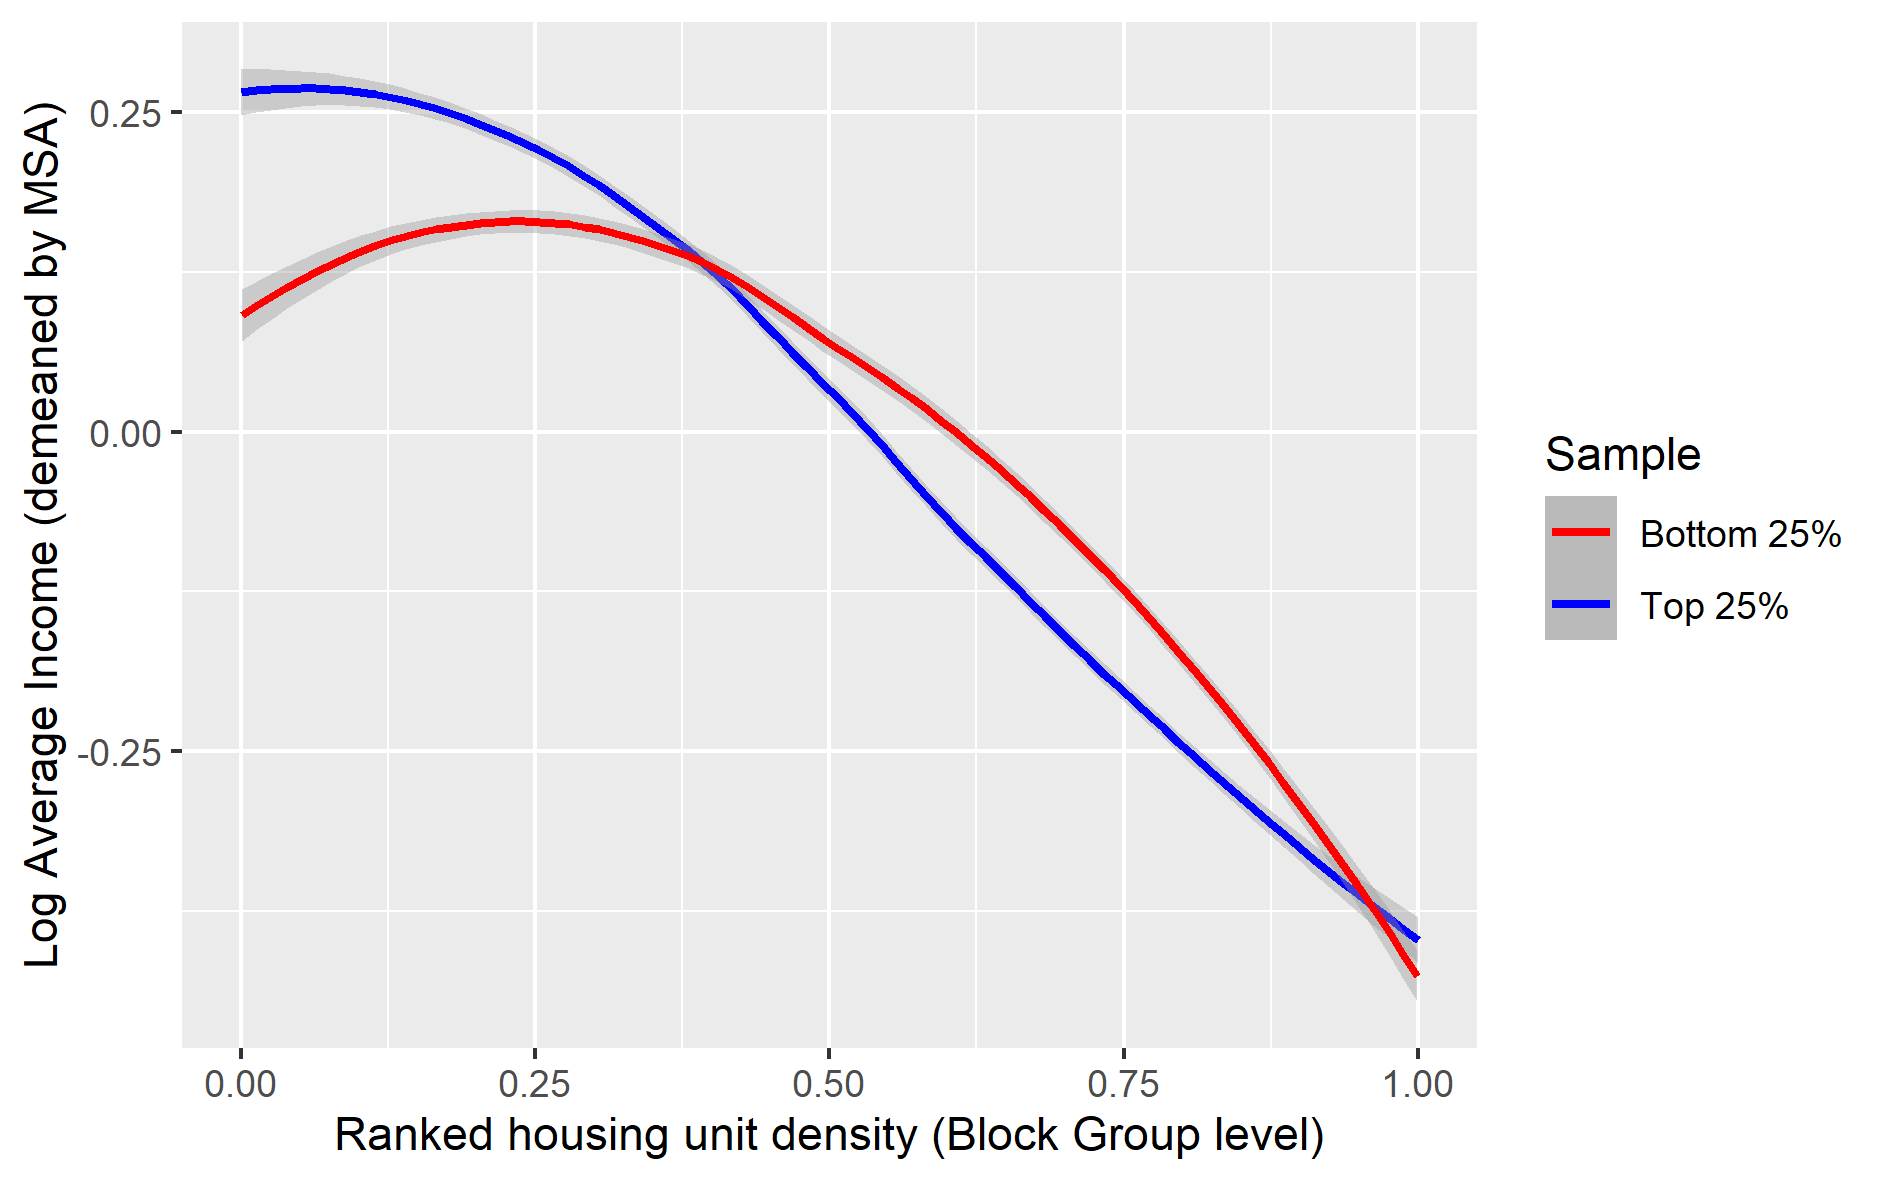
\includegraphics[width=1.1\textwidth]{income.png}
		\caption{Loess regression with $\alpha = 1$. 95\% confidence intervals are reported. For the superstar sample, I take a random subset of the data to construct standard errors because of computational issues associated with Loess at large sample sizes.}\label{incomesorting}
	\end{center}
\end{figure}


\begin{theorem}\label{Fact2}
	Within cities, there is a negative relationship between housing unit density and household income. This sorting pattern is relatively stronger in expensive cities.
\end{theorem}
\paragraph*{}
Facts \ref{Fact1} and \ref{Fact2} beg a question: can these observations be linked to more \textit{direct} measures of the stringency of lot size regulation? The model in Section \ref{section:Model} yields a simple way to measure lot size stringency from the assessment and transactions data. Suppose we have measured a minimum lot size $l(i)$ (in acres) in some census block group $i$, and suppose exactly one household must rent at least the amount of structure on that minimal lot to live in the neighborhood\footnote{In the model, I allow for duplexes, triplexes and fourplexes by making simple adjustments to the measured minimum lot sizes.}. Lastly, assume structure is supplied at a rate proportional to the size of the lot within a block group, and that the price for a unit of structure is uniform within a block group. Then, the value of the minimum amount of structure $I(i)$ is
\begin{equation}\label{observedStringency}
I(i) = V(i)l(i)
\end{equation}
where $V(i)$ is the value of housing per acre in $i$. Higher stringency levels imply stronger income sorting -- households with low income are forced to spend a large fraction of their income to rent the minimal lot. I measure $V(i)$ as the average value of of any home in the transactions data divided by the average lot size across single family homes, duplexes, triplexes and fourplexes. I go into great detail on how $l(i)$ is constructed in Section \ref{section:LotSizeMeasure}.
\paragraph*{}
Comparing within city variation of $I(i)$ between expensive and inexpensive cities reveals a single crossing pattern comparable to Figure \ref{incomesorting}. That is, high density neighborhoods in expensive cities appear to have a relatively lower stringency of regulation, and vice versa for low density neighborhoods. This can explain both facts in expensive cities: the relatively higher density and the relatively lower income in high density neighborhoods. I report this comparison in Figure \ref{stringencyPatterns}, following an similar procedure as above. Surprisingly, the results of this comparison are insensitive to the arbitrary choices of parameters used to construct $l(i)$; I elaborate in Section \ref{section:LotSizeMeasure}. 


\begin{figure}[htbp]
	\begin{center}
		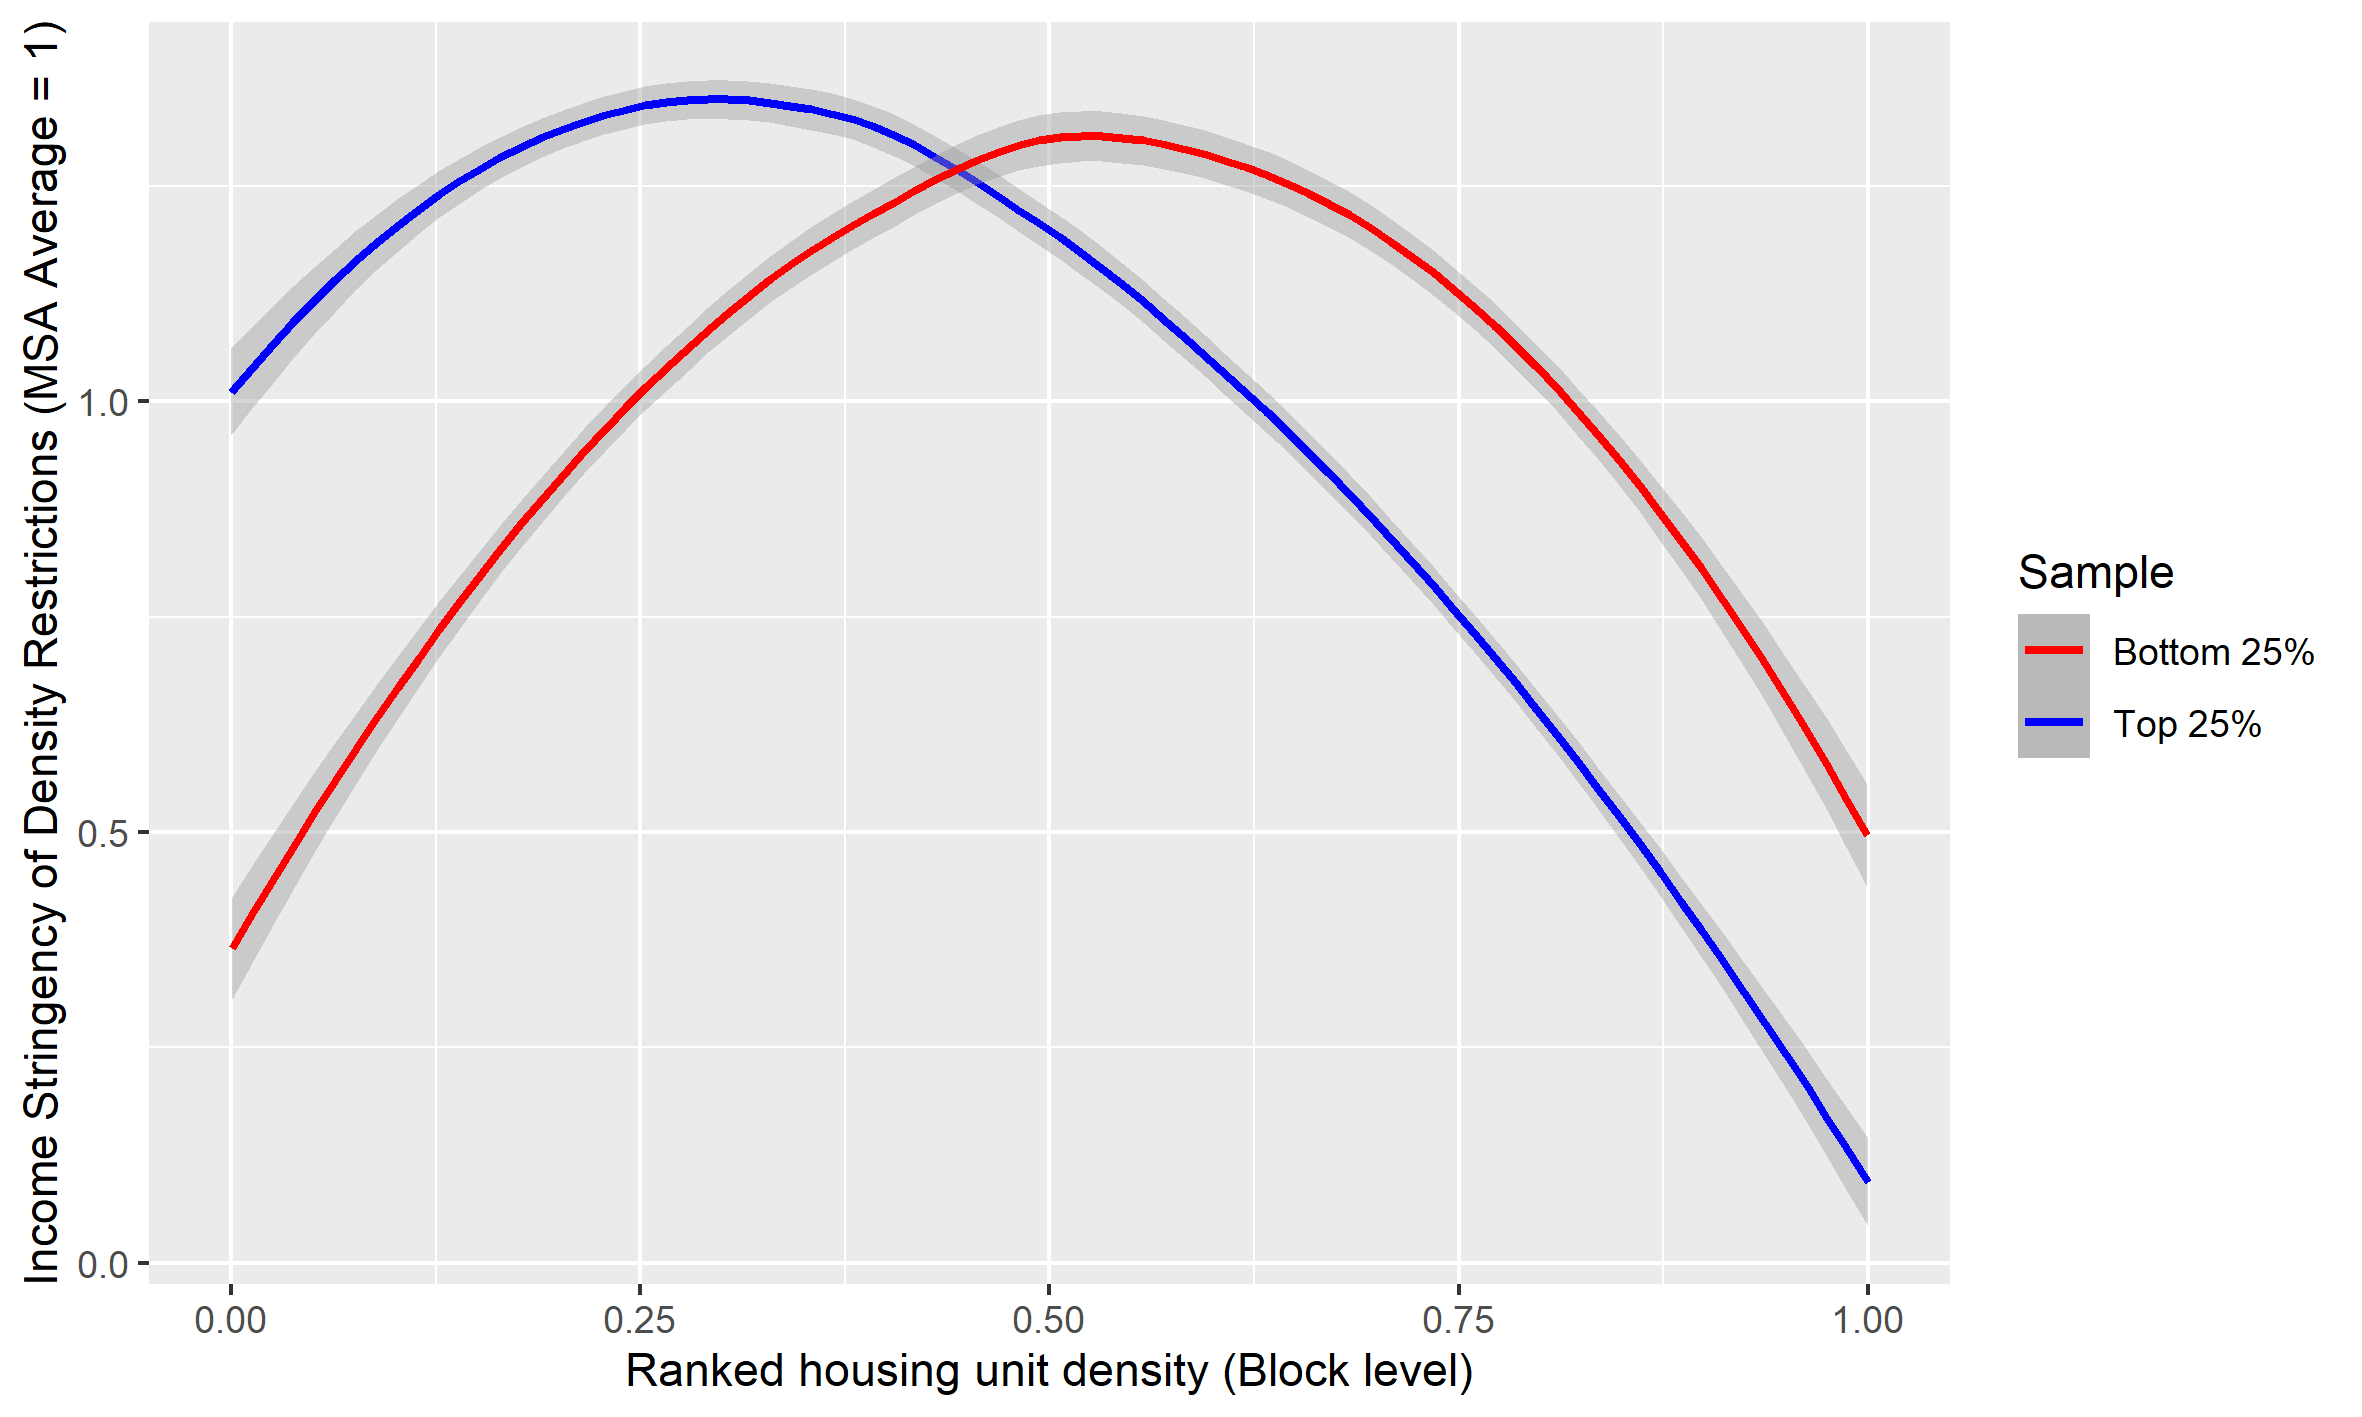
\includegraphics[width=1.1\textwidth]{stringencyofDensityRestrictions.png}
		\caption{Loess regression with $\alpha = 1$. 95\% confidence intervals are reported. For the superstar sample, I take a random subset of the data to construct standard errors because of computational issues associated with Loess at large sample sizes.}\label{stringencyPatterns}
	\end{center}
\end{figure}


\paragraph*{}
I will note here that counterfactual exercises in which lot sizes are eliminated show meaningfully different outcomes for the relationships in Figures \ref{Blockdens_dist} and \ref{incomesorting}. High density neighborhoods become significantly more affluent exclusively in expensive cities; severing the link between density and income sorting in them. Likewise, deviations in the housing unit density gradients between expensive and inexpensive cities also fall, corroborating the evidence in Fact \ref{Fact1}. 

\paragraph*{}
The variation in $I(i)$ \textit{across} cities also hints at a connection between lot size regulation and the urban wage premia. I find that the expensive cities have an average lot size stringency \textit{three times higher} than inexpensive ones. This forms an empirical basis for the importance of income sorting in mediating the effect of deregulation on aggregate labour productivity; and this is further corroborrated by the deregulation exercises in Section \ref{Section:Results}. I summarize these observations in Fact \ref{Fact3}.

\begin{theorem}\label{Fact3}
	Low density neighborhoods in expensive cities have a relatively higher stringency of lot size regulation. The opposite is true for high density neighborhoods. In addition, lot size stringency tends to be significantly greater in expensive cities. 
\end{theorem}


%%%%%%%%%%%%%%%%%%%%%%%%%%%%%%%%%%%%%%%%%%%%%%%%%%%%%%%%%%%%%%%%%%%%%
%%%%%%%%%%%%%%%%%%%%%%%%%SECTION THREE%%%%%%%%%%%%%%%%%%%%%%%%%%%%%%%
%%%%%%%%%%%%%%%%%%%%%%%%%%%%%%%%%%%%%%%%%%%%%%%%%%%%%%%%%%%%%%%%%%%%%
\section{Model}\label{section:Model}
\paragraph*{Geography}
I consider a finite set of cities $C$ indexed by $c$, which map to MSAs in the data. These cities are self-contained labour markets; that is, I do not allow households to access local technologies outside of the city for which they reside. Each city $c$ has an exogenous finite set of neighborhoods $N(c)$. I use the index $i$ to denote a typical neighborhood from any city, $i \in \cup_{c \in C}N(c)$, and define the map $C(i)$ to be the city associated with $i$. Here, neighborhoods are defined to be census block groups. Each of these neighborhoods have an exogenous amount of land $T_{R}(i)$ that is available to developers for the production of housing services.

\paragraph*{Developer's Problem}   
Complicating an otherwise standard specification of housing supply is the minimum lot size $\bar{l}(i)$ and the regulation of how many housing units can occupy each lot. To make the exposition clear, I start with preliminaries. In each neighborhood, I partition residential land $T_{R}(i)$ into equal sized \textit{parcels} of normalized mass $1$. That is, there are a mass $T_{R}(i)$ of parcels. These are the units of land that the representative developer uses to produce structure. These parcels can be \textit{split} into lots, and lots are a fundamental unit by which regulation operates. Each lot can hold a regulated maximum $\bar{h}(i)$ housing units. Only one household can occupy a housing unit. For example, $i$ may allow duplexes, so that $\bar{h}(i) = 2$. Then, $\bar{l}(i)/\bar{h}(i)$ is the minimum amount of land per housing unit in $i$. Let $l(i)$ denote this minimum land per housing unit, which will be the main object I work with hereafter\footnote{I'm making a very implicit assumption here, i.e. there is no material difference between single family homes on small lots or multifamily homes on large lots.}. Of course, $l(i)$ may be zero if the neighborhood is unregulated. 
\paragraph*{}
Given a parcel in $i$, developers choose the total amount of structure $A(i)$ that can occupy it in a standard way. That is, they use a neighborhood-varying Cobb-Douglas technology over land and capital, facing a perfectly elastic supply of that capital at rate $r$. This yields the neighborhood-level housing supply function per unit of land
\begin{equation}\label{supplyfn}
	A(i) = \lambda(i)P(i)^{\epsilon(i)}
\end{equation}
where $P(i)$ is the price of an effective unit of housing stock, $\epsilon(i)$ is the supply elasticity in block group $i$ and $\lambda(i)$ is a supply shifter net of capital costs. In a world without minimum lot sizes, the developer is indifferent to allocating this structure across housing units; there can be many small houses or few large ones, provided the total stock is given by \eqref{supplyfn}. Instead, if developers respect the minimum lot size, the minimum amount of housing stock per housing unit $A^{\star}(i)$ must be

\begin{equation}\label{minstructure}
	A^{\star}(i) = \lambda(i)P(i)^{\epsilon(i)}l(i)
\end{equation}

\paragraph*{}
Equation \eqref{minstructure} reveals the material difference between lot size regulation and other regulations studied in contemporary quantitative models. Contrast the equation with the standard Floor Area Ratio restriction in \cite{bruecknersingh} or \cite{BruecknerFuGu}, which puts limits on housing \textit{stock} per parcel. Here, there are no stock density  limits -- just limits on the number of housing units (or households) that can occupy a parcel. This distinction is forcefully argued in \cite{griesonwhite}.

\paragraph*{}
Equation \eqref{minstructure} also reveals how minimum lot sizes and housing unit density restrictions cause income sorting. I take the quantity $A^{\star}(i)$ as a minimum amount of housing stock required to be purchased to live in neighborhood $i$; households with income below $P(i)A^{\star}(i)$ will be priced out of the local housing market. This quantity is increasing in housing prices, holding regulation fixed. Moreover, households with little disposable income after paying for this minimum quantity are forced to purchase more than what they would if this quantity could be freely chosen. This feature does not exist in a recent generation of urban models that study stock density restrictions, such as \cite{acosta}, \cite{martynov} and \cite{anagoletal2021}. 

\paragraph*{Consumer's Problem}
Households have Cobb-Douglas preferences over a freely traded, homogenous good $g$ (with a normalized price of 1 dollar) and housing $A$. Households differ along two dimensions. The first is by \textit{education}; whether a household head holds at least a college degree, indexed by $s \in S$. The second is by \textit{skill}, or units of effective labour, indexed by $f$ and lying in a finite support $F$. Henceforth, I denote $z$ as the index of the pair $(s, f)$, let $s(z)$ and $f(z)$ be the education and skill levels associated with $z$, and define $Z := S \times F$ to be the space of household types. 
\paragraph*{}
Let $\bar{L}(z)$ be the mass of type $z$ households. Deferring neighborhood choice for a moment, suppose a household of type $z$ has chosen $i$.  Given the city $C(i)$ and education $s(z)$ associated with the household and its location, it receives a wage $w_{s(z)}(C(i)) := w_{s(z)}(i)$ per effective unit. Given this wage, the household of type $z$ solves
\begin{equation}\label{utility}
	\max_{A, g} A^{\beta}g^{1-\beta}
\end{equation} 
subject to $A \geq A^{\star}(i)$ and $P(i)A + g \leq w_{s(z)}(i)f(z)$. Let  $V\big(P(i), f(z), w_{s(z)}(i), A^{\star}(i)\big) : = V(i, z)$ be the solution to Equation \eqref{utility}, which implicitly depends on prices, wages and other endogenous variables. If the price of a minimally sized lot exceeds income at $z$, I set the utility of consumption to be zero and assume that household spends all their income on housing.

\paragraph*{Neighborhood Choice} 
Apart from consumption of housing and other goods, each neighborhood $i$ provides an \textit{amenity value} $b(i, z)$ for households of type $z$. Households also draw idiosyncratic amenities shocks over neighborhoods. These shocks are distributed multivariate Gumbel, yielding a nested logit model. The mass of $z$ households who choose neighborhood $i$ is 
\begin{equation}\label{laboursupply}
	L(i, z) = \bigg[\frac{e^{\theta(z) W(C(i), z)}}{e^{\boldsymbol{W}(z)}}\bigg]\bigg[\frac{b(i, z)e^{\rho(z) V(i, z)}}{e^{W(C(i), z)}}\bigg]\bar{L}(z)
\end{equation}
 where 
 \begin{equation}
 	W(C(i), z) = \log\bigg[\sum_{i' \in N(C(i))}b(i', z)e^{\rho(z) V(i', z)}\bigg]
 \end{equation} 
is the expected welfare of a household $z$ who chose a neighborhood in $C(i)$ and 
\begin{equation}\label{expwelfare}
\boldsymbol{W}(z) = \log\bigg[\sum_{c \in C} e^{\theta(z) W(c, z)}\bigg]
\end{equation}
is the expected welfare of a type $z$ household before drawing a shock. This is our standard measure of welfare moving forward. $\theta(z)$ governs how responsive migration flows are across cities to changes in the consumption value of a neighborhood in the city. $\rho(z)$ governs the responsiveness of migration flows within cities with respect to values of individual neighborhoods; both semi-elasticities are allowed to vary by type. If $\rho \to \infty$ and $\theta \to \infty$, we are essentially in a open city model with perfect mobility. Likewise, if $\theta \to 0$ with $\rho \to \infty$, we are in a closed city model. Separating the migration elasticity in this way is motivated by the variation in the stringency of density restrictions, both within and across cities. In other words, the model doesn't take a stand on how easy it is for a low income household to move downtown to escape large lots, or to move to a less expensive city entirely.  

 
\paragraph*{}
Before continuing, I note two caveats inherent in the choice model. Firstly, allowing amenity values $b(i, z)$ to vary as flexibly as possible by socioeconomic status is crucial for explaining the observed residential sorting on income. However, I do not observe the joint distribution of neighborhood, income and education status within cities, so I make some lax restrictions on these amenities. I elaborate in Section \ref{section:CalibrationIdent}. Secondly, the structure of the choice model allows for households who cannot afford the pay for a house on a minimal lot to live there. This feature grapples with the reality that the types of households whom the model predicts would be priced out of the housing market actually show up in observation. This can be for many reasons, including model mispecification, unobserved wealth (especially housing wealth) and unobserved permanent income.

 \paragraph*{Endogenous Amenities} 
 The income sorting caused by the regulation may have important implications for shaping the spatial pattern of the amenity values $b(i, z)$. Before delving into the microfoundations of these spatial patterns, I specify a relation determining the amenity in my baseline model:
 \begin{equation}\label{endoamen}
 	\log\big[b(i, z)\big] = -\kappa\tau(i) + \Omega\log\bigg[\frac{\sum_{z' \in Z}w_{s(z')}(i)f(z')L(i, z')}{\sum_{z' \in Z}L(i, z')}\bigg] + \epsilon(i, z)
 \end{equation}
 where $\tau(i)$ is the average neighborhood commute time, the second term is income per capita of neighborhood $i$ and $\epsilon(i, z)$ are exogenous residuals. 
 \paragraph*{}
 There are at least two main channels that I have emphasized thus far that would proximally give rise to \eqref{endoamen}. Firstly, local income could increase local amenities through variety effects in a Dixit-Stigliz style model \citep{AlmagroDI} \citep{Coutureetal}, while local population could decrease the amenity value through urban congestion effects or from the disutility of density highlighted in \citep{KSC}. When these two forces operate at the same elasticity $\Omega$, amenity values depend only on income per capita. Secondly, local governments could provide a congested public good financed through property taxes \citep{calabresetal}. In that case, income per capita would be replaced with property tax revenue per capita. In a model with Cobb-Douglas preferences, no lot sizes and random heterogeneity in property tax rates, this is almost identical to income per capita. With assessment data, I have the luxury of playing around with different specifications as a substitute for model selection. These alternatives will be considered in future drafts. 
 
\paragraph*{}
However, I do not want to limit myself to these interpretations. Instead, I assume $\Omega$ includes all factors that could be \textit{caused} by income per capita. Apart from the above, these may include reduced crime or other types of peer effects. 
 
\paragraph*{Production} In each city $c$, production of the numeraire good $g$ takes place at a central business district using a CES technology over workers of differing education levels

\begin{equation}\label{production}
g(c) = \bigg[\sum_{s \in S}\Sigma(c, s)^{\frac{\sigma - 1}{\sigma}}D(c, s)^{\frac{\sigma - 1}{\sigma}}\bigg]^{\frac{\sigma}{\sigma - 1}}
\end{equation}
 where $\Sigma(c, s)$ is a city productivity for type $s$ workers and $D(c, s)$ is the level of employment\footnote{I adopt this monocentric production model because of data limitations. The model would otherwise predict income sorting into commuting because lot sizes may be more stringent away from employment centers, as I claim from the observational evidence. In a polycentric world with varying within-city productivity, one would require household level commuting data to parse the selection bias when calibrating this productivity.}. $\Sigma$ is taken as exogenous with respect to firm employment descisions, but is allowed to vary by city population with elasticity $\alpha$
 \begin{equation}
 	\Sigma(c, s) = \omega(c, s)\bigg[\sum_{z \in Z, i \in N(c)}L(i, z)\bigg]^{\alpha}
 \end{equation}
 for exogenous $\omega(c, s)$. 
 
 \paragraph*{Endowments} Land is owned by a set of spatially immobile landlords who do not consume housing, which follows from a long tradition in Alonso-Muth-Mills style models \citep{bruecknerhandbook}. However, welfare calculations ideally take into account the joint distribution of household types, neighborhoods and home-ownership rates. For example, high income households may be hurt when loosening lot size requirements both through their direct consumption of the neighborhood amenity and through rents on land they do not consume. This has been shown to be consequential in structural models featuring regulation, including \cite{parkho}. I do not observe this distribution, and instead consider welfare separately as if they were two distinct groups. 
 
 
 \paragraph*{Equilibrium} An equilibrium is defined as a set of housing prices $P(i)$, wages $w(c)$, neighborhood allocations $L(i, z)$, amenities $b(i, z)$ and minimum structure requirements $A^{\star}(i)$ such that 
 \begin{enumerate}
 	\item Labour Markets clear: Given indirect utility $V\big(P(i), z, w(c), A^{\star}(i)\big) : = V(i, z)$ solving \eqref{utility}, amenities $b(i, z)$ solving \eqref{endoamen} and labour supply per household type $L(i, z)$ solving \eqref{laboursupply}, we have $\sum_{i \in N(c)}\sum_{f \in F}fL[i, \small(s, f\small)]$ equals labour demand for each education level $s$ derived from \eqref{production} in every city $c$.
 	
 	\item Housing Markets clear: Given $A^{\star}(i)$ solving \eqref{minstructure} and population $L(i, z)$, the neighborhood demand for housing stock derived from \eqref{utility} equals the neighborhood supply of housing stock derived from \eqref{supplyfn} in every $i$. 
 \end{enumerate}




%%%%%%%%%%%%%%%SECTION: MEASURING LOT SIZES%%%%%%%%%%%%%%%%%%%
\section{Measuring Lot Sizes}\label{section:LotSizeMeasure}
\paragraph*{}
 If the distribution of household incomes is granular in a neighborhood, the model implies that there is a "bunching" of lot sizes around the regulatory minimum $l(i)$. Exploiting this idea, \cite{Song} demonstrates that measuring discontinuities or "structural breaks" in the distribution of local lot sizes works well to identify these regulations. One issue faced in the paper is how to define "local" -- a geographic region by which to run this algorithm. The issue is that regulation varies widely at the microgeographic level, but one needs a sufficient amount of data both below and above the regulatory minimum to rule out spurious discontinuities. In other words, conditional on identifying a correct regulatory boundary, one wants to use as much data in that boundary. Since my model is aggregated from the household level to the block group level (which tend to be smaller than the spatial units in which general zoning rules are assigned), I use a clustering algorithm on census block groups to define these local Zoning Districts. This approach is taken by \cite{Song} in scenarios where data on zoning rules at the lot level are missing. 

\paragraph*{Defining Zoning Districts} For the purposes of this draft, I do not use direct observations of zoning rules in the assessment files to cluster block groups into these zoning districts\footnote{Incorporating these data would have required a reconstruction of the Zillow data provided to me. Since I will need to reconstruct the CoreLogic data anyways, I thought that my time would better be spent actually coding up a model and thinking about the results for the August presentation. This turns out to have been crucial for getting the results and a draft in time.}. Instead, I cluster along a host of dimensions, including shares of land use single family homes and multifamily homes (and the modes and quartiles of their lot size distributions), as well as shares of land designated commercial and vacant. Missing data in any of these categories are imputed as 0 strictly for the purposes of the clustering. To consider the spatial cohesion of these groups, I employ the algorithm of \cite{Chavent2018} which allows one to weigh the importance of geographic proximity in the assignment of clusters. I target the number of block groups in each zoning district to be ten on average; roughly the size of three census tracts\footnote{This target is implemented as follows: within each MSA, I assign a minimum number of clusters equal to the number of block groups divided by ten (rounded to the nearest integer), and allow the maximum number of clusters to equal the number of block groups. I then select the desired number of clusters within this range using the Silhouette score, which is a standard statistic in the clustering literature. This process clusters roughly 174,000 block groups into 20,000 zoning districts.}. Figure \ref{ZoningDistrict} of Appendix \ref{appendix:LotSize} shows the 41 zoning districts assigned in San Francisco county. The algorithm is able to distinguish single family neighborhoods in the south and southwest from the central business district in the northeast. 

\paragraph*{Measuring Structural Breaks} Armed with these zoning districts, I measure the "bunching" of lot sizes as the smallest mode of the distribution of lot sizes within them\footnote{\cite{Song} uses an MSE loss function to measure these discontinuities. Frankly, my implementation of this loss function yielded substandard estimates when compared to the mode.}. I also generalize this measurement beyond single family homes to duplexes, triplexes and fourplexes. To do so, I scale the distribution of lots under these different structures by the implicitly allowed units per lot and solve for the mode of each of those distributions separately. I limit the sample of assessments to the most recent in 2015, and the same sample is used to construct the variables used in clustering.

\paragraph*{Additional Cleaning}
There are three large issues with interpreting these measurements as regulation. Firstly, my model intentionally includes neighborhoods in downtowns where unit density restrictions don't officially exist. For example, suppose we observed some "minimum lot size" in a neighborhood with a set of single family homes, but also a large amount of land zoned for large apartments. From the census, we would observe considerably more housing units in this neighborhood than what would be implied by the inferred regulation and a measurement of total residential land use. Secondly, the official minimum lot size may differ strongly from the actual dimensions of regulated structures that exist. These cases would depend in an ad-hoc way on how lienient the local government is when granting permission for zoning variance, or on how many homes exist that predate the regulation. Thirdly, the mode does a very bad job of measuring regulation in remote locations that tend to have massive lots (greater than 5 acres). I detail a procedure on how I correct for these cases and assign a final density restriction $l(i)$ to use in calibration.
\begin{enumerate}
	\item First, I define a "Restriction Threshold" $U_{1}$ lying in the unit interval. If the fraction of lots with sizes below the measured mode are above this threshold for any structure type (single family, duplex, etc.), I assign an $l(i)$ of zero. For duplexes, triplexes and fourplexes, I drop the corresponding mode measurements if the fraction of housing units in those structures (from the 2008-2012 ACS) are below some "Mode Threshold" $U_{2}$, provided a mode from another structure type could be measured.
	
	\item I take the minimum of the leftover modes across structure types as a single measurement to be passed for further cleaning. 
	
	\item I assign an $l(i)$ of zero to block groups that have the number of 2010 Census housing units above what would be implied by the measured mode and some measure of total residential land use $T_{R}(i)$. To construct $T_{R}(i)$, I first measure what the total lot area would be if all Census homes were in a regulated structure (single family to fourplex) by multiplying the average adjusted lot size from the assessments by the Census household counts in each neighborhood. In a minority of neighborhoods, this total lot area exceeds the known land mass of the block group (due to measurement error), so I set $T_{R}(i)$ to be the minimum of these. Note that the potential overestimation of $T_{R}(i)$ in unregulated neighborhoods is inconsequential for equilibrium outcomes because the supply shifter $\lambda(i)$ can be arbitrarily chosen to clear markets -- see Equation \ref{supplyfn}. 
	
	\item For any measured mode above 5 acres, I reassign the lot size restriction to 5 acres. This corresponds to roughly 400 block groups out of the 171,000 in the final sample. Little is known about the largest minimum lot size requirement in the United States -- so this is a bit ad-hoc. 
	
	\item I set $l(i)$ to $0$ if no mode from any structure type can be assigned to a neighborhood in the sample. 
\end{enumerate}

\paragraph*{}	
Below, I report the final distribution under the parameters $U_{1} = U_{2} = 0.35$. The relationships in Fact \ref{Fact3} appear to be  invariant to choice of these parameters and the top-coding threshold for lot sizes. Figure \ref{regHistogram} reports the histogram of the final assigned density restrictions $l(i)$. 60,000 of the 171,000 block groups are assigned no density restriction. 

\begin{figure}[hbpt]
	\begin{center}
		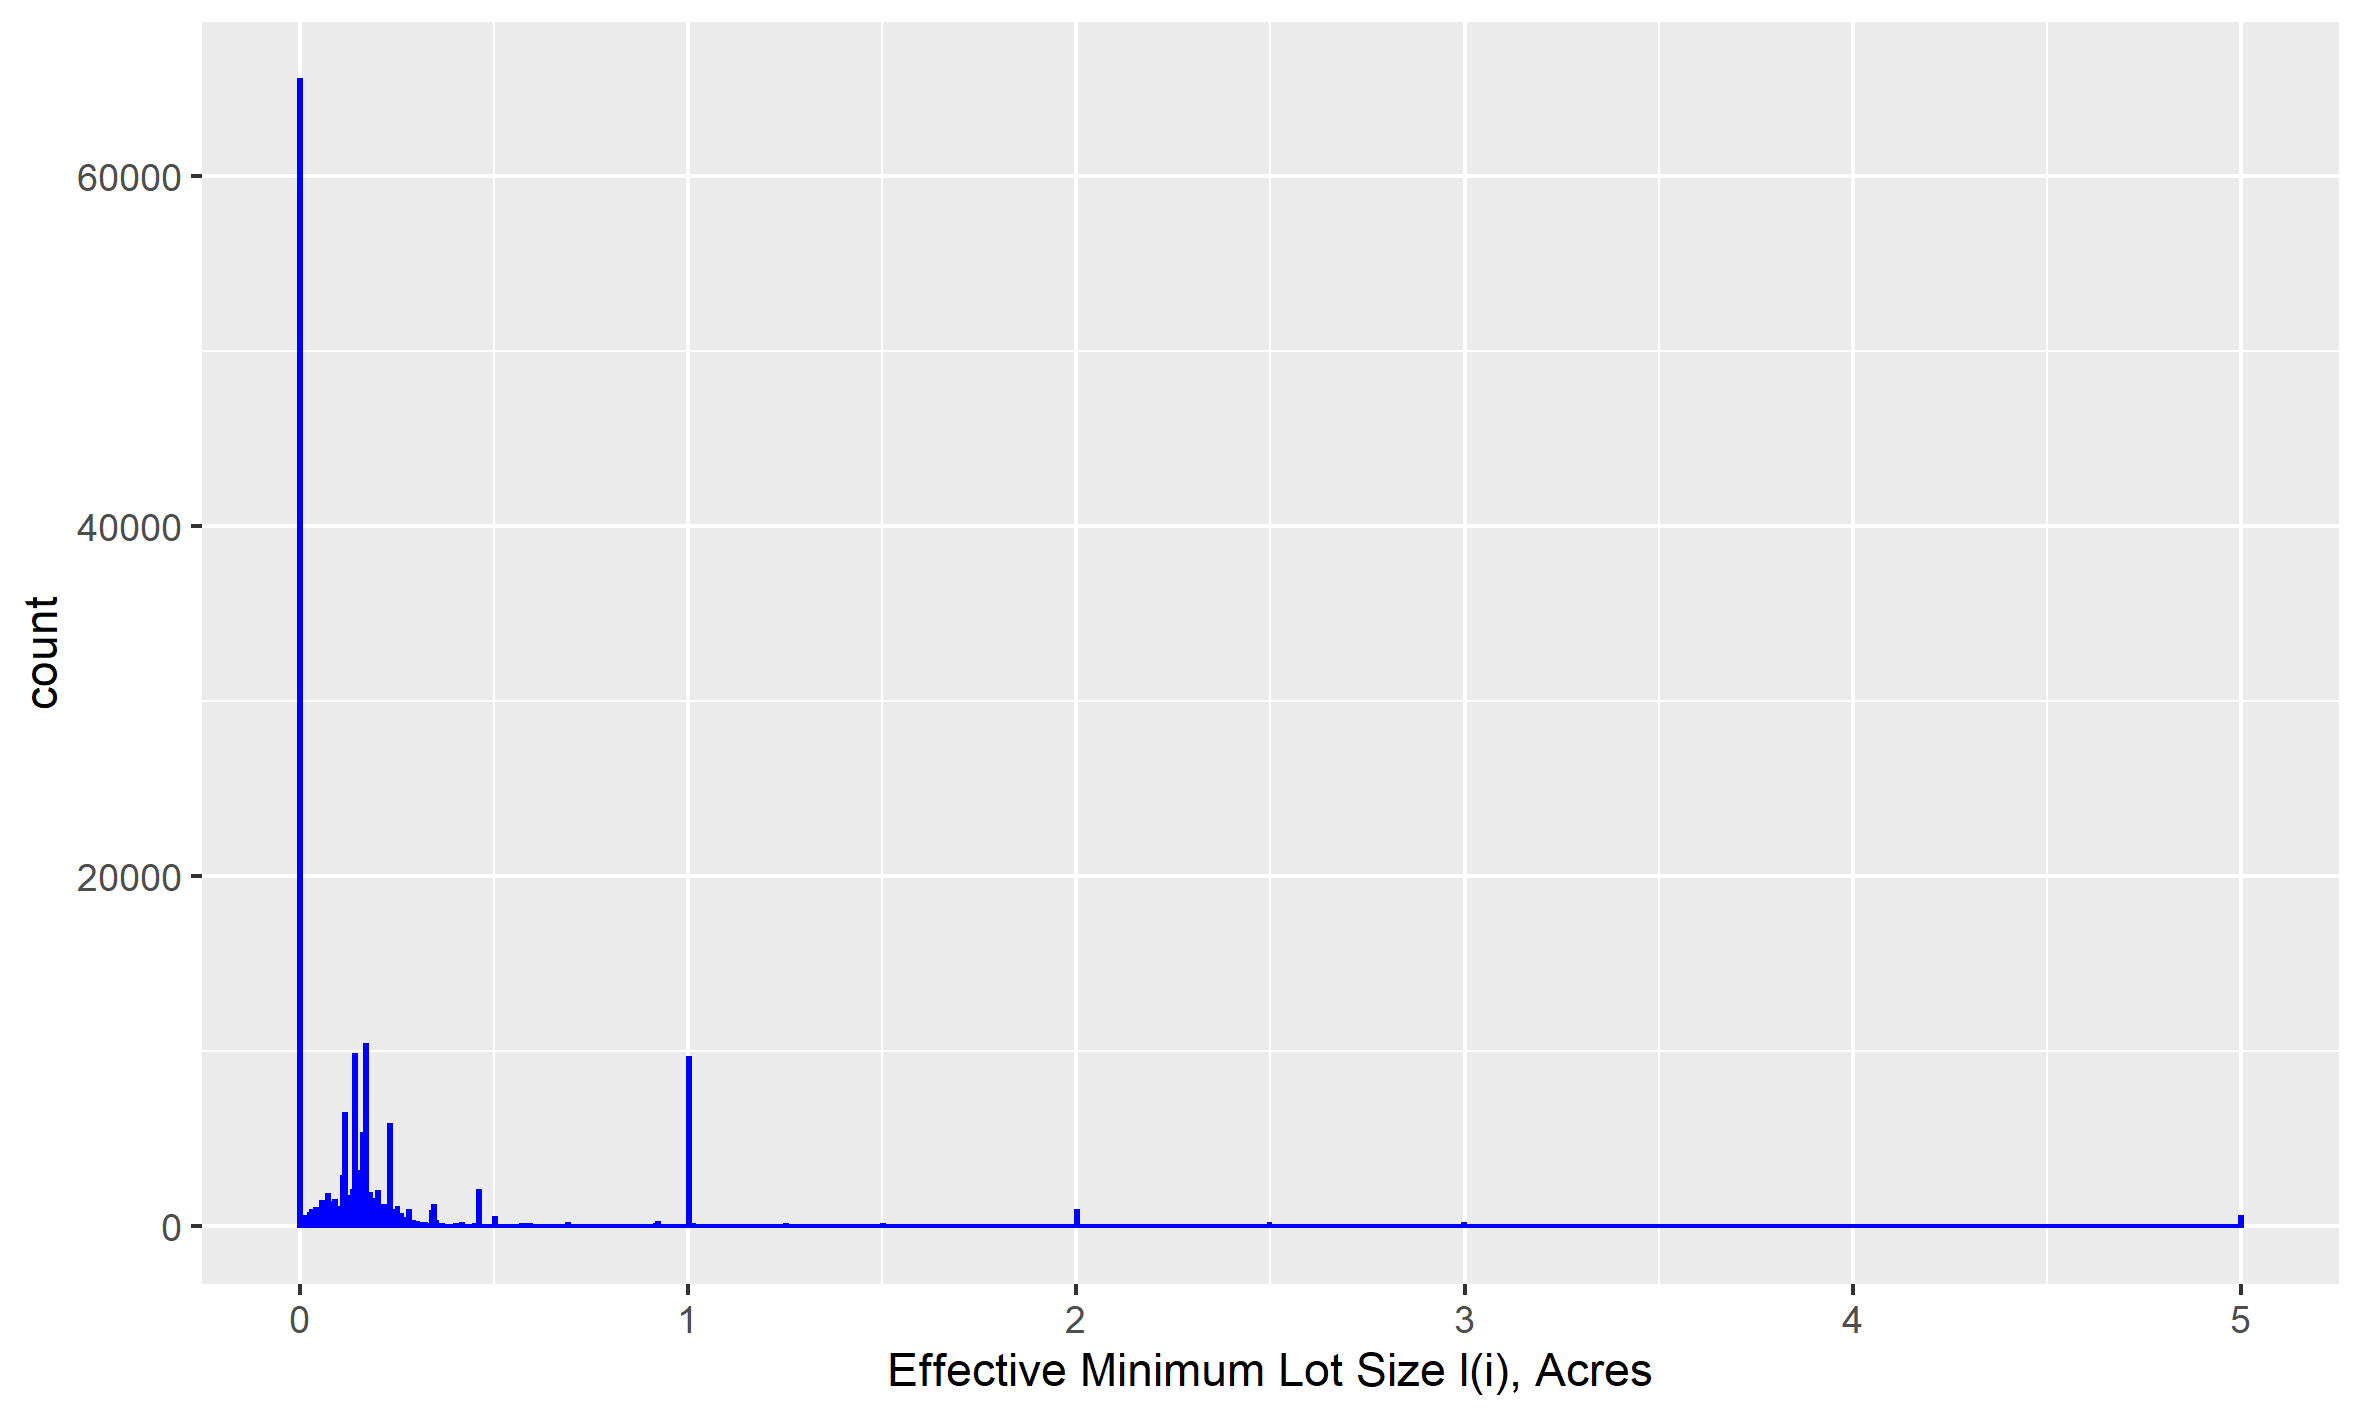
\includegraphics[width=\textwidth]{DistDensRegulation.png}
		
		\caption{Histogram of (effective) density restrictions used in the model.}\label{regHistogram}
	\end{center}
\end{figure}



%%%%%%%%%%%%%%%%%%%%SECTION  CALIBRATION%%%%%%%%%%%%%%%%%%%%%%%%%%%%%%%%

\section{Calibration and Identification}\label{section:CalibrationIdent}

\paragraph*{}
In this section, I sketch a procedure that estimates some parameters and chooses others to rationalize the data as an equilibrium of the model.

\paragraph*{Housing prices} The value of a house is determined by both its underlying quality and the price paid for that quality. Assessment data are detailed enough to allow unit prices $P(i)$ to be parsed from observed housing characteristics that determine quality. Following \cite{BSH}, I construct them using the following hedonic regression
\begin{equation}
	\log[Value_{iht}] = \log[P(i)] + Controls_{iht} + \sum_{t \in Year}FE_{t} + \sum_{t \in Month}FE_{t}
\end{equation} 
where $Value_{iht}$ is the observed transaction value of the house $h$ at time $t$, $Controls_{iht}$ are a set of observed characteristics, $FE_{t}$ are year and month fixed effects in the 2008-2012 sample of housing transactions linked to the 2015 current assessments. Identification of housing prices $P(i)$ are from block group fixed effects. Controls include the type of structure (single family, apartment), floorspace, lot size, number of rooms, bathrooms, types of AC and heating systems, roof and foundation types, sewage systems, and more characteristics recorded to assess the value of the house. 
\paragraph*{}
A considerable number of housing transactions appear unrealistically small -- suggesting the presence of non-market transfers. I drop transactions that are recorded not at arms-length and below the bottom 1\% of self-reported housing values in each MSA from the 2008-2012 ACS. This adjustment removes approximately 5\% of transactions included in the period. I also drop transactions in the top 0.1\% of these self reported housing values in each MSA, which accounts for clear outliers in block groups where there aren't many recorded transactions used to construct the fixed effect.  
\paragraph*{}
This procedure yields prices for approximately $140,000$ block groups out of the $171,000$ in the final sample. To increase coverage, I follow \cite{BSH} and construct lower-quality indices using the 2008-2012 ACS. To ensure that these prices are of similar scale, I adjust the ACS derived prices in each of the $171,000$ block groups so that the log mean and variance are identical to the $140,000$ assessment-based prices. I use the derived ACS prices in cases where the assessment prices are missing, and drop approximately $2,500$ block groups from the full sample where both are missing. 

\paragraph*{City productivity} Central to the model is the potential for city sorting on household characteristics correlated with income and education. As a result, wage differentials across cities may be larger than what would be suggested in a Rosen-Roback spatial equilibrium. To measure wages in terms of efficiency units of labour, I follow \cite{ineqincreased} and regress log hourly wages in a set of occupation, sex, race, ancestry, year, quadratic in age and years of education, including MSA fixed effects using the 2008-2012 ACS individual sample\footnote{Households in approximately 80 2013-definition MSAs cannot be directly identified in the 2008-2012 IPUMS ACS sample. For these MSAs, I use the official IPUMS PUMA-MSA crosswalk, matching PUMAs to MSAs based on the largest land coverage.}. I define education groups by whether an individual holds a 4 year college degree, and run this regression separately by group. The MSA
fixed effects in this regressions define the education-city wages $w_{s}(c)$. I normalize $w_{s}(c)$ so that it is on average one across cities for each education level, noting that the relevant interpretation of household efficiency units $f$ is then the total labour income that can be earned in an average city. Productivity $\Sigma(c, s)$ can then be inferred on a inversion of the producers problem associated with Equation \eqref{production} after measuring total labour supply by education and MSA. 

\paragraph*{Local household type distributions} Calibrating underlying amenity values $b(i, z)$ requires constructing measures of the local mass of households by type $L(i, z)$. The 2008-2012 ACS reports yearly household income distributions at the block group level aggregated to 17 income bins. To alleviate issues associated with model granularity as in \cite{DingelTintelnot:2021}, I aggregate these bins further into 7; reducing the space of types $Z$ to a size of 14\footnote{These income bins are (in yearly household income) $\$0-25,000$, $\$25,000-50,000$, $\$50,000-75,000$, $\$75,000-100,000$, $\$100,000-150,000$, $\$150,000-200,000$ and $\$200,000+$.}. As with the facts constructed in Section \ref{section:DataEvidence}, total household counts are from the 2010 Census. Unfortunately, only the marginal distributions of income and education in each block group are observed. I make the following independence assumption: the distribution of college households is independent of block group conditional on MSA and income. The joint distribution of neighborhood, income and education can then be constructed using shares of college households by income and MSA from the publicly available household sample\footnote{Since education varies within the household, these shares are done at the individual level using weights that consider households evenly.}.

\paragraph*{}
Next, I choose the support of efficiency units $F$ so that they roughly correspond to a measure of center of each of these income bins. With 2008-2012 ACS data of employed individuals, I deflate total household income by the corresponding city wage $w_{s}(c)$ to arrive at a household measure of efficiency units. One ambiguity arises when noting that education status varies within the household. With this in mind, the deflating procedure considers household income, but is deflated at the individual level. The support $F$ is then constructed as the average efficiency units conditional on each bin under a set of weights that consider households (not individuals) as equal. I do not allow the support to vary by education level. Another issue is that the block group level income distributions in the ACS are obviously not deflated by the city wage, and thus do not correspond to the distribution of efficiency units. In practice, the distributions exhibit a high degree of aggregation such that this distinction rarely matters. I ignore these adjustments.

\paragraph*{$\beta$ and housing supply functions}
In models featuring Cobb-Douglas preferences, $\beta$ has the direct interpretation as the spending share on housing. However, minimum lot sizes imply that some households are forced to purchase more housing services than what would be if it could be freely chosen. To account for this, I choose $\beta$ to target a spending share on housing of 0.2 under the assumption that some households buy the minimum lot size\footnote{This target spending share may seem low relative to what is used in the urban literature, such as \cite{diamond2016}. However, measuring average payments on a house (either via rent or assuming a price to rent ratio of 12) relative to the average household income in the individual data yields a share of approximately 0.23. Similar estimates are found in the literature, and are remarkably stable over time \citep{orlatomagnedavis}. One issue with interpreting $\beta$ as the spending share on non-traded goods is that it may greatly overestimate the stringency of lot size regulation in equilibrium. I elaborate below.}. I use the measure of lot size stringency from Equation \eqref{observedStringency},  the implied local spending on housing from the local distributions $L(i, z)$, the support $F$ and observed wages $w_{s}(c)$, and measure the spending share on housing as the aggregate rent bill divided by aggregate yearly household income, assuming a price to rent ratio of 12. This yields a value of $\beta = 0.175$; not to far from the target spending share. With $\beta$, $\lambda(i)$ in each market can be chosen to clear housing markets at the hedonic prices $P(i)$ and elasticities $\epsilon(i)$ from Equation \eqref{supplyfn}. Note that this implies a lot size stringency in the counterfactual exercise that does not correspond to the more direct measure of stringency from Equation \eqref{observedStringency}. This is because housing preferences may vary idiosyncratically by household in the data, but not in the model. In practice, the model only slightly overestimates stringency-- the average yearly payments for the minimum lot size across block groups are approximately $\$6550$ for the direct measure and $\$6750$ in the model. This affirms the validity of the procedure used to recover $\beta$.    

\paragraph*{}
Census tract estimates of the housing supply elasticity $\epsilon(i)$ are constructed using those of \cite{BSH} converted to 2010 boundaries. This conversion uses a simple land-cover weighting scheme. For 2010 tracts that could not be assigned an elasticity, I impute with corresponding MSA average. Since land selection into development is missing from this model, each housing supply function must be interpreted as a first order approximation about an initial equilibrium. 


\paragraph*{Amenities} With prices $P(i)$ and measures of lot size stringency from Equation \eqref{minstructure}, consumption value $V(i, z)$ is determined as the solution to Equation \eqref{utility}. Amenity values $b(i, z)$ are then chosen to uniquely rationalize the neighborhood mass of households $L(i, z)$ from labour supply \eqref{laboursupply} under this value of consumption, up to some arbitrarily chosen scale factor that does not matter for welfare calculations. Of course, this procedure relies on a choice of $\theta(z)$ and $\rho(z)$; I sketch a procedure for future estimation below, as well as the choice of these parameters for the current draft. 

\paragraph*{(VERY PRELIMINARY-- LET'S TALK ABOUT THIS) Identifying $\rho(z)$ and $\theta(z)$}
Measuring how responsive migration flows are to changes in real income is crucial for gauging the welfare effects of deregulation. The standard endogeneity issues apply; real income is determined in general equilibrium by the location and consumption choices of households, which are in turn influenced by unobserved neighborhood demand shocks.

\paragraph*{}
Suppose, for the purposes of estimating $\theta(z)$ and $\rho(z)$, we know the value of $\Omega$ and $\tau$ in Equation \eqref{endoamen}. Equations \eqref{laboursupply} and \eqref{endoamen} combine to determine a relation between employment and real income within cities

\begin{equation}
\log[L(i, z)] = FE(c, z) + \rho(z)V(i, z)	+ \Omega\log[I(i)] - \kappa \tau(i) + \epsilon(i, z)
\end{equation}
where $F(c, z)$ are a collection of city-type fixed effects and $I(i)$ is the income per capita of block group $i$. I address the endogeneity issue associated with this regression by using a Bartik shock approach; building on \cite{BSH}. I entertain the possibility that real income $V(i, z)$ can be plausibly predicted by changes in the residential market access; this access is in turn predicted using only the \textit{initial} industrial composition specific to a particular household type and block group interacted with national employment growth. Industry composition by household type is easily observed at the city level, and can be interacted with local shares of industrial composition from the CTPP under a similar independence assumption to the one used to construct $L(i, z)$. 
\paragraph*{}
Two conceptual challenges arise with the integration of this instrument. Firstly, I do not allow for different industrial composition, nor varying employment opportunities within cities. This model will be disaggregated only for estimation to feature multiple industries, and $V(i, z)$ will be adjusted to reflect wage growth weighted by type specific industrial composition. Secondly, my measures of minimum lot sizes do not vary over time, so I make the assumption that lot sizes have remained stable.  
\paragraph*{}
With estimates of $\rho(z)$ at hand, estimation of $\theta(z)$ can proceed using a standard city-level Bartik shock by income group, similar to \cite{diamond2016}. Importantly, this Bartik shock would be centered around a measure of wage growth, rather than employment growth as in \cite{BSH}. If the estimation of $\rho(z)$ does not work, I can reduce the generality of the model and assume that the within and across city migration elasticities do not differ (and there are no nests). Identification then rests only on cross-city variation. I would greatly appreciate feedback on this.  

\paragraph*{}
For the purposes of this paper, I set $\theta(z)$ and $\rho(z)$ to match the elasticities with respect to real income from 1) \cite{morettihornbeck} (across cities) and 2) \cite{herzog2022} (within cities) for an average household in each income bin. I do not allow the migration elasticities to vary by education. Note that these parameters are estimated under slightly different definitions of real income, since their models don't feature regulation. As a result, this assumption might be falsely driving some of the results I observe in Section \ref{Section:Results}. 
 
\paragraph*{(PRELIMINARY) Identifying $\Omega$} Equation \eqref{endoamen} yields a regression specification that can be used to infer $\Omega$. However, the structure of the model implies that this inference is muddied by the endogeneity of the local income distribution. This distribution is determined simultaneously by the interplay between regulation, housing prices and the unobserved amenities contained in the residual $\epsilon(i, z)$. Large unobserved amenities imply high housing prices, and thus a high price for the minimal lot; putting a disproportionate penalty on local consumption for low income households and driving sorting patterns. This is practically the same mechanism that guides the theory in \cite{LeeandLin}\footnote{\cite{LeeandLin} do not consider lot size regulation. Instead, this mechanism is achieved through sorting on non-homothetic preferences.}, and closely related endogeneity issues pervade models with endogenous amenities \citep{diamond2016}. 

\paragraph*{}
An instrument that corrects for this bias has to be able to both predict local average income and be uncorrelated with unobserved amenity values. I propose an identification strategy that follows a long line of papers starting with \cite*{BFMJPE}; controlling for the housing characteristics of an individual home and using those same characteristics of neighbors within some distance to predict the endogenous variable. I use very local measures of terrain slopes as this characteristic, as it is a strong predictor of neighborhood income \citep{LeeandLin} \citep{saiz2010}.

\paragraph*{}
Identifying variation under this strategy come at the lot level, while the model is aggregated to individual census blocks. For estimation, I disaggregate the choice model and assume the choice probability of house $h$ in neighborhood $i$ (conditional on choosing an MSA $c$) is
\begin{equation}
P(h, z)	= \frac{e^{\rho(z) V(i, z) - \kappa\tau(i) + \Omega \log I(h) + \epsilon(i, z) + \tilde{\epsilon}(h)}}{\sum_{h' \in H(c)}e^{\rho(z) V(i', z) - \kappa\tau(i') + \Omega \log I(h') + \epsilon(i', z) + \tilde{\epsilon}(h')}}
\end{equation}
where $V(i, z)$, $\tau(i)$ and $\epsilon(i, z)$ retain their definition. $I(h)$ is the average income of those within some distance of household $h$ and $\tilde{\epsilon}$ are a combination of both observed and unobserved lot level amenities, and $H(c)$ are set of housing options available in city $c$. For now, suppose the values of $\rho$ and $\kappa$ are known.
\paragraph*{}
Sloped terrain serves as both a housing supply constraint and an amenity\footnote{\cite{saiz2010} shows the importance of sloped terrain as a supply constraint, and \cite{LeeandLin} highlight the role that sloped terrain plays as a natural amenity in "anchoring" affluent neighborhoods.}.  Identification then rests on the assumption that the amenity value of sloped terrain is very local (for example, not too much greater than the scale of a lot) relative to the amenity value of high income neighbors. If $Ne(h)$ are the set of neighbors of household $h$ and $I(h)$ is the average income of neighbors in that set, these assumptions allow for the average slope over each lot in $Ne^{d}(h)$ to be a valid instrument conditional on slopes within distance $d$ from the lot, where $Ne^{d}(h)$ are the neighbors of $h$ that are at least some distance $d$ away from $h$. The idea is to construct $Ne(h)$ so that it is roughly the size of census blocks (to agree with the spatial units in the structural model) and to evaluate results for multiple definitions of $Ne^{d}(h)$. Hyper-local measures of these slopes should be achievable using a Digital Elevation Model with a $30$ meter by $30$ meter resolution; and models with lower resolution are available if needed. 
\paragraph*{}
One issue is that the income is not observable at the lot level in property assessments. \cite{kulka} and \cite{Song} curtail this issue by linking assessments to the Home Mortgage Disclosure Act (HDMA) data. This procedure requires dropping a lot of observations, which may be too costly for inference in my application. A workaround for this potential issue leverages some structure in the model. Under Cobb-Douglas preferences, one can infer household income with a measure of yearly mortgage payments on the house, which can in turn be inferred by the value of that house. In this case, I replace income by the average assessed housing value, while retaining original consumption measures $V(i, z)$. 

\paragraph*{} 
 For the purposes of this draft, I estimate $\Omega$ using a tract level identification strategy from my previous presentation. It involves controlling for supermodularities between slopes and natural features, under the assumption that slopes don't directly enter into the housing demand function. This yields a value of $\Omega = 2.65$ with standard errors of 0.4. The associated KP F-Stat is 26.5 under MSA fixed effects and clustering. 
 
\paragraph*{}
Identification of parameters $\rho(z)$, $\theta(z)$ and $\Omega$ cannot be done in isolation. In following drafts, I will nest the estimation of $\Omega$ into $\rho(z)$ under the maintained assumption that both exclusion restrictions hold. Moreover, I choose standard values of $\kappa = 0.01$ from \cite{berlinwall} and $\sigma = 1.3$ from \cite{card}. I also set the agglomeration elasticity $\alpha = 0$ for this draft, as my results suggest that loading agglomeration on total output or total population will matter significantly for the results; more discussion is needed.

%%%%%%%%%%%%%%%%%%%%%%%%%%%%%%%%%%%%%%%%%%%%%%%%%
%%%%%%%%%%%%%%COUNTERFACTUAL%%%%%%%%%%%%%%%%%%%%%
%%%%%%%%%%%%%%%%%%%%%%%%%%%%%%%%%%%%%%%%%%%%%%%%%


\section{(PRELIMINARY) Counterfactual}\label{Section:Results}
\paragraph*{}
What does the model say about the costs of lot size regulations, and how do they compare to the literature? In this section, I focus on the impacts of complete reform -- that is, eliminating all minimum lot sizes in MSAs across the United States. This amounts to setting $l(i) = 0$ in every neighborhood. I will note that such a counterfactual is politically infeasible, and special attention to thinking about housing reform in the context of the US political system has been made in \cite{parkho}. However, I think this radical counterfactual is useful because it is easy to compute, despite the rich heterogeneity and microgeographic scale of the model. Further iterations of this paper will be less ambitious.   

\paragraph*{Implications for welfare} 
In principle, gains from the elimination of lot size regulations come from two sources. Firstly, households may be made better off by the loosening constraints that force them to purchase too much housing at high prices; these households tend to be of low income. The effects of these constraints also spill over to other areas -- for example, by packing low income households into higher density neighborhoods and raising housing prices there, as in Fact \ref{Fact1}. By proxy, reform may lead to a better distribution of housing units across space, and thus have welfare implications for higher income households. Secondly, differences in productivity across cities implies that aggregate productivity increases in labour supply to productive cities -- a point echoed extensively in the literature on cities and growth \citep{durantonpugaurbgrowth} \citep{hseihmoretti}. Moreover, both of these sources of welfare gains operate on the backdrop of endogenous neighborhood amenities. This feature introduces an externality, so that regulatory reform does not necessarily improve welfare. This externality has been shown to increase average welfare in models of exclusionary zoning -- where the effective minimum lot size is chosen by local voting \citep{calabresetal}. 
\paragraph*{}
In light of the channels affected by reform, I find that expected welfare of a worker before drawing a location taste shock across \textit{all} income groups increases substantially, and that these gains are progressive. The former result may be surprising because neighborhoods with large lot sizes see their amenities deteriorate, and these neighborhoods are valued disproportionately more by high income households. Equally surprising is that the endogenous response of amenities accounts for over \textit{half} of these welfare gains across \textit{all} income groups at the chosen parameter values. To arrive at these results, I start by using $\boldsymbol{W}(z)$ from Equation \eqref{expwelfare} as an ordinal measure of welfare for a particular type $z$ over housing prices, amenities, wages and regulation offered in all neighborhoods. From this, I measure welfare gains using the equivalent variation. Starting from the initial (observed) equilibrium, the equivalent variation is how much income would have to grow in all neighborhoods for a household to be as well off as they would be after the reform, holding all other equilibrium values fixed\footnote{Note that exogenously increasing income of all households would induce changes in prices and location decisions, altering the equilibrium. The equivalent variation ignores this.}. Figure \ref{welfare_ctfl} reports each measurement by household type for models where amenities are endogenous and exogenous, respectively.

\begin{figure}[htbp]
	\begin{center}
		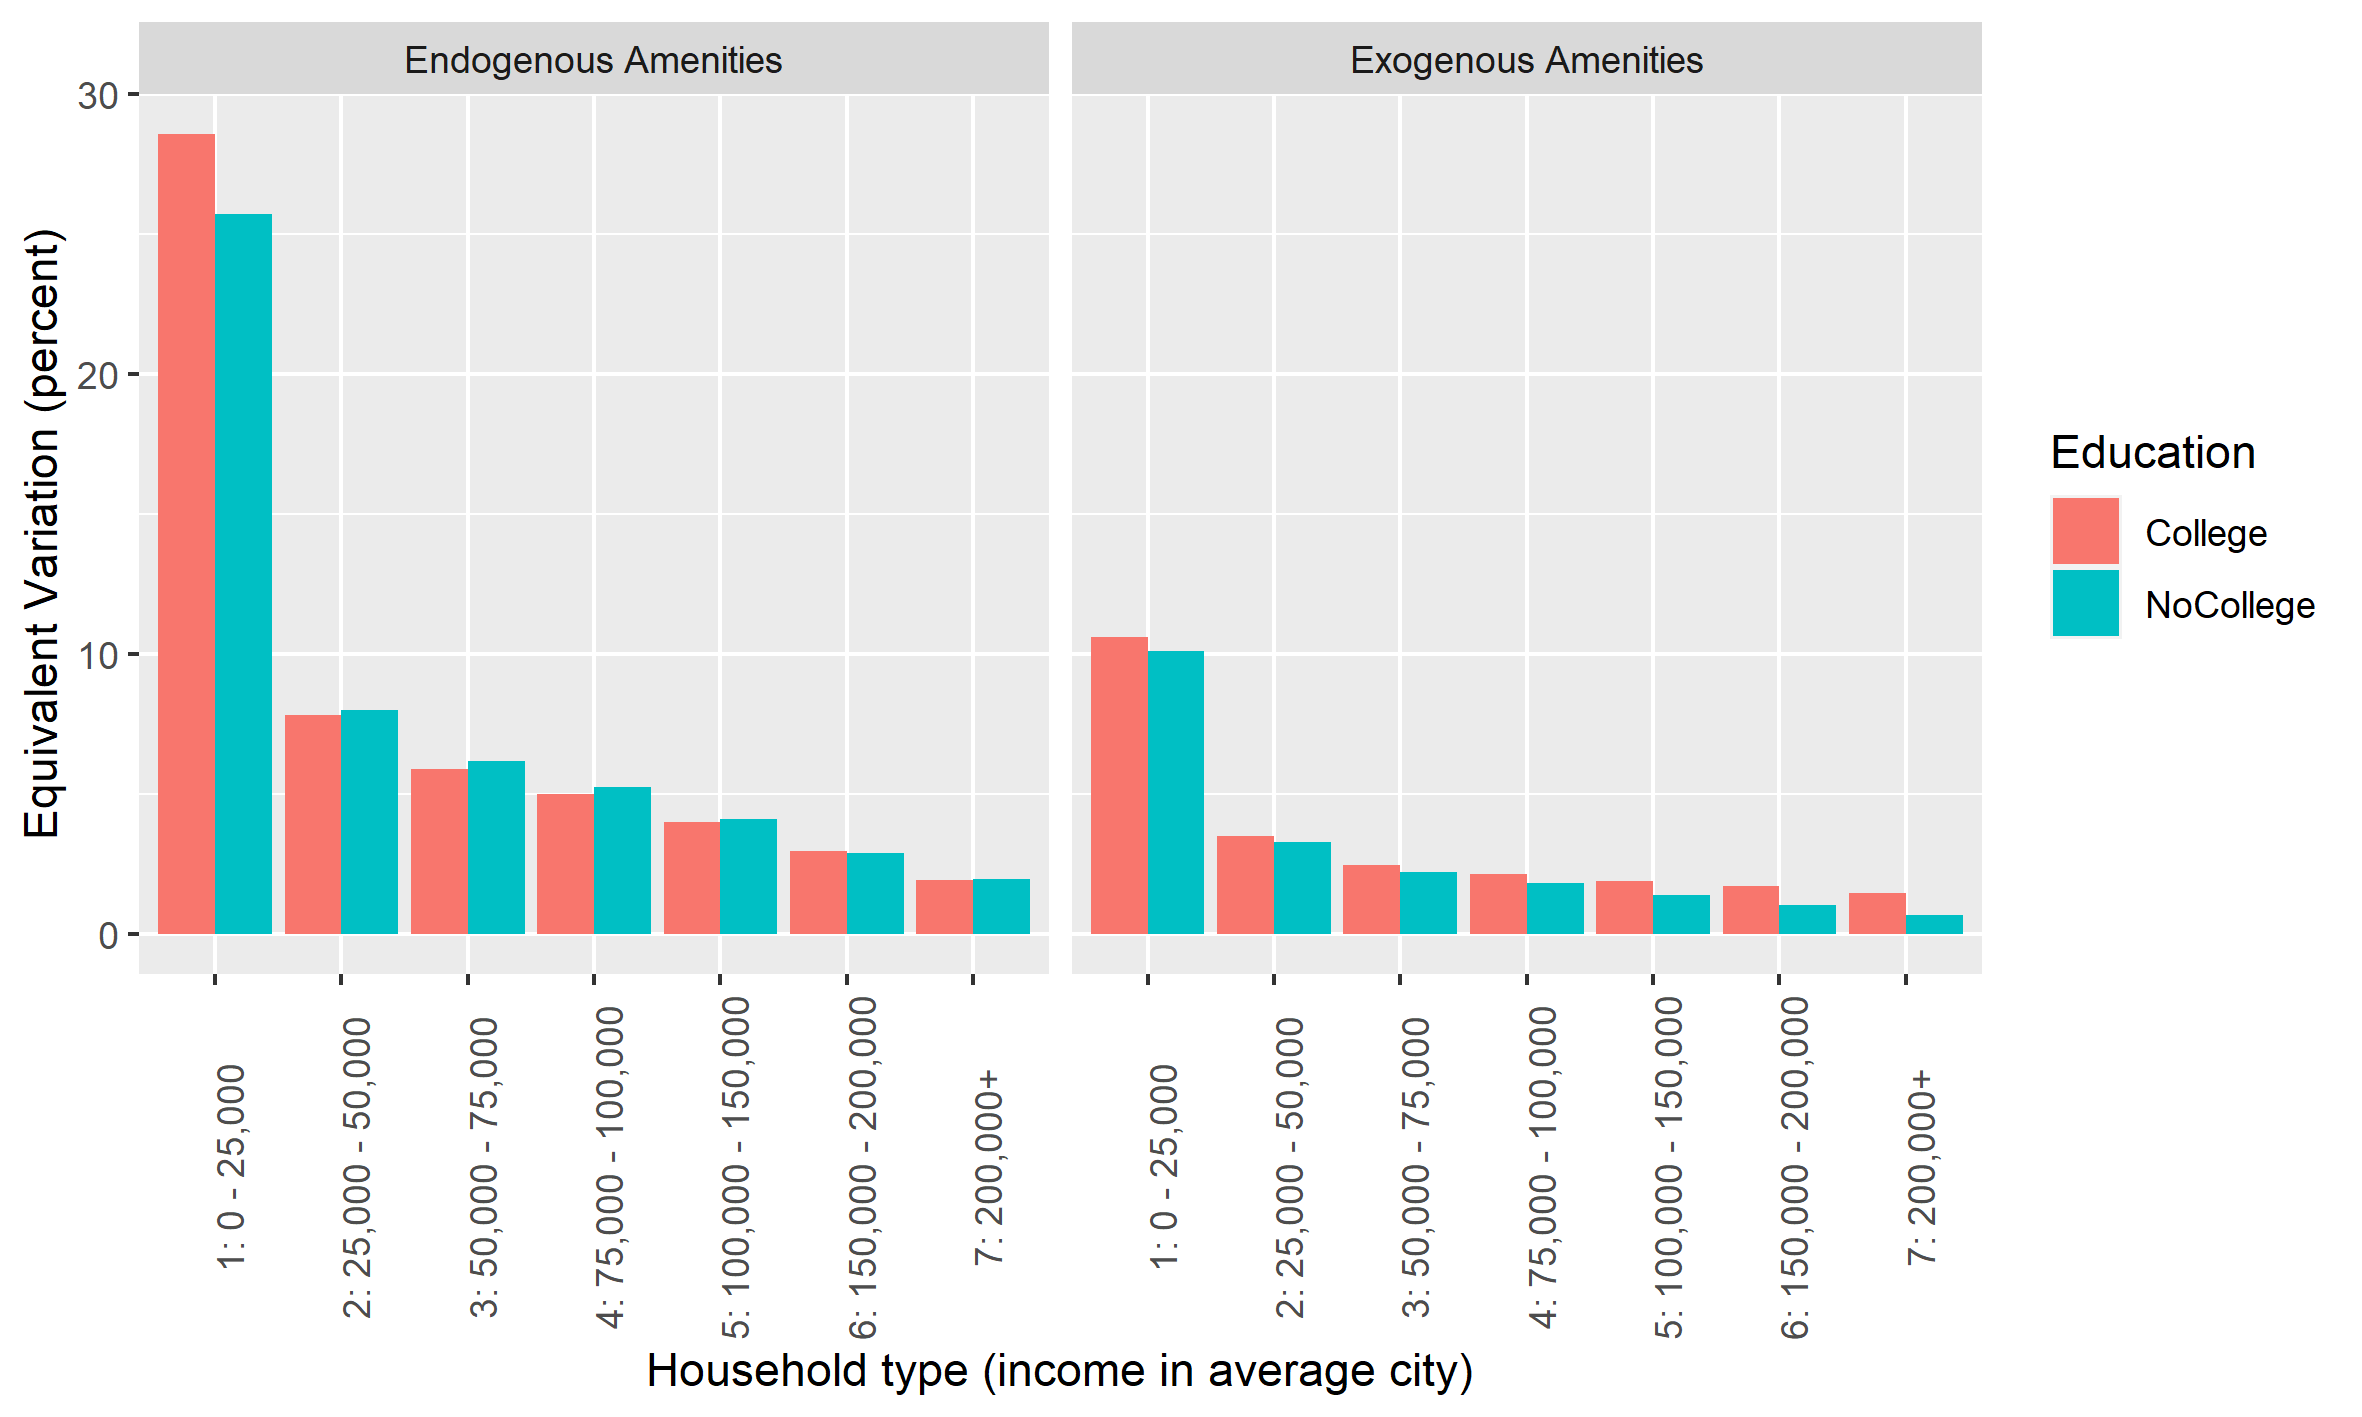
\includegraphics[width=1.1\textwidth]{Welfare.png}
		\caption{Equivalent variation by household type}\label{welfare_ctfl}
	\end{center}
\end{figure}

\paragraph*{}
How can we rationalize the fact that all workers gain, and that these gains are bolstered by endogenous changes in amenities? One potential explanation is through the labour productivity channel -- there are more people in more productive cities. However, I show that this cannot be the case; aggregate labour productivity is essentially \textit{unchanged} in transition to the counterfactual equilibrium, in direct opposition to the literature \citep{hseihmoretti} \citep{durantonpugaurbgrowth} \citep{parkho} \citep{hop}\footnote{In particular, I find that aggregate labour productivity increases from $\$84,269$ to $\$84,310$ at the chosen parameter values. These differ substantially from the literature. For example, \cite{durantonpugaurbgrowth} find that eliminating housing supply restrictions (as defined in their model) would increase output per person by around $8.2\%$. \cite{hseihmoretti} estimate the number to be $3.2\%$ in an exercise where they increase the housing supply elasticity in San Jose, San Francisco and New York.}. In the context of the model, this finding can only be rationalized in two ways. On one hand, there may not be much movement across cities. On the other hand, this can be driven by the income sorting effect offsetting the influx of households into productive cities, considering lot sizes tend to be more stringent in them (see Fact \ref{Fact3}). To test both hypotheses, I plot the growth rate in the number of households against the growth rate in the average household income type $f$ across all cities in Figure \ref{city_inc_sorting}. The figure very clearly rules out that there isn't much movement of households toward productive cities, see Chicago, Houston, and San Jose. It instead shows that the income sorting mechanism is responsible for keeping the aggregate labor supply in each city practically unchanged.  

\begin{figure}[htbp]
\centering
		
		\makebox[\textwidth]{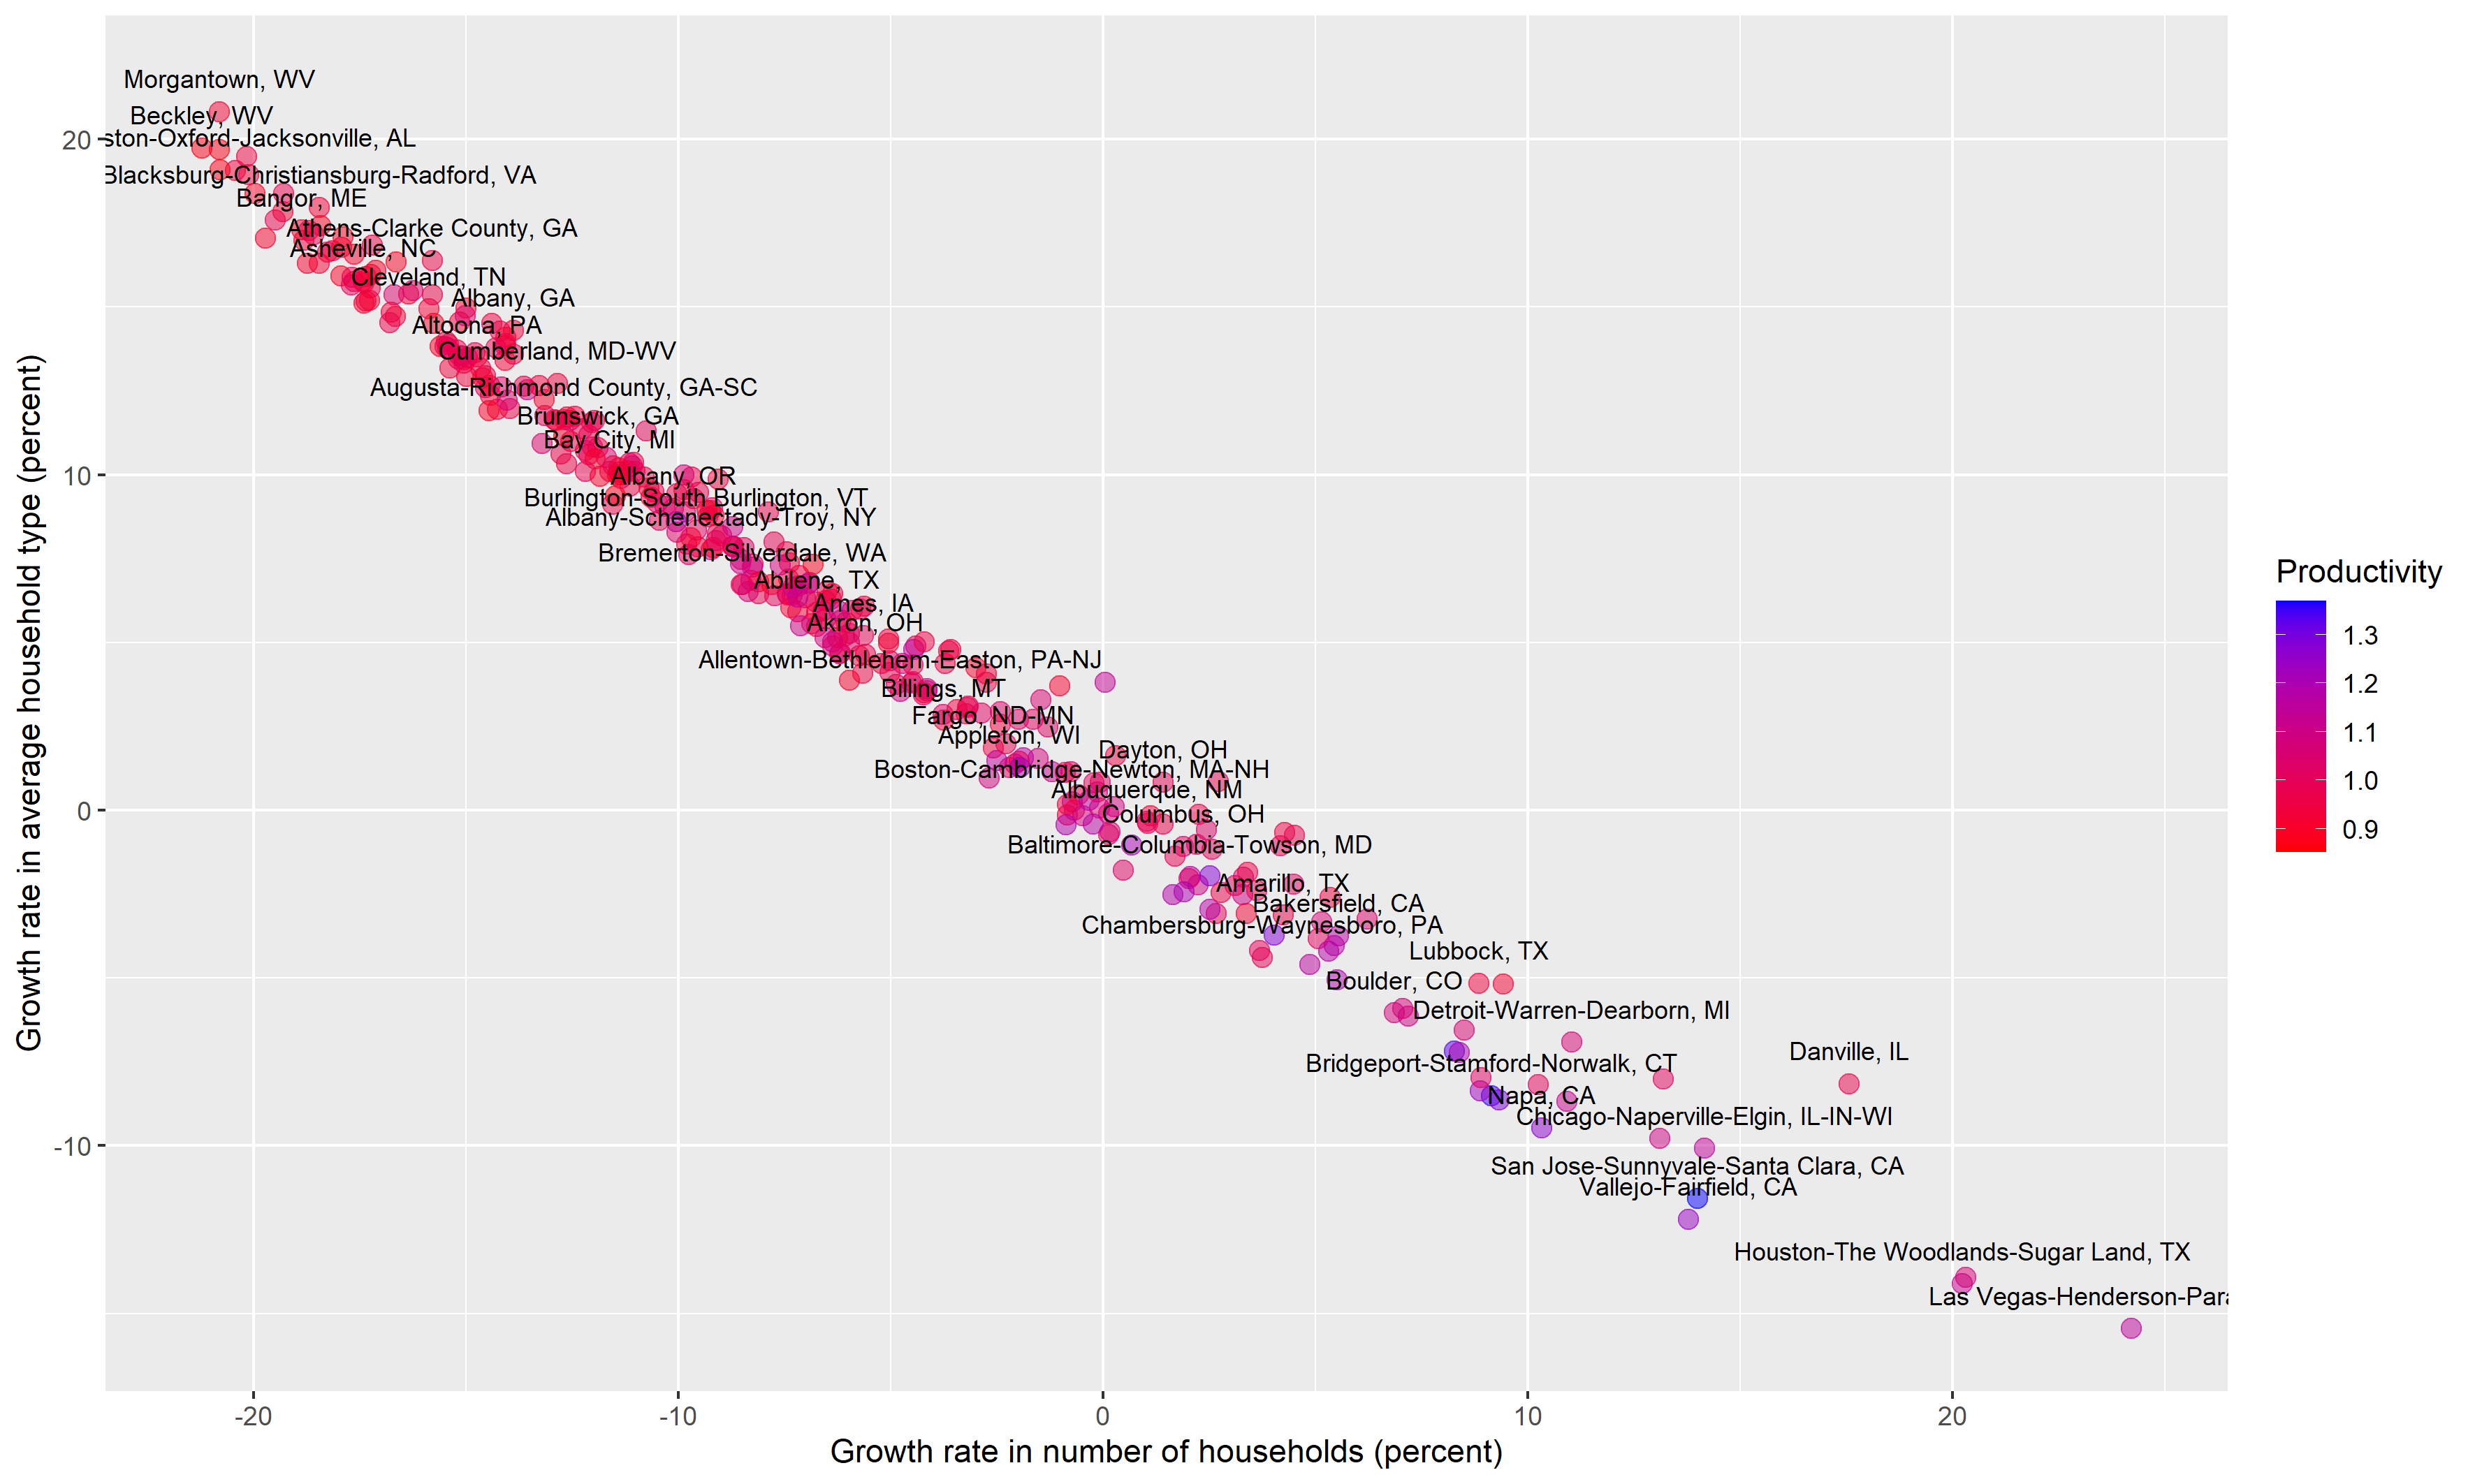
\includegraphics[width=1.4\textwidth]{IncomeSortingMovement.png}}
		\caption{City Income Sorting. The y axis is defined as the change in the average income that a household could earn in an average city. Productivity is defined as the average of the college and non-college wages per unit of labor. Correlation between growth rate in the number of households and productivity is approximately 0.55.}\label{city_inc_sorting}

\end{figure}

\paragraph*{}
The results in Figure \ref{welfare_ctfl} are instead driven by subtler forces. Eliminating minimum lot sizes causes large movements of very low income households (those that make less than $\$25,000$ in an average city) into previously regulated neighborhoods. As a result, the average amenities faced by this group actually \textit{decrease}\footnote{The average neighborhood income per household faced by low income households decreases from approximately $\$60,000$ to $\$35,000$.} because of their concentration in these neighborhoods, and the amenities faced by all other income groups increase. However, Figure \ref{welfare_ctfl} shows that these low income households benefit substantially from endogenous amenities, which appears to contradict this explanation. This can be reconciled by the fact that housing prices in these new concentrated low income neighborhoods decrease so strongly so as to lead to their net benefit\footnote{Housing prices faced by an average household from the lowest income group decreases from $\$1.76$ to $\$0.76$ per unit of housing services. All other groups see their prices increase at most by a factor of $1.2$.}. That is, these households benefit from the capitalization of these lower amenities into their housing prices. I want to stress that these results are driven by the current choice of the migration elasticity for this group, and they may change after the estimation procedure detailed in Section \ref{section:CalibrationIdent}. It could be that the observation of low income households in stringent neighborhoods leads to an overestimation of their type-specific amenities.

\paragraph*{Welfare of landlords} The welfare measurements in Figure \ref{welfare_ctfl} hint at the importance of changes in housing prices, and thus the rents earned on land by landlords. Consistent with the fact that housing prices faced by most income groups increase,  I find that the average (yearly) rent per acre over all neighborhoods rose from approximately $\$118,200$ to $\$124,200$. This increase in average rents is driven entirely by the endogenous amenities channel. This explains why the movement of land values differ in sign from \cite{parkho}, who does not model it. Moreover, considering average changes masks considerable heterogeneity across space. In fact, the growth in rents is reasonably biased toward locations that had high rents in the initial equilibrium. Using OLS, I find that on average land with initially $\$1$ higher rents are associated with approximately $\$1.8$ higher rents in the counterfactual. 

\paragraph*{}
Given that both landlords and workers generally benefit, why do these regulations persist? The obvious explanation is one consistent with the model: landlords in initially highly regulated neighborhoods lose after the reform, and thus have the political incentive to lobby against it. Using OLS and conditioning on neighborhoods that had a minimum lot size, I find that a one standard deviation increase in the yearly rent associated with a minimal lot (our measure of the stringency of lot size regulation) in the initial equilibrium is associated with approximately $30\%$ lower rents per acre after the reform. Moreover, initial stringency explains over $50\%$ of the variation in this regression. This represents a substantial deterioration of the amenity value of these neighborhoods\footnote{In reality, the relationship between initial stringency and differences in prices after reform are highly nonlinear. They cannot be extrapolated to extremely regulated neighborhoods, whom tend to have positive errors in the regression.}, and corroborates the plausibly causal estimates of  \cite{Song}, \cite{kulka} and \cite{KSC}. 

\paragraph*{Sorting within cities}  I have claimed that the differences in density gradients and income sorting patterns across cities are driven in part by lot size restrictions, and that these matter for welfare. The counterfactual exercise in this section supports both claims. Since the model matches the population and income distributions used to construct these facts very closely\footnote{There are some numerically small differences between the data used to construct the facts and the data used in the model. These arise from differences in sample (I drop approximately 6000 of the 177,000 block groups in which hedonic prices, income distributions and regulation could not be constructed, and I use an aggregated local income distributions to construct averages). These differences do not change the facts at all.}, I repeat the analysis in Figures \ref{Blockdens_dist} and \ref{incomesorting} using counterfactual equilibrium outcomes, and report the results in Figures \ref{ctfl_density_dist} and \ref{ctfl_inc_sorting}, respectively.

\paragraph*{} 
The density gradients in Figure \ref{ctfl_density_dist} exhibit the same structure as those in the observation data used in Figure \ref{Blockdens_dist}. However, the differences in the density gradients have noticeably decreased. This can be directly measured by comparing the $l^{2}$ norm of the differences in the curves across samples, which falls over \textit{89 percent} in the counterfactual equilibrium. What we observe is a relatively large movement of workers from high density neighborhoods in expensive cities, given that these neighborhoods tend to have little or no lot size regulation (Fact \ref{Fact3}). Moreover, the types of households that comprise these movers tend to be of very low income. This is corroborated by the results in Figure \ref{ctfl_inc_sorting}, where  massive increases in average income occur exclusively in the high density neighborhoods of expensive cities. This inverts the negative relationship between density and income that we observe in the data. 

\begin{figure}[htbp]
	\centering
	
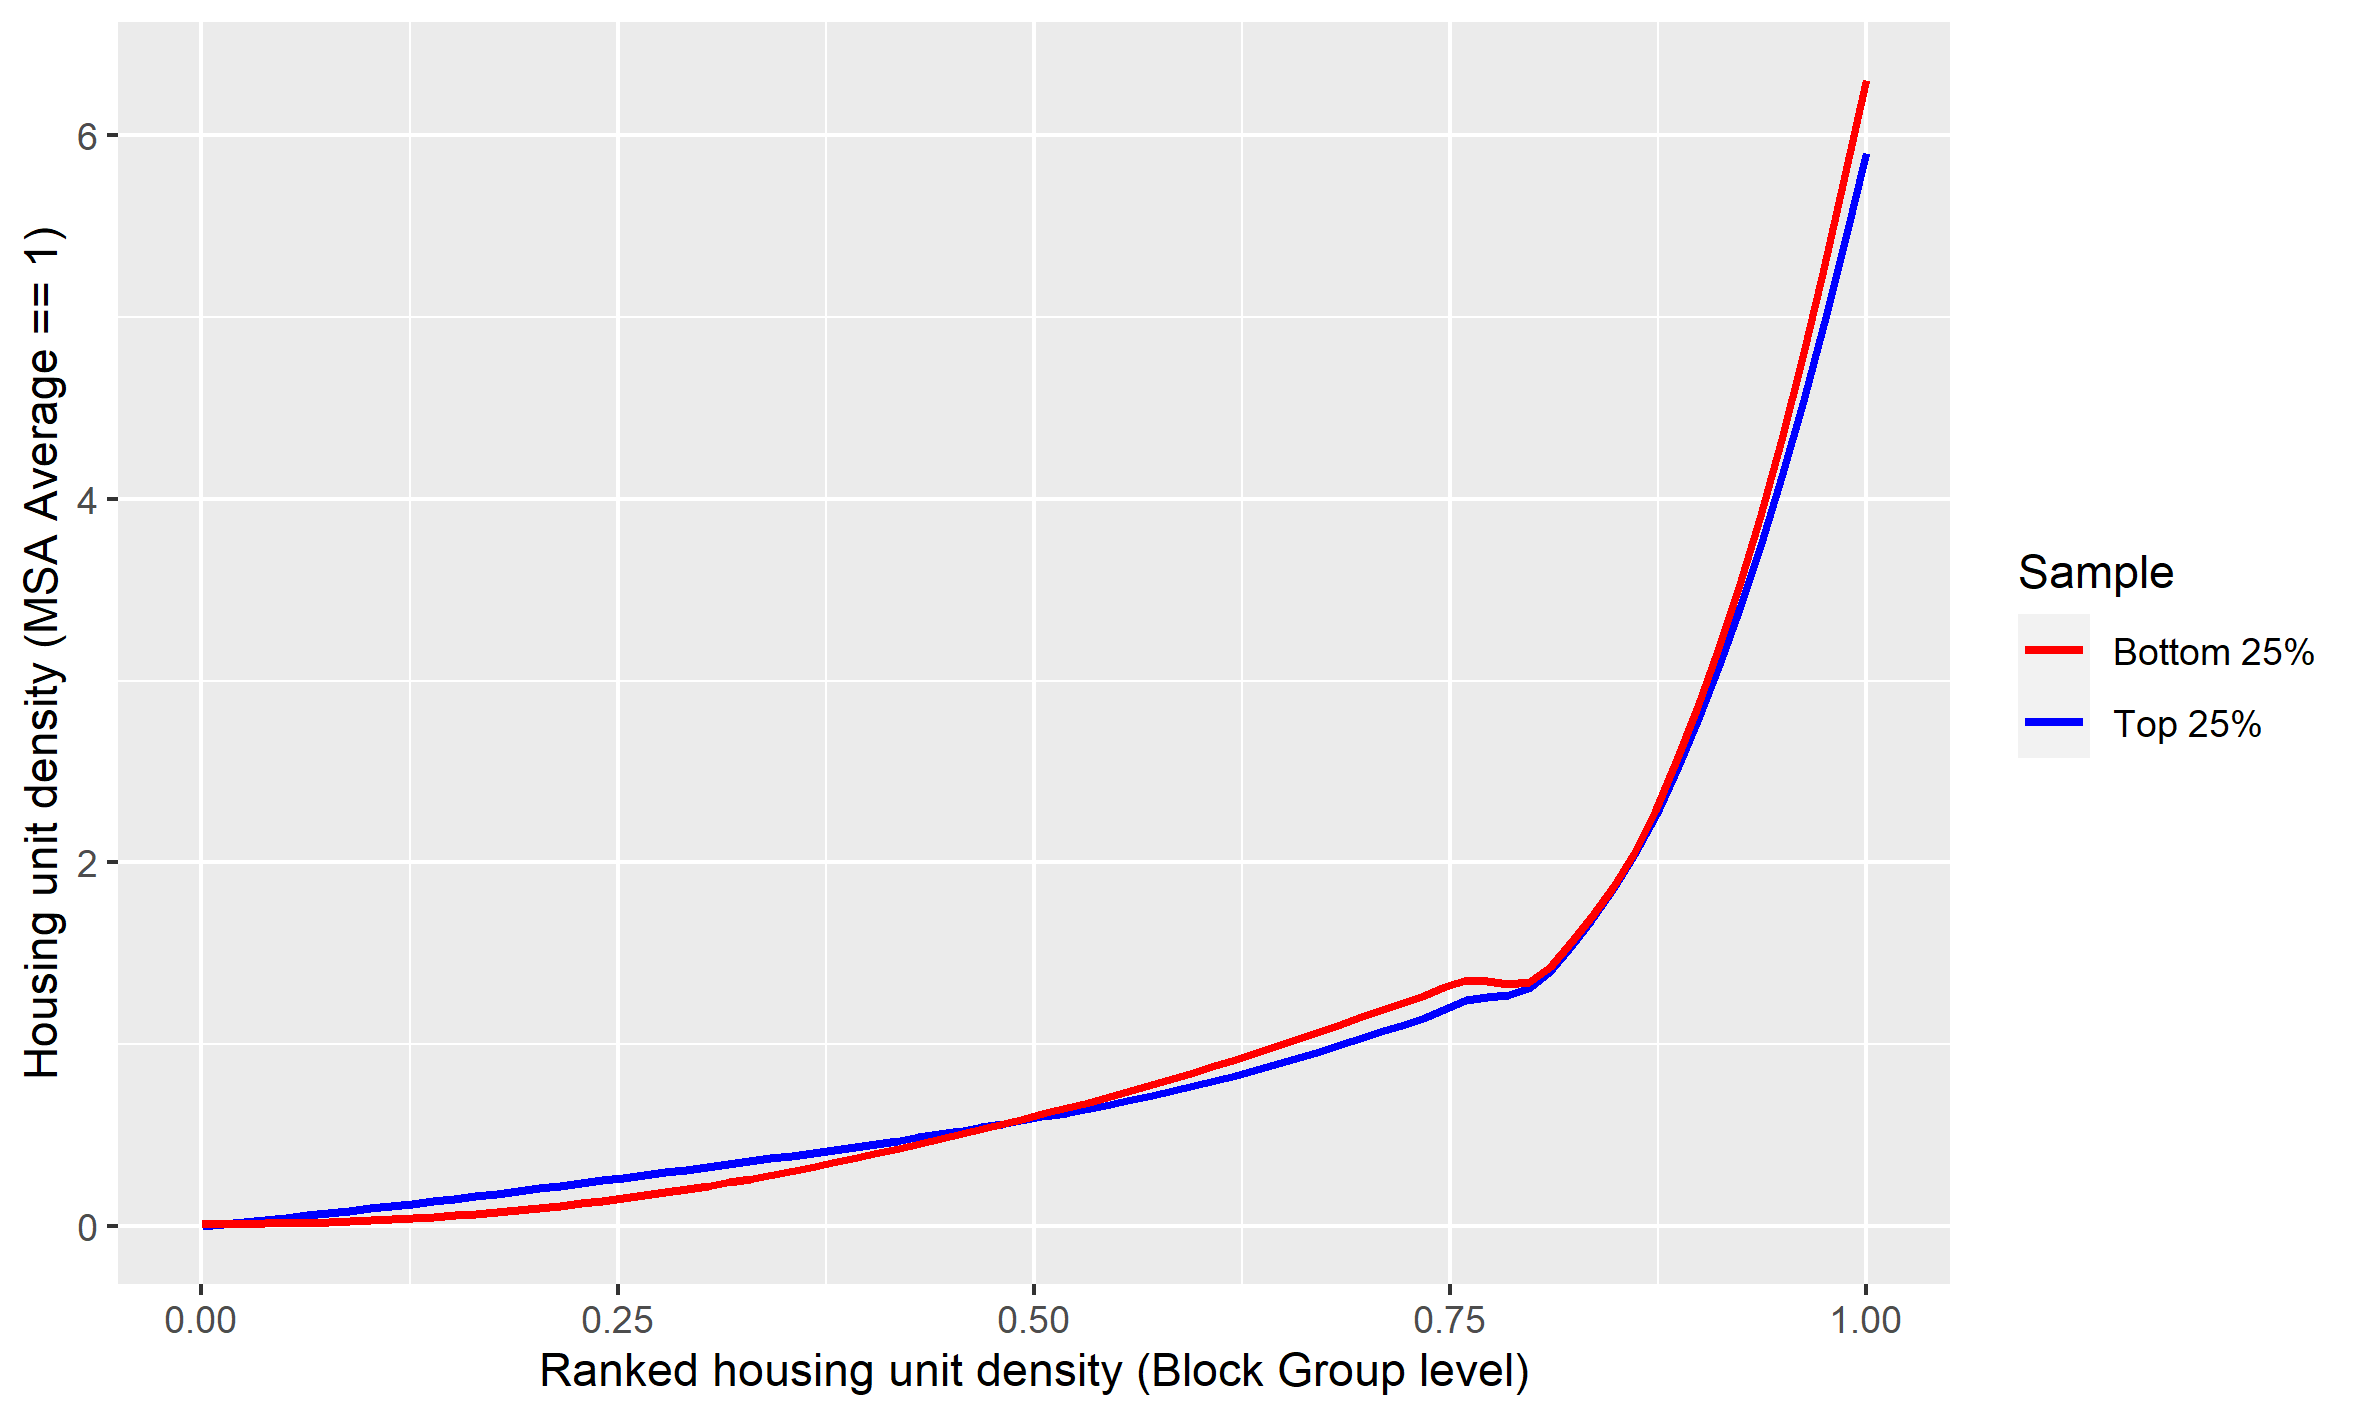
\includegraphics[width=\textwidth]{Density_dist_ctfcl.png}
	\caption{Density gradients in the counterfactual equilibrium. Loess regression with $\alpha = 0.5$. 95\% confidence intervals are reported. For the superstar sample, I take a random subset of the data to construct standard errors because of computational issues associated with Loess at large sample sizes.}\label{ctfl_density_dist}
	
\end{figure}

\begin{figure}[htbp]
	\centering
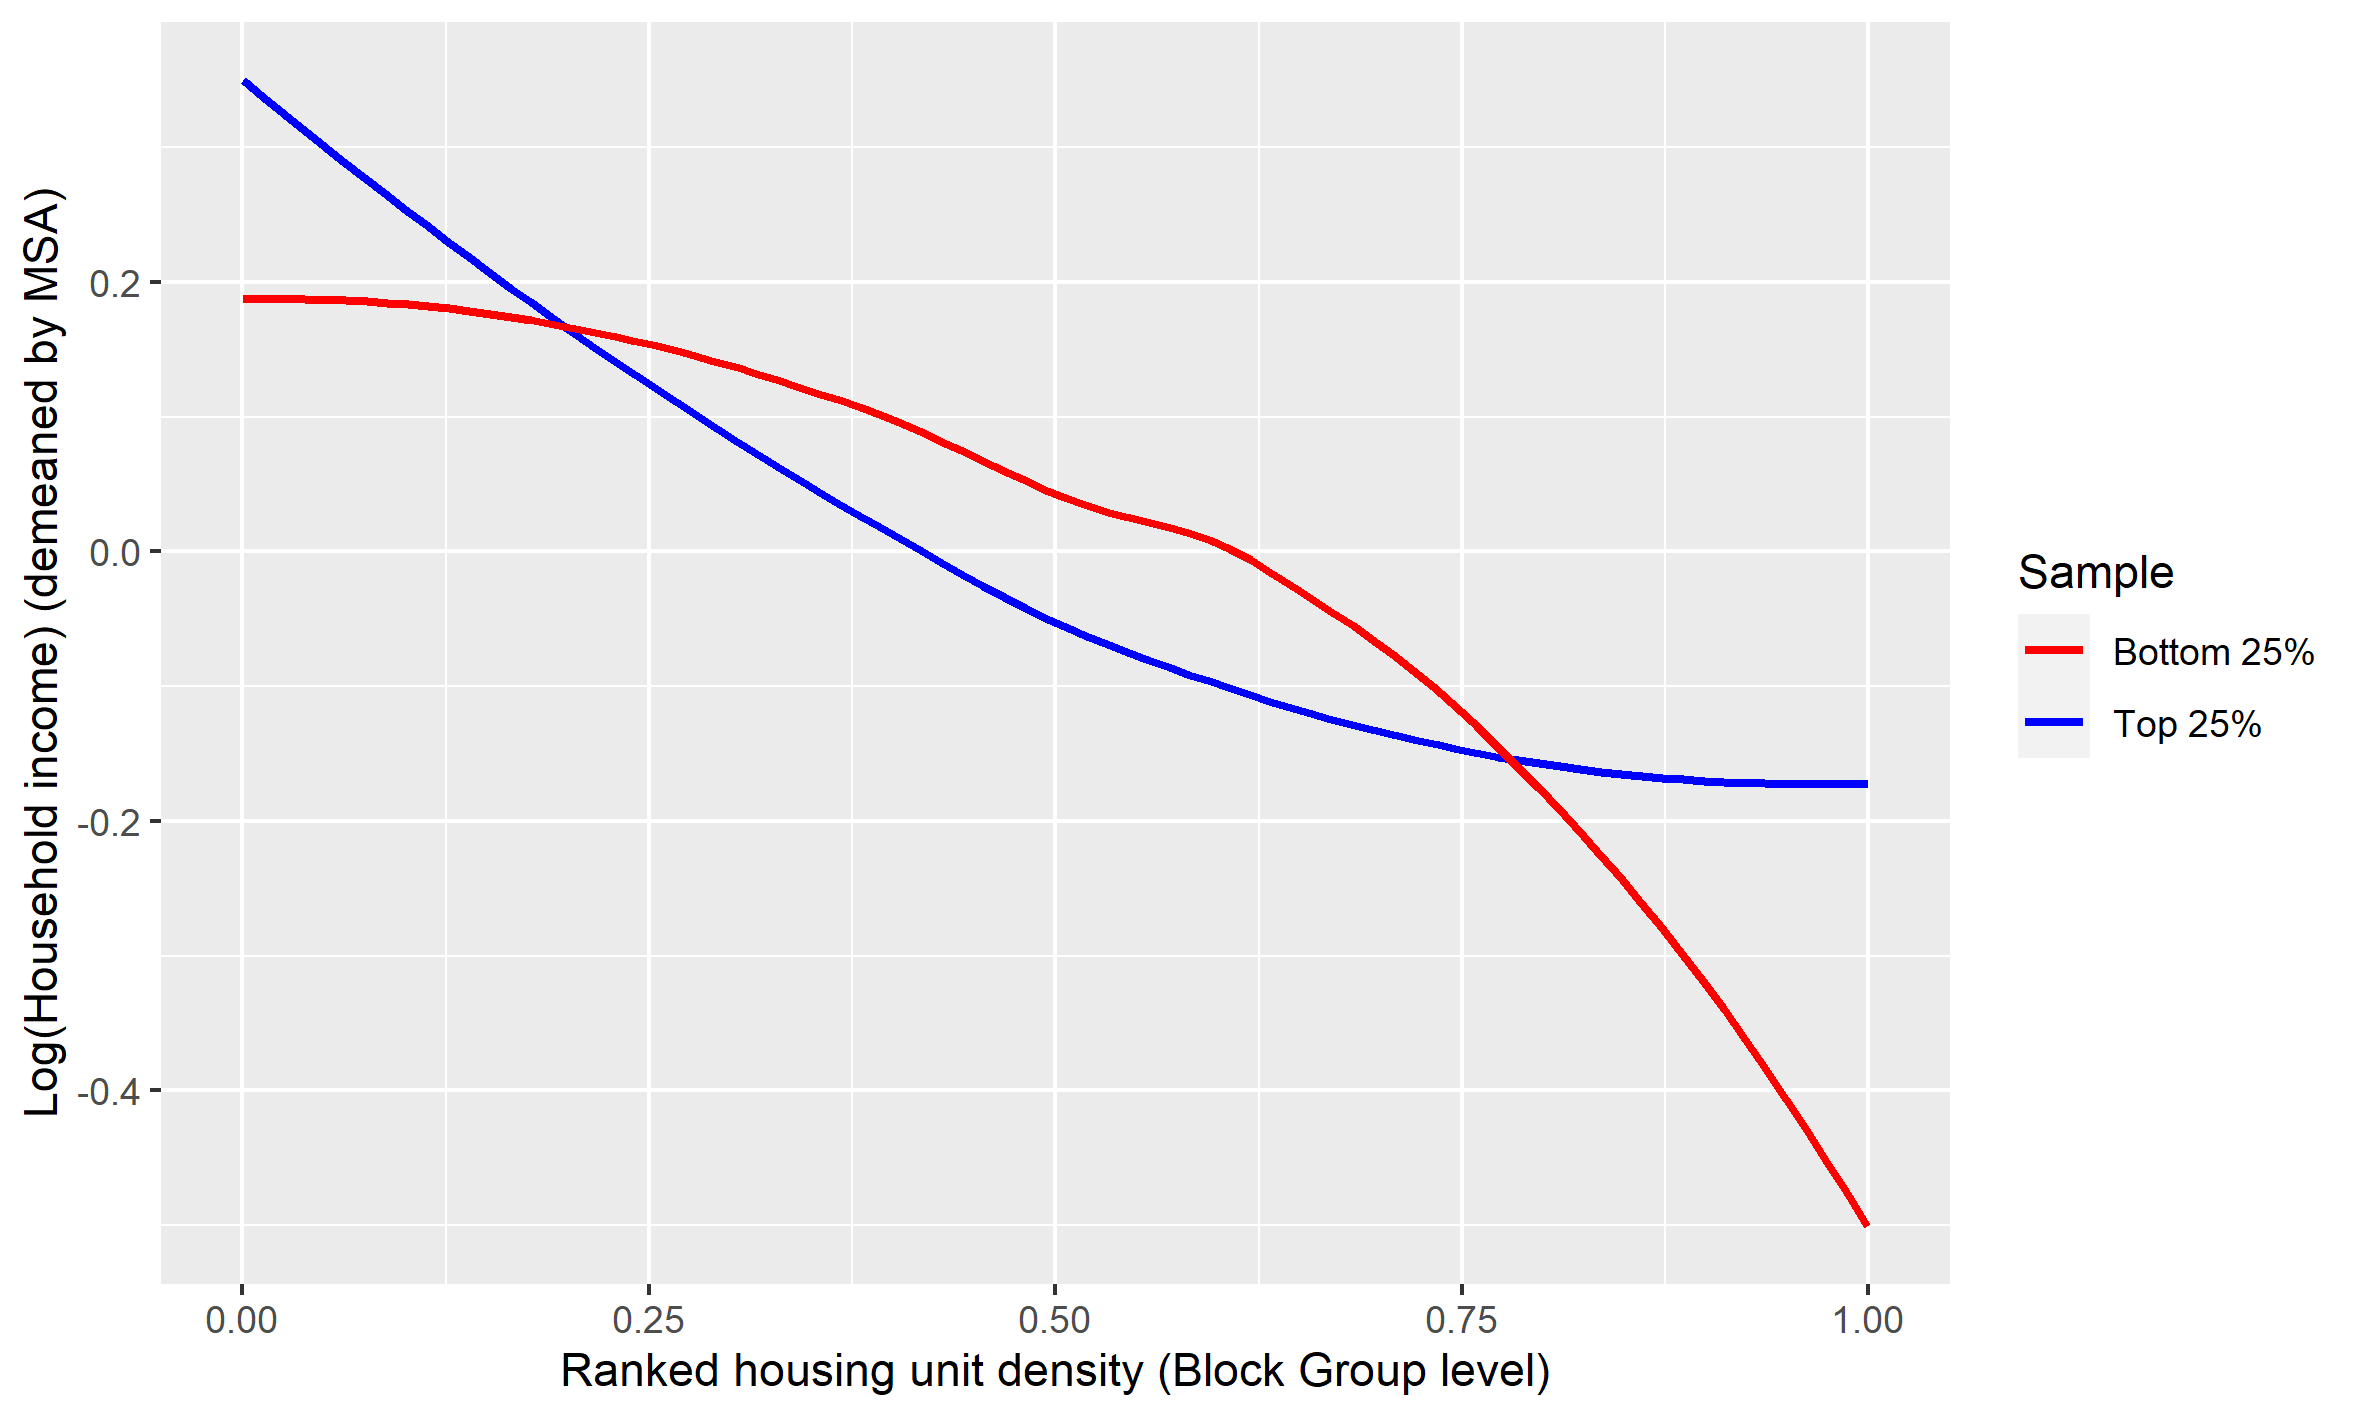
\includegraphics[width=\textwidth]{Income_dist_ctfcl.png}
	\caption{Income grandients in the counterfactual equilibrium. Loess regression with $\alpha = 1$. 95\% confidence intervals are reported. For the superstar sample, I take a random subset of the data to construct standard errors because of computational issues associated with Loess at large sample sizes.}\label{ctfl_inc_sorting}
	
\end{figure}




%%%%%%%%%%%%%%%%%%%%%%%%%%%%%%%%%%%%%%%%%%%%%%%%% %CONCLUSION%%%%%%%%%%%%%%%%%%%%%%%%%%%%%%%%%%%%%%%%%%%%%%%%%%%%%%%%%%%%%%%%%%%%%%%%%%%%%%%%%%%%%%%%%
%%%%%%%%%%%%%%%%%%%%%%%%%%%%%%%%%%%%%%%%%%%%%%%%%%


\section{Conclusion}
TBD

\newpage
\scriptsize
\bibliography{references.bib}

\newpage
\newpage
\appendix
\section{Appendix: Data and Facts Continued}\label{DataandFactsContinued}

\subsection{Figures}
\begin{figure}[hbpt]
\begin{center}
	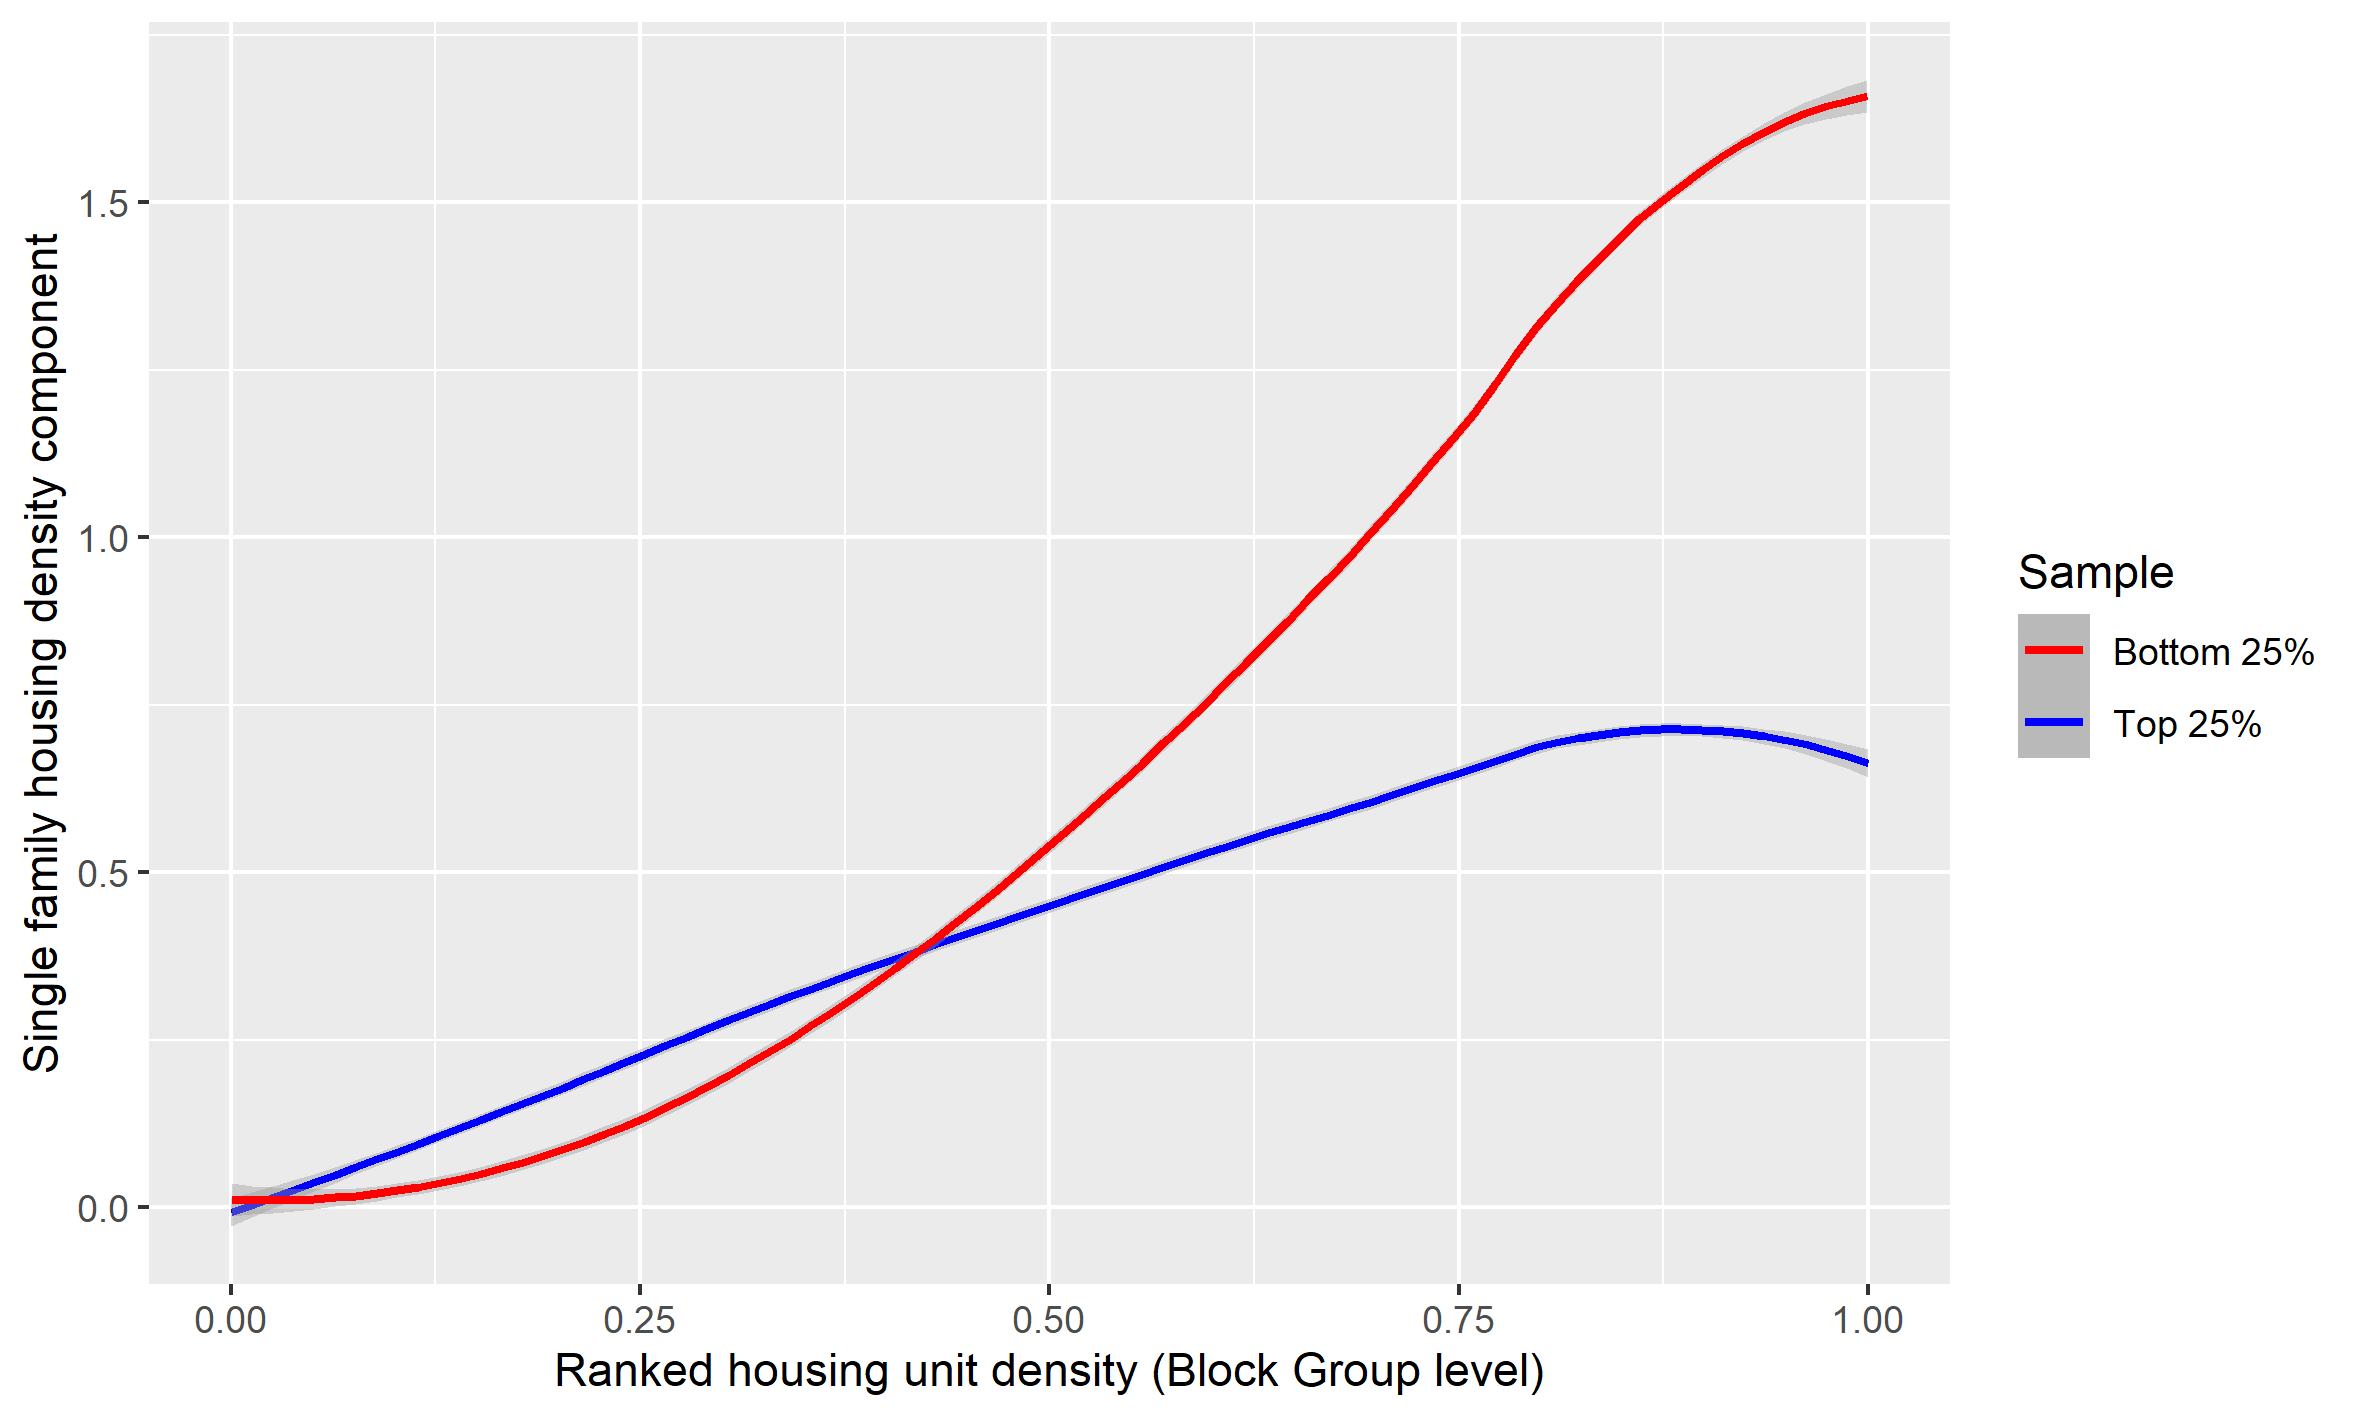
\includegraphics[width=0.9\textwidth]{singlefamily_dist.png}
	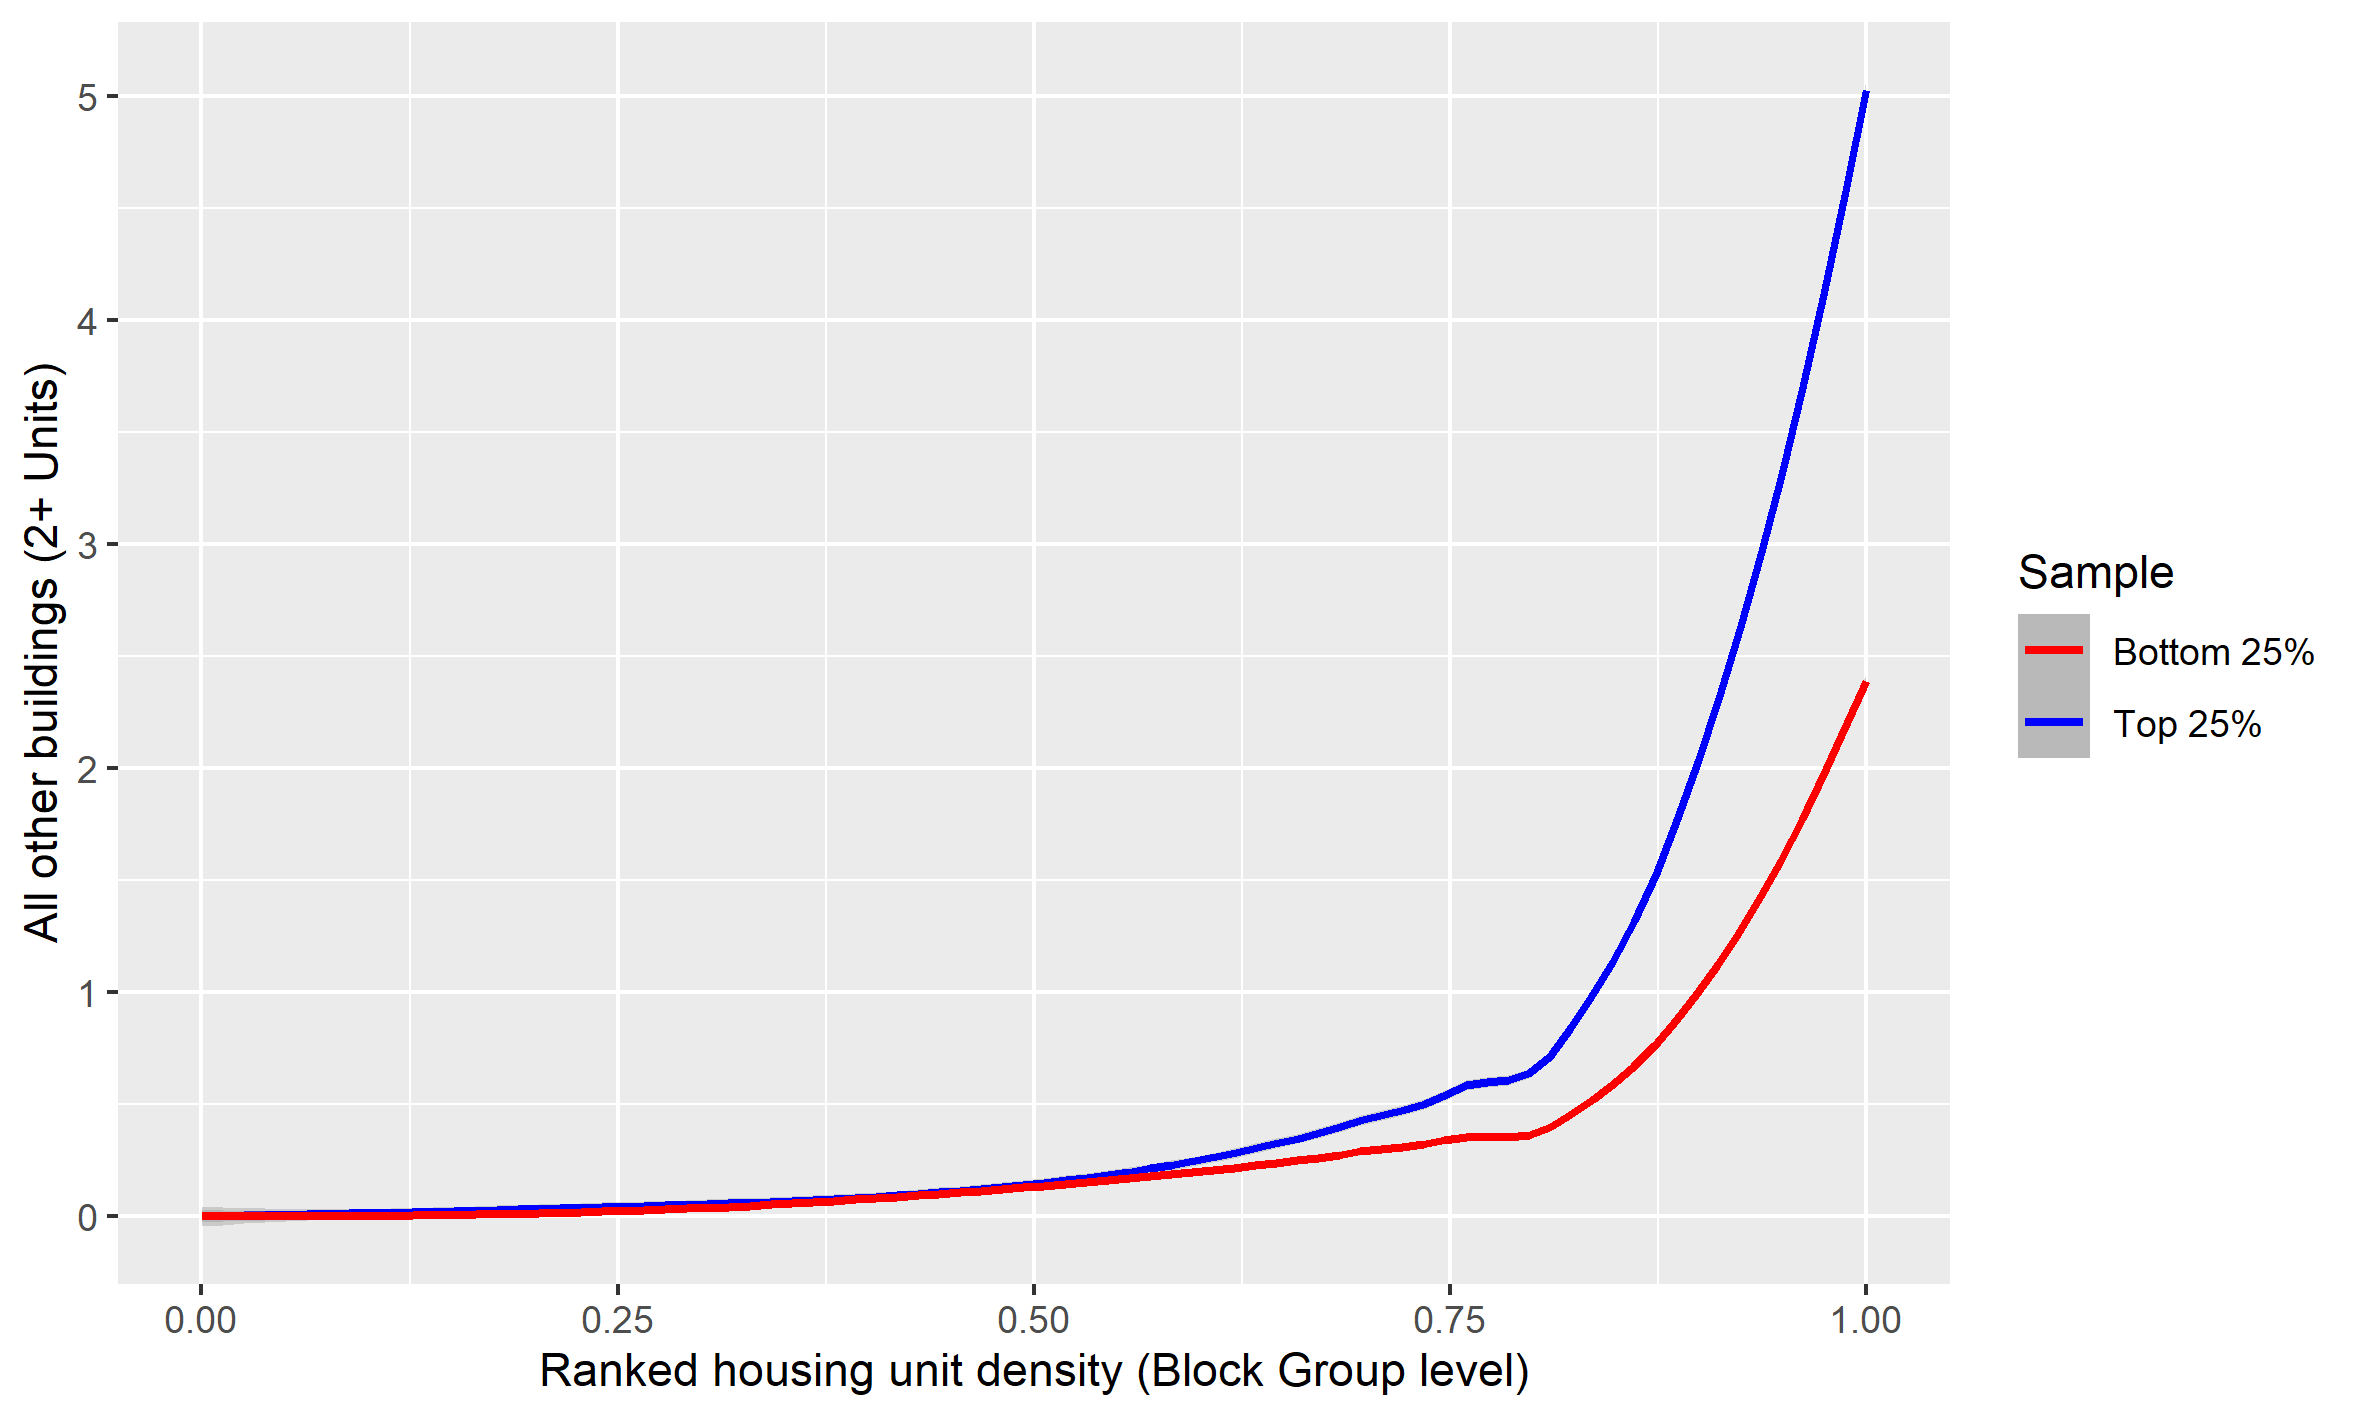
\includegraphics[width=0.9\textwidth]{2plusbuilding_dist.png}
	\caption{Loess regression with $\alpha = 0.5$. 95\% confidence intervals are reported. For the superstar sample, I take a random subset of the data to construct standard errors because of computational issues associated with Loess at large sample sizes.}\label{SingleFMargin}
\end{center}
\end{figure}

\begin{figure}[hbpt]
	\begin{center}
		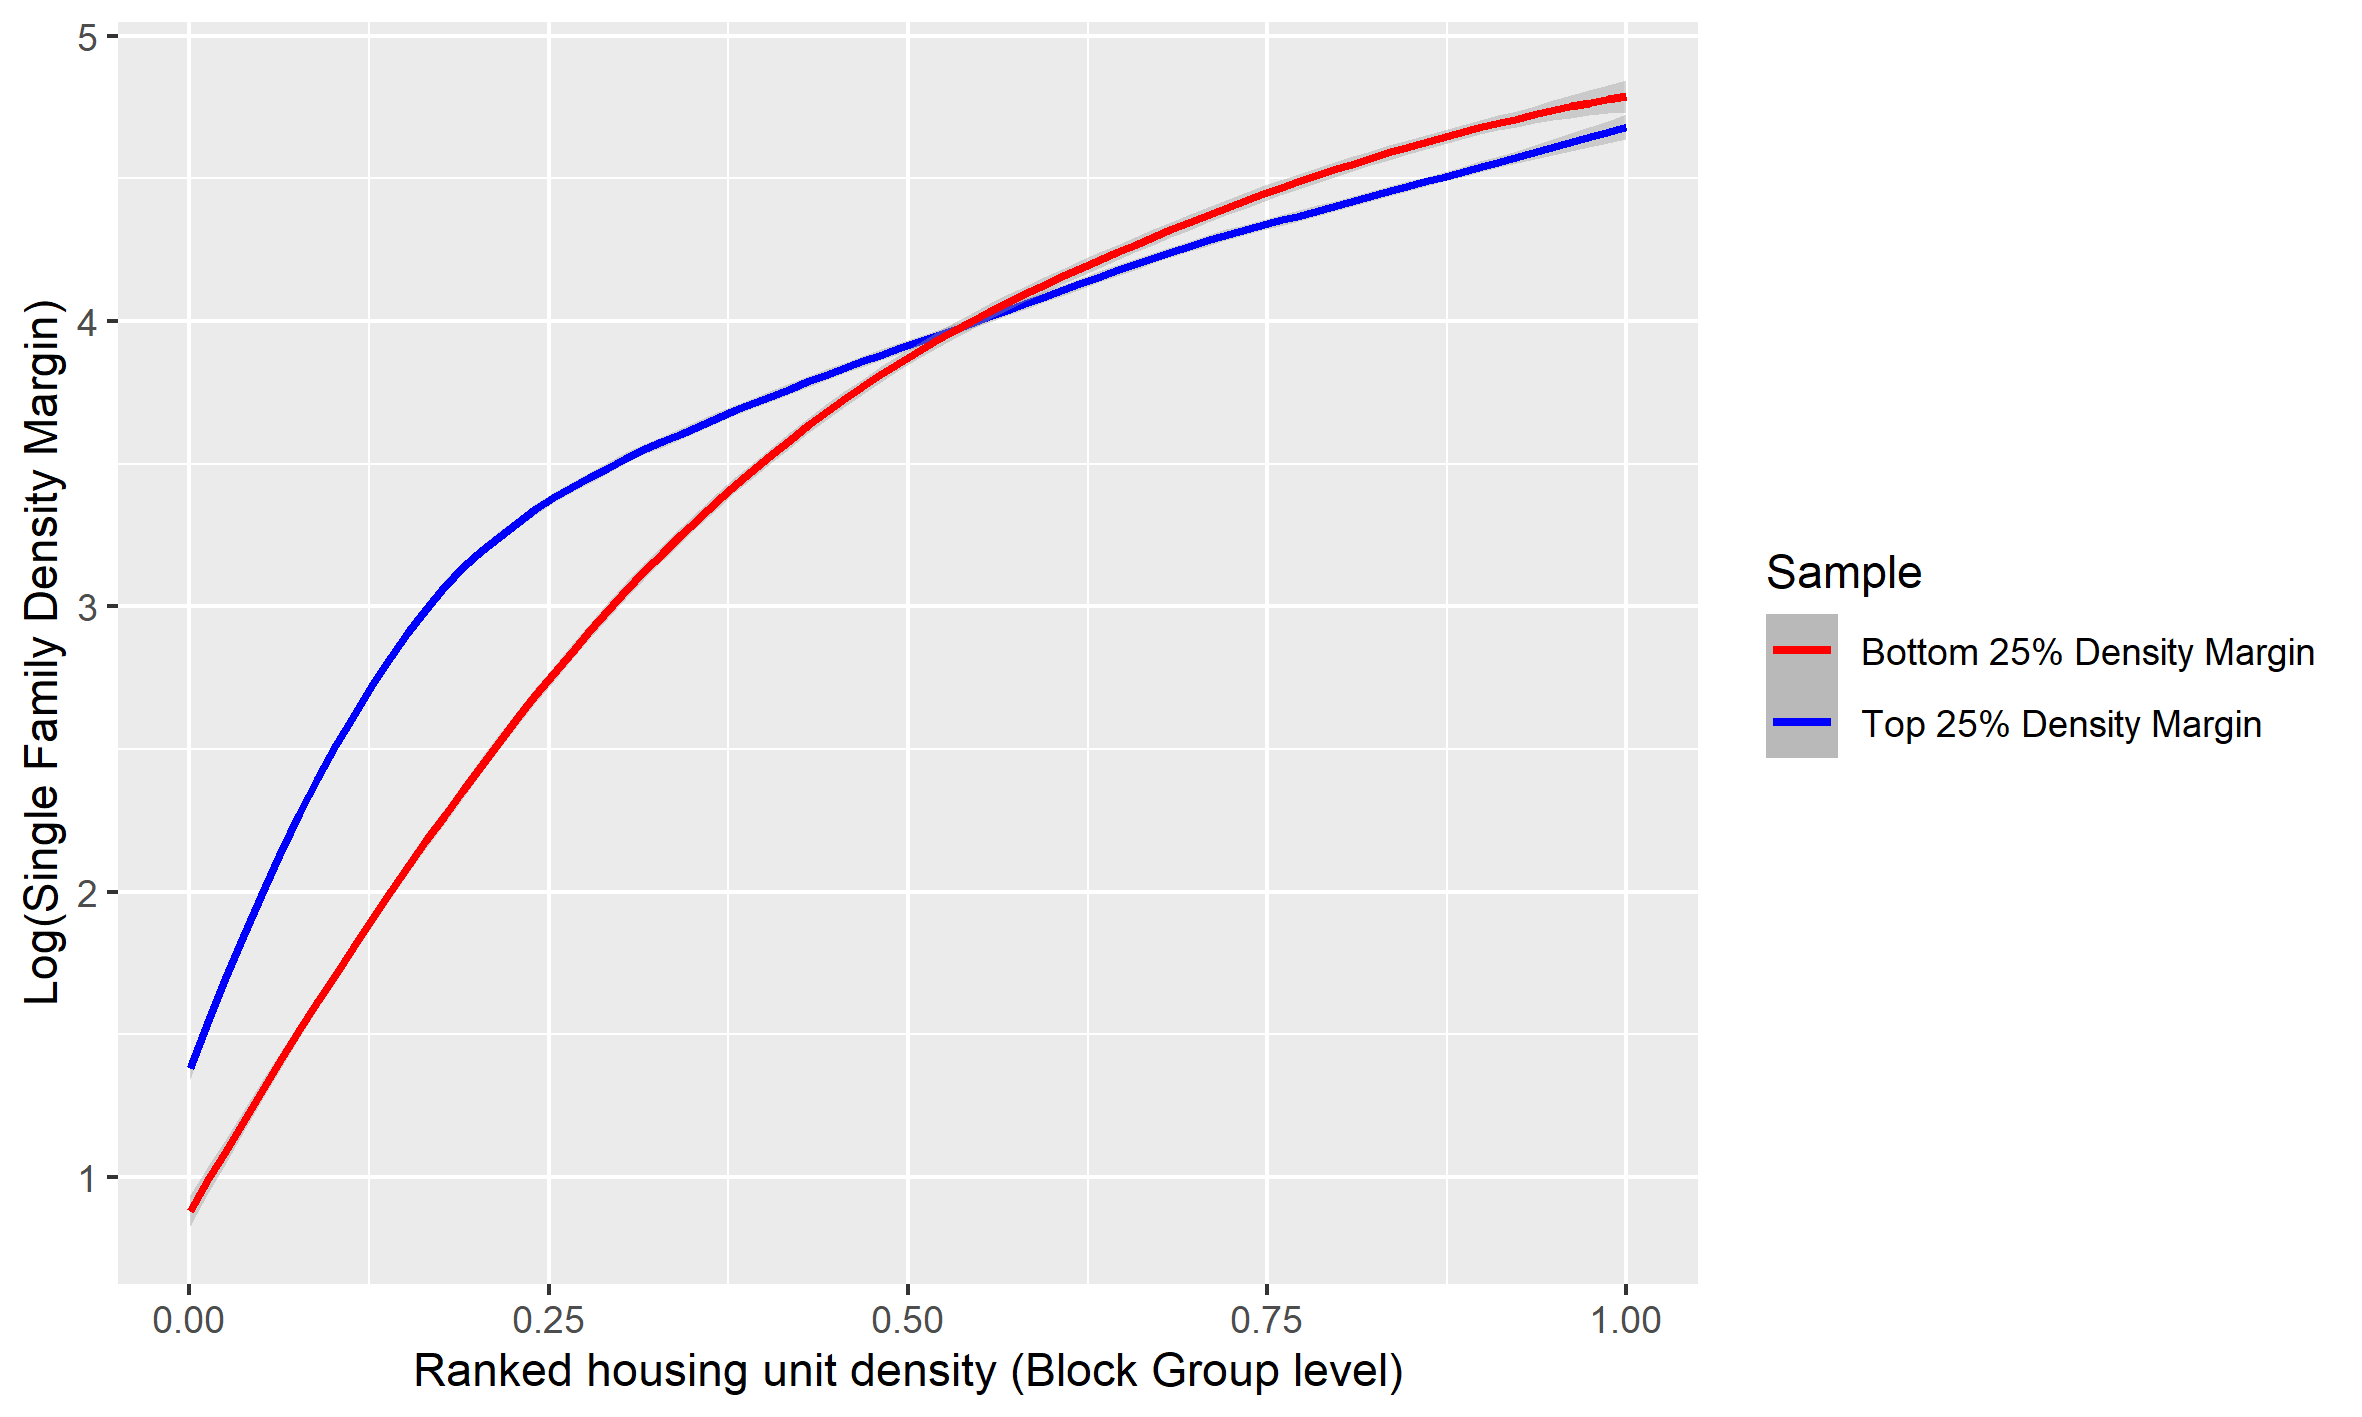
\includegraphics[width=\textwidth]{SingleFamilyDensity.png}
		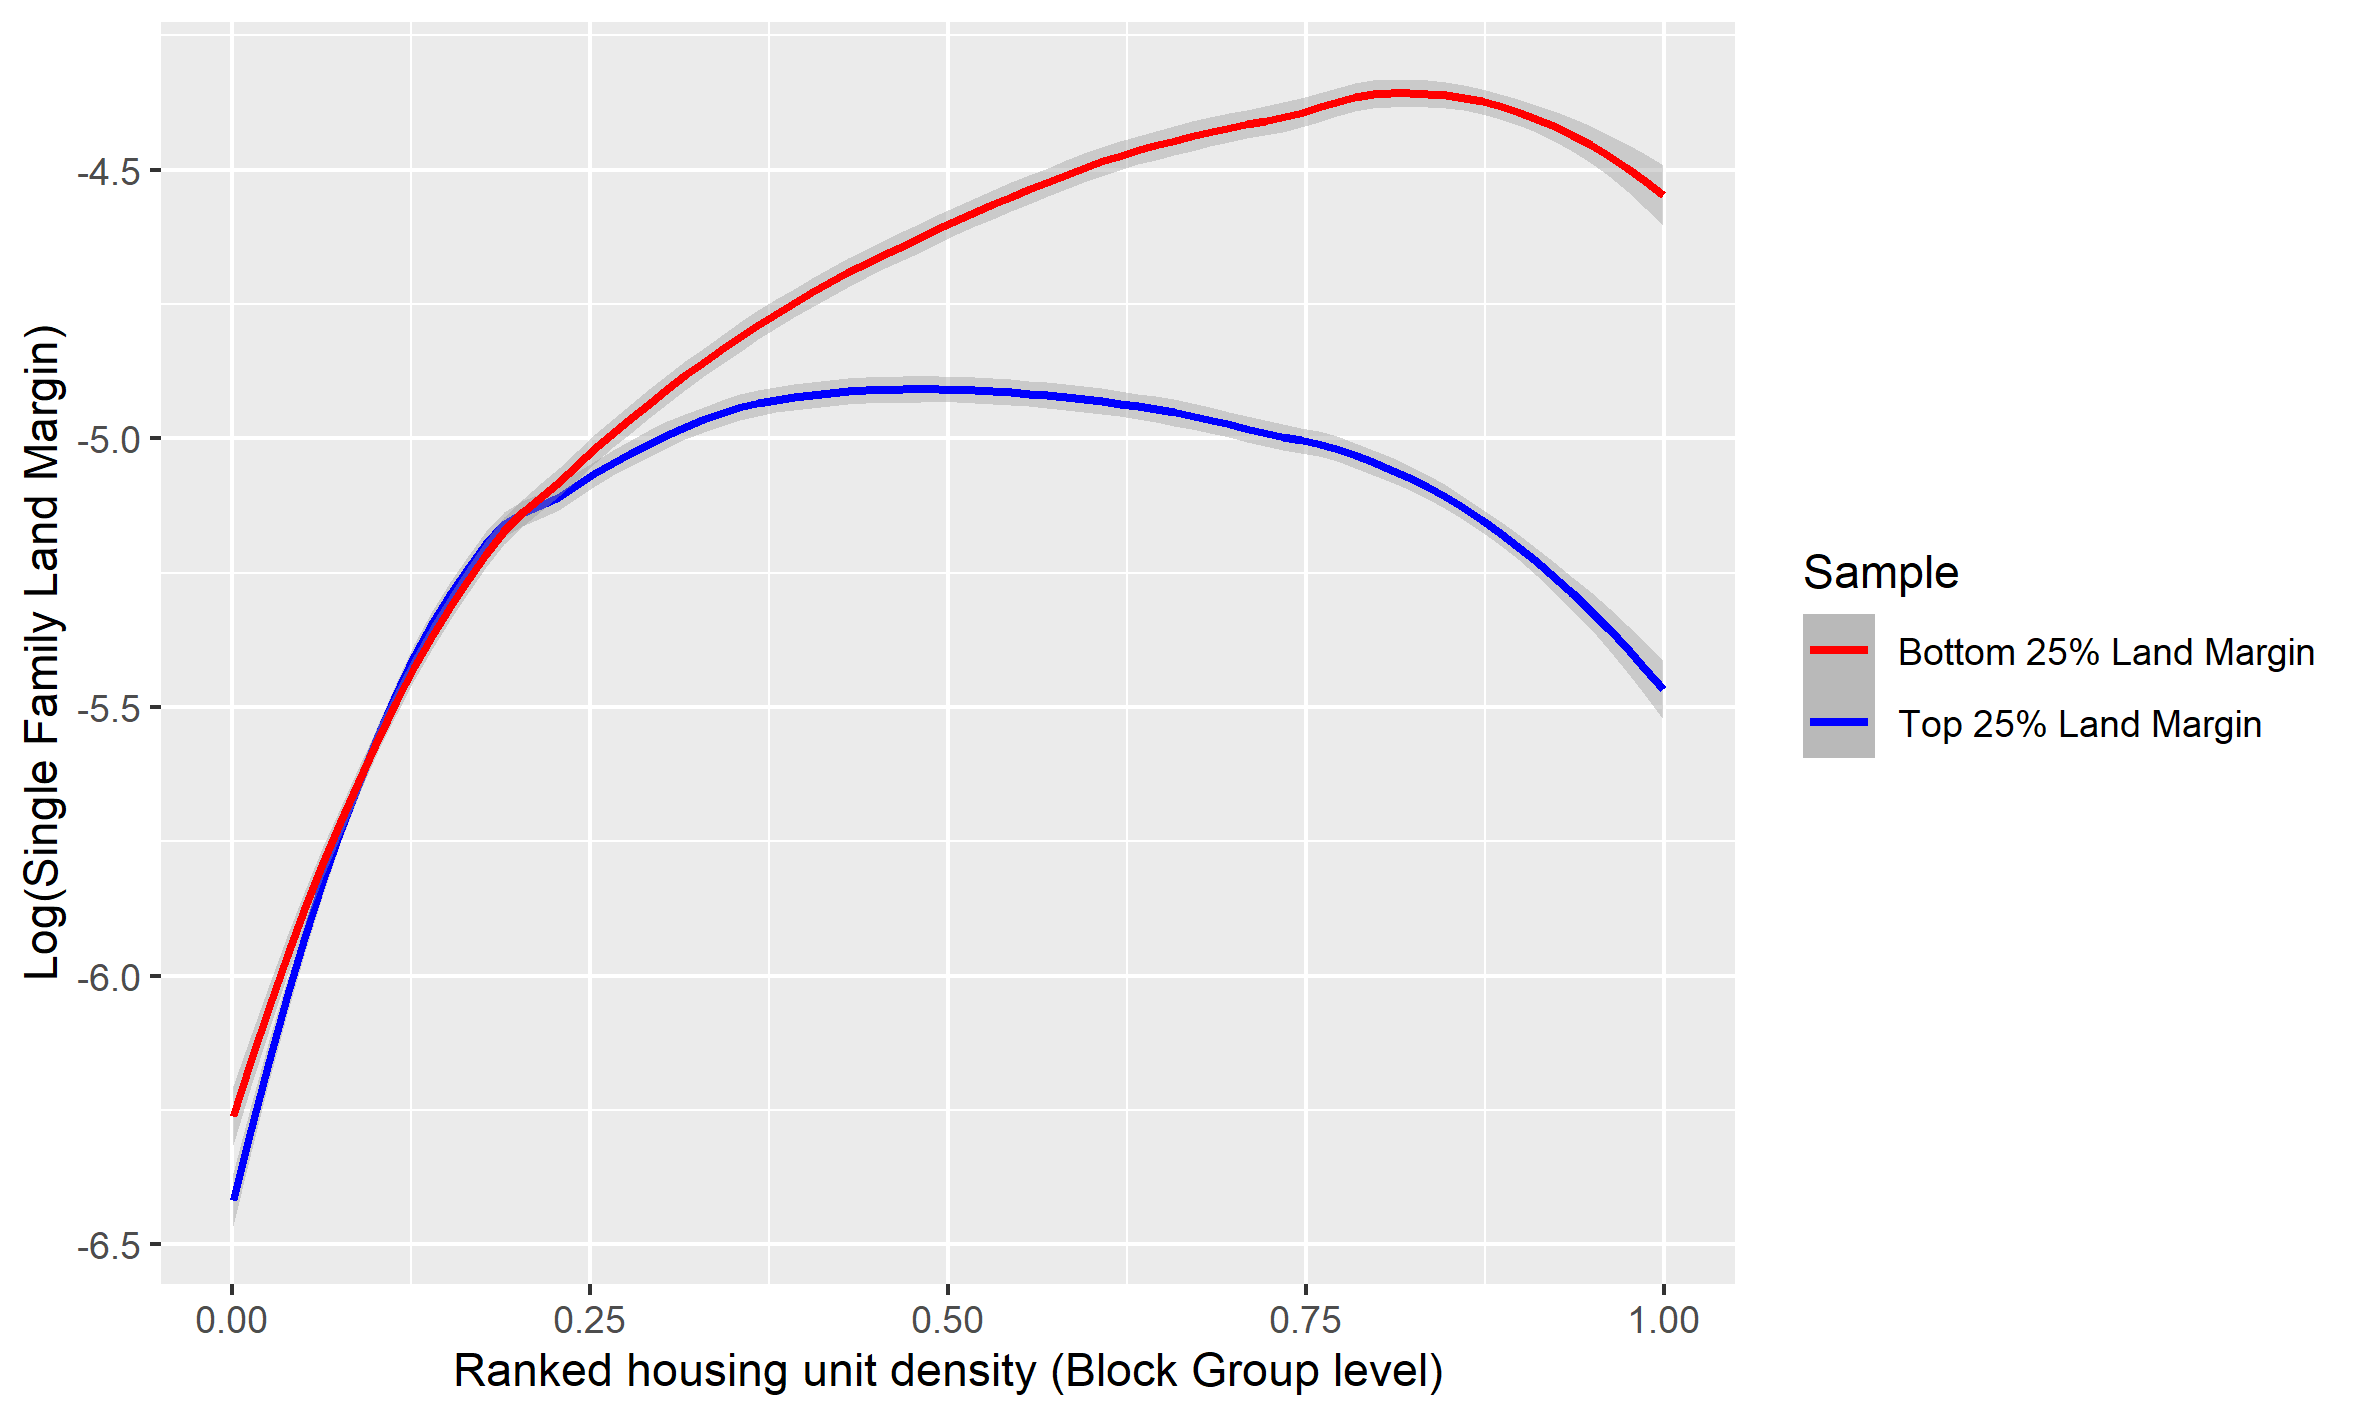
\includegraphics[width=\textwidth]{SingleFamilyLand.png}
		\caption{Loess regression with $\alpha = 0.5$. 95\% confidence intervals are reported. For the superstar sample, I take a random subset of the data to construct standard errors because of computational issues associated with Loess at large sample sizes.}\label{SingleFDensityMargin}
	\end{center}
\end{figure}

\newpage


\subsection{French Data Construction}\label{FrenchDFC}
Will be Completed
\begin{figure}[hbpt]
	\begin{center}
		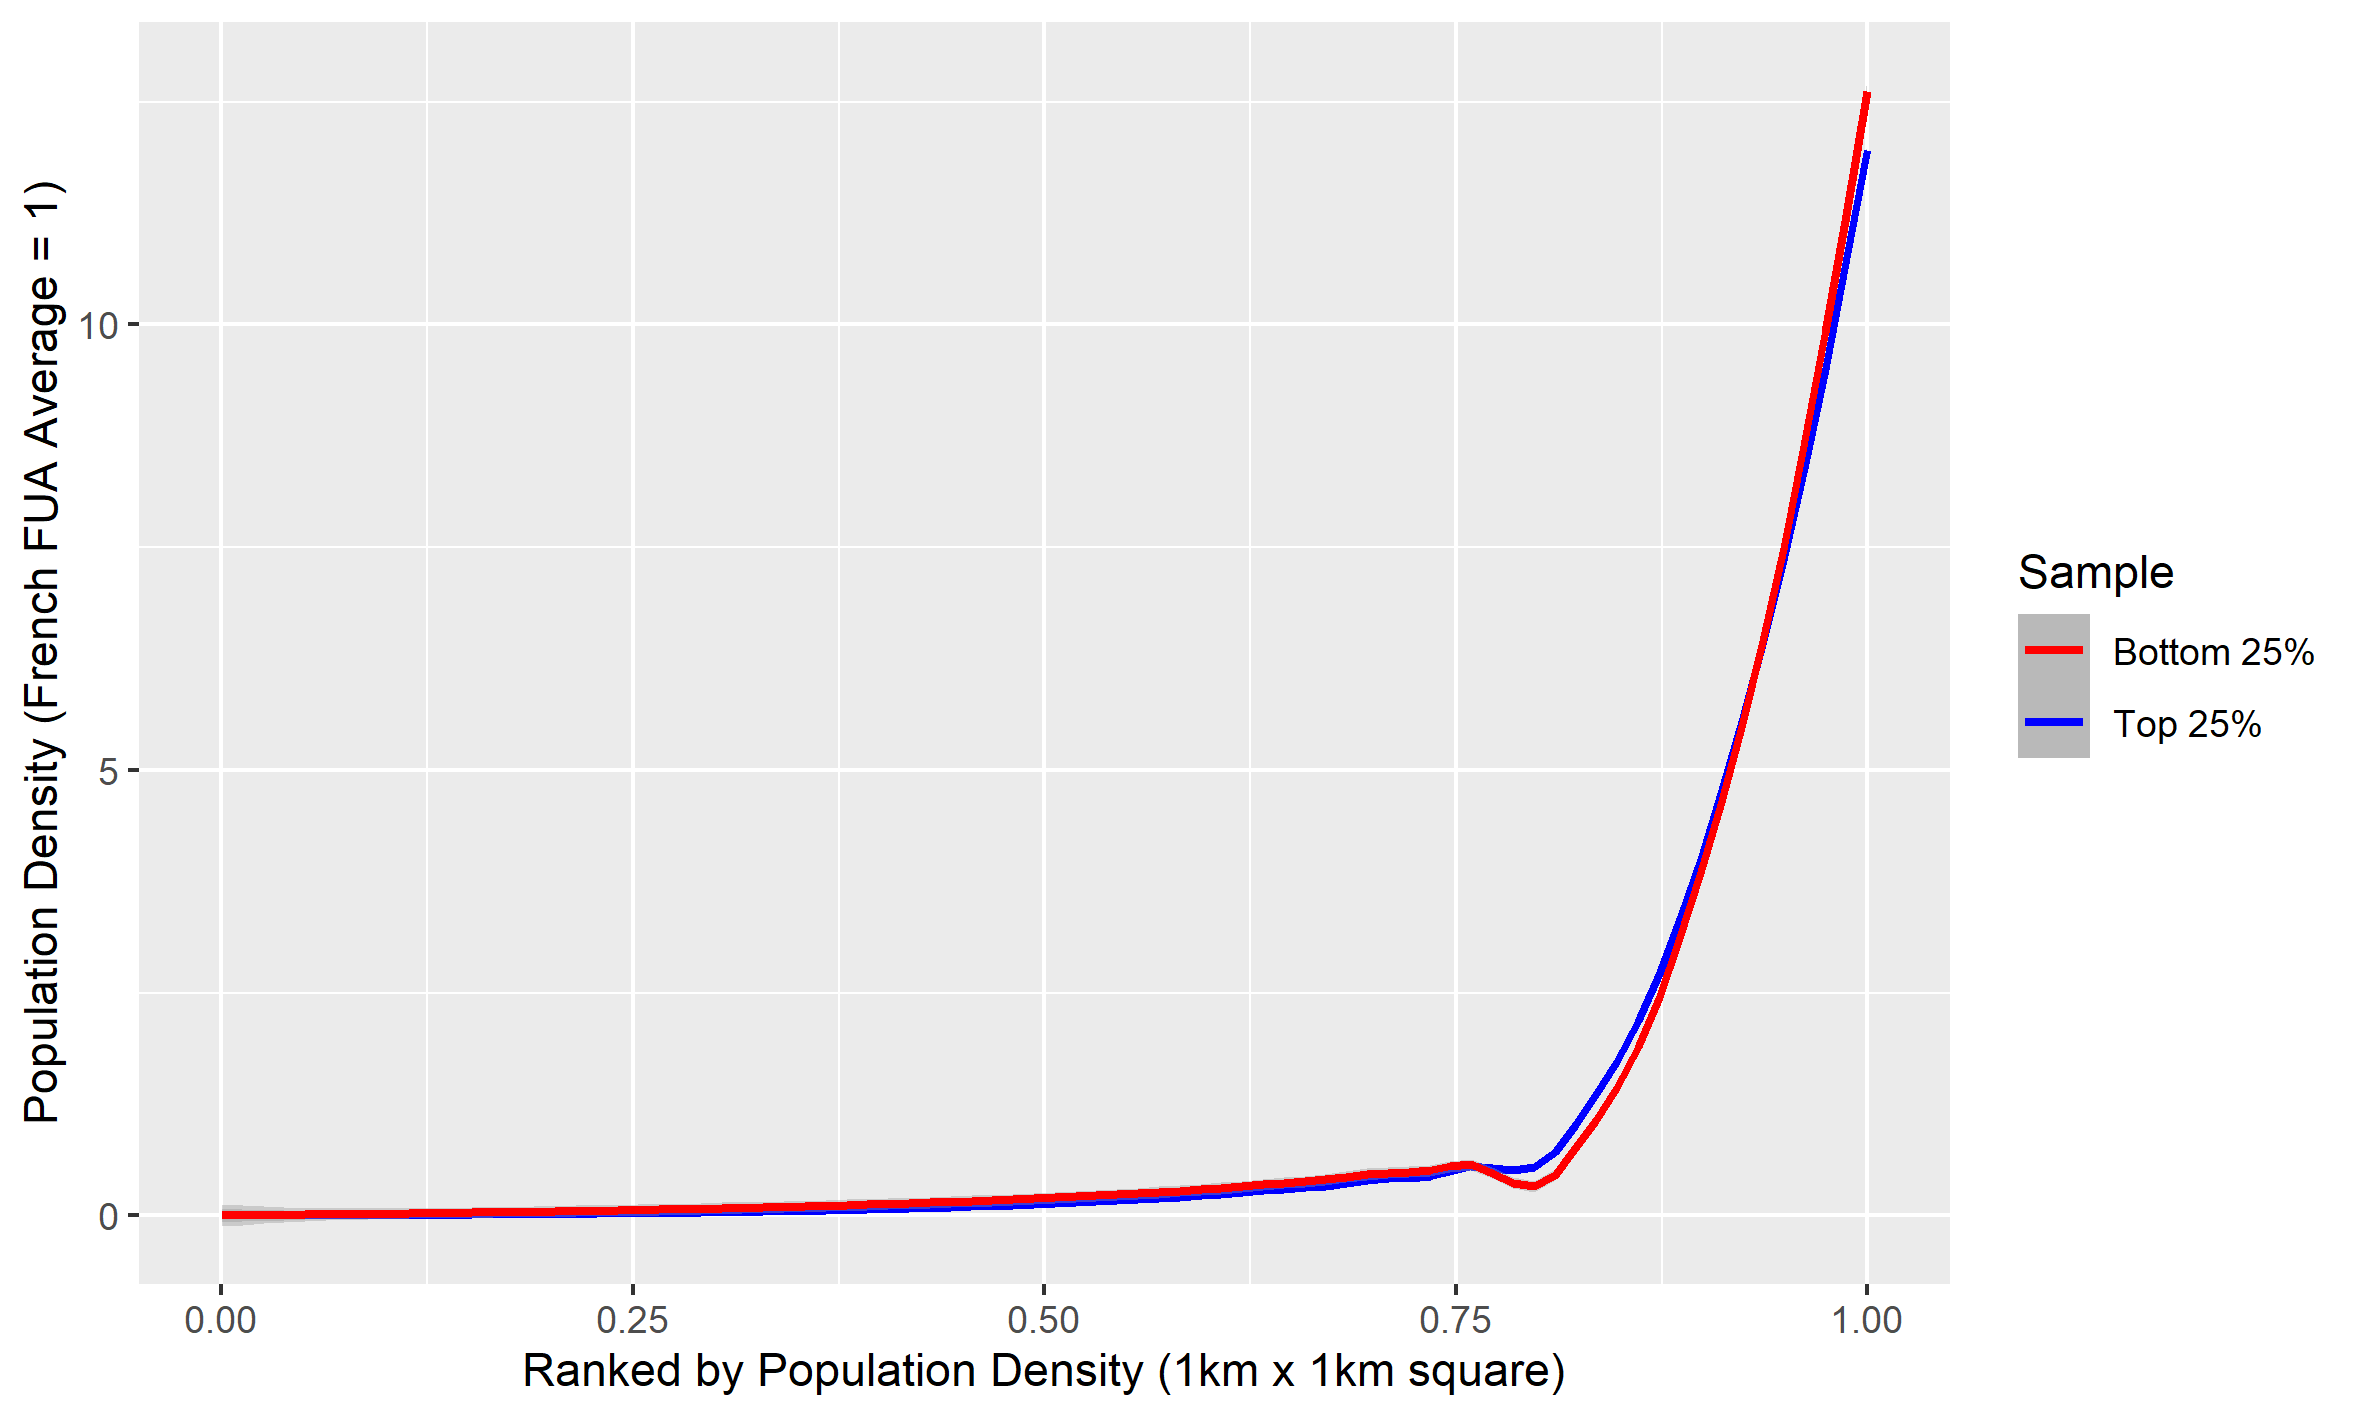
\includegraphics[width=\textwidth]{tractdens_dist_france.png}
		\caption{Loess regression with $\alpha = 0.5$. 95\% confidence intervals are reported}.\label{Dens_dist_france}
	\end{center}
\end{figure}


\subsection{1930 Census Data Construction}\label{1930CensusDFC}
Will be Completed
\begin{figure}[hbpt]
	\begin{center}
		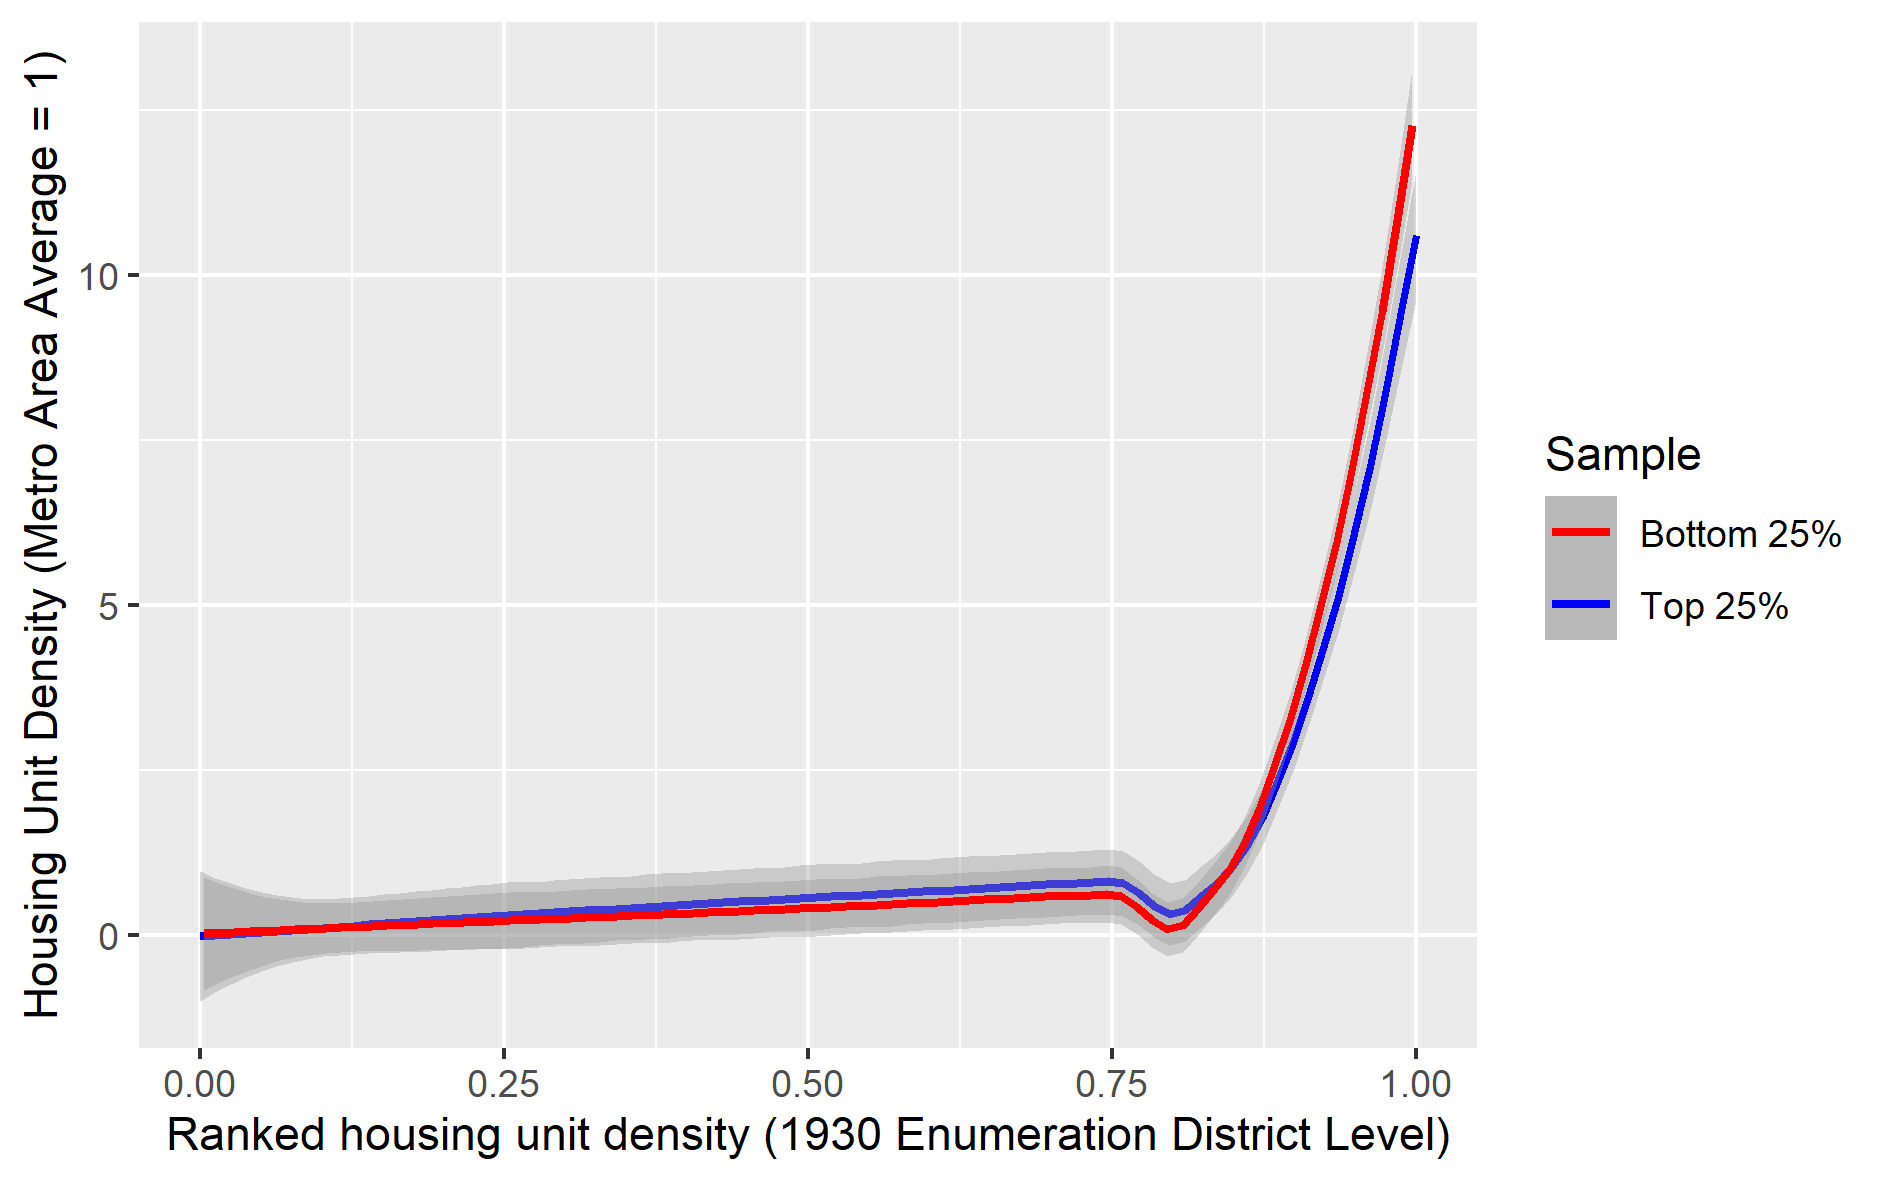
\includegraphics[width=\textwidth]{1930ED_dens_disp.png}
		\caption{Loess regression with $\alpha = 0.5$. 95\% confidence intervals are reported.}\label{Dens_dist_1930ED}
	\end{center}
\end{figure}


\newpage
\section{Appendix: Measuring Zoning Districts}\label{appendix:LotSize}

\begin{figure}[hbpt]
	\begin{center}
		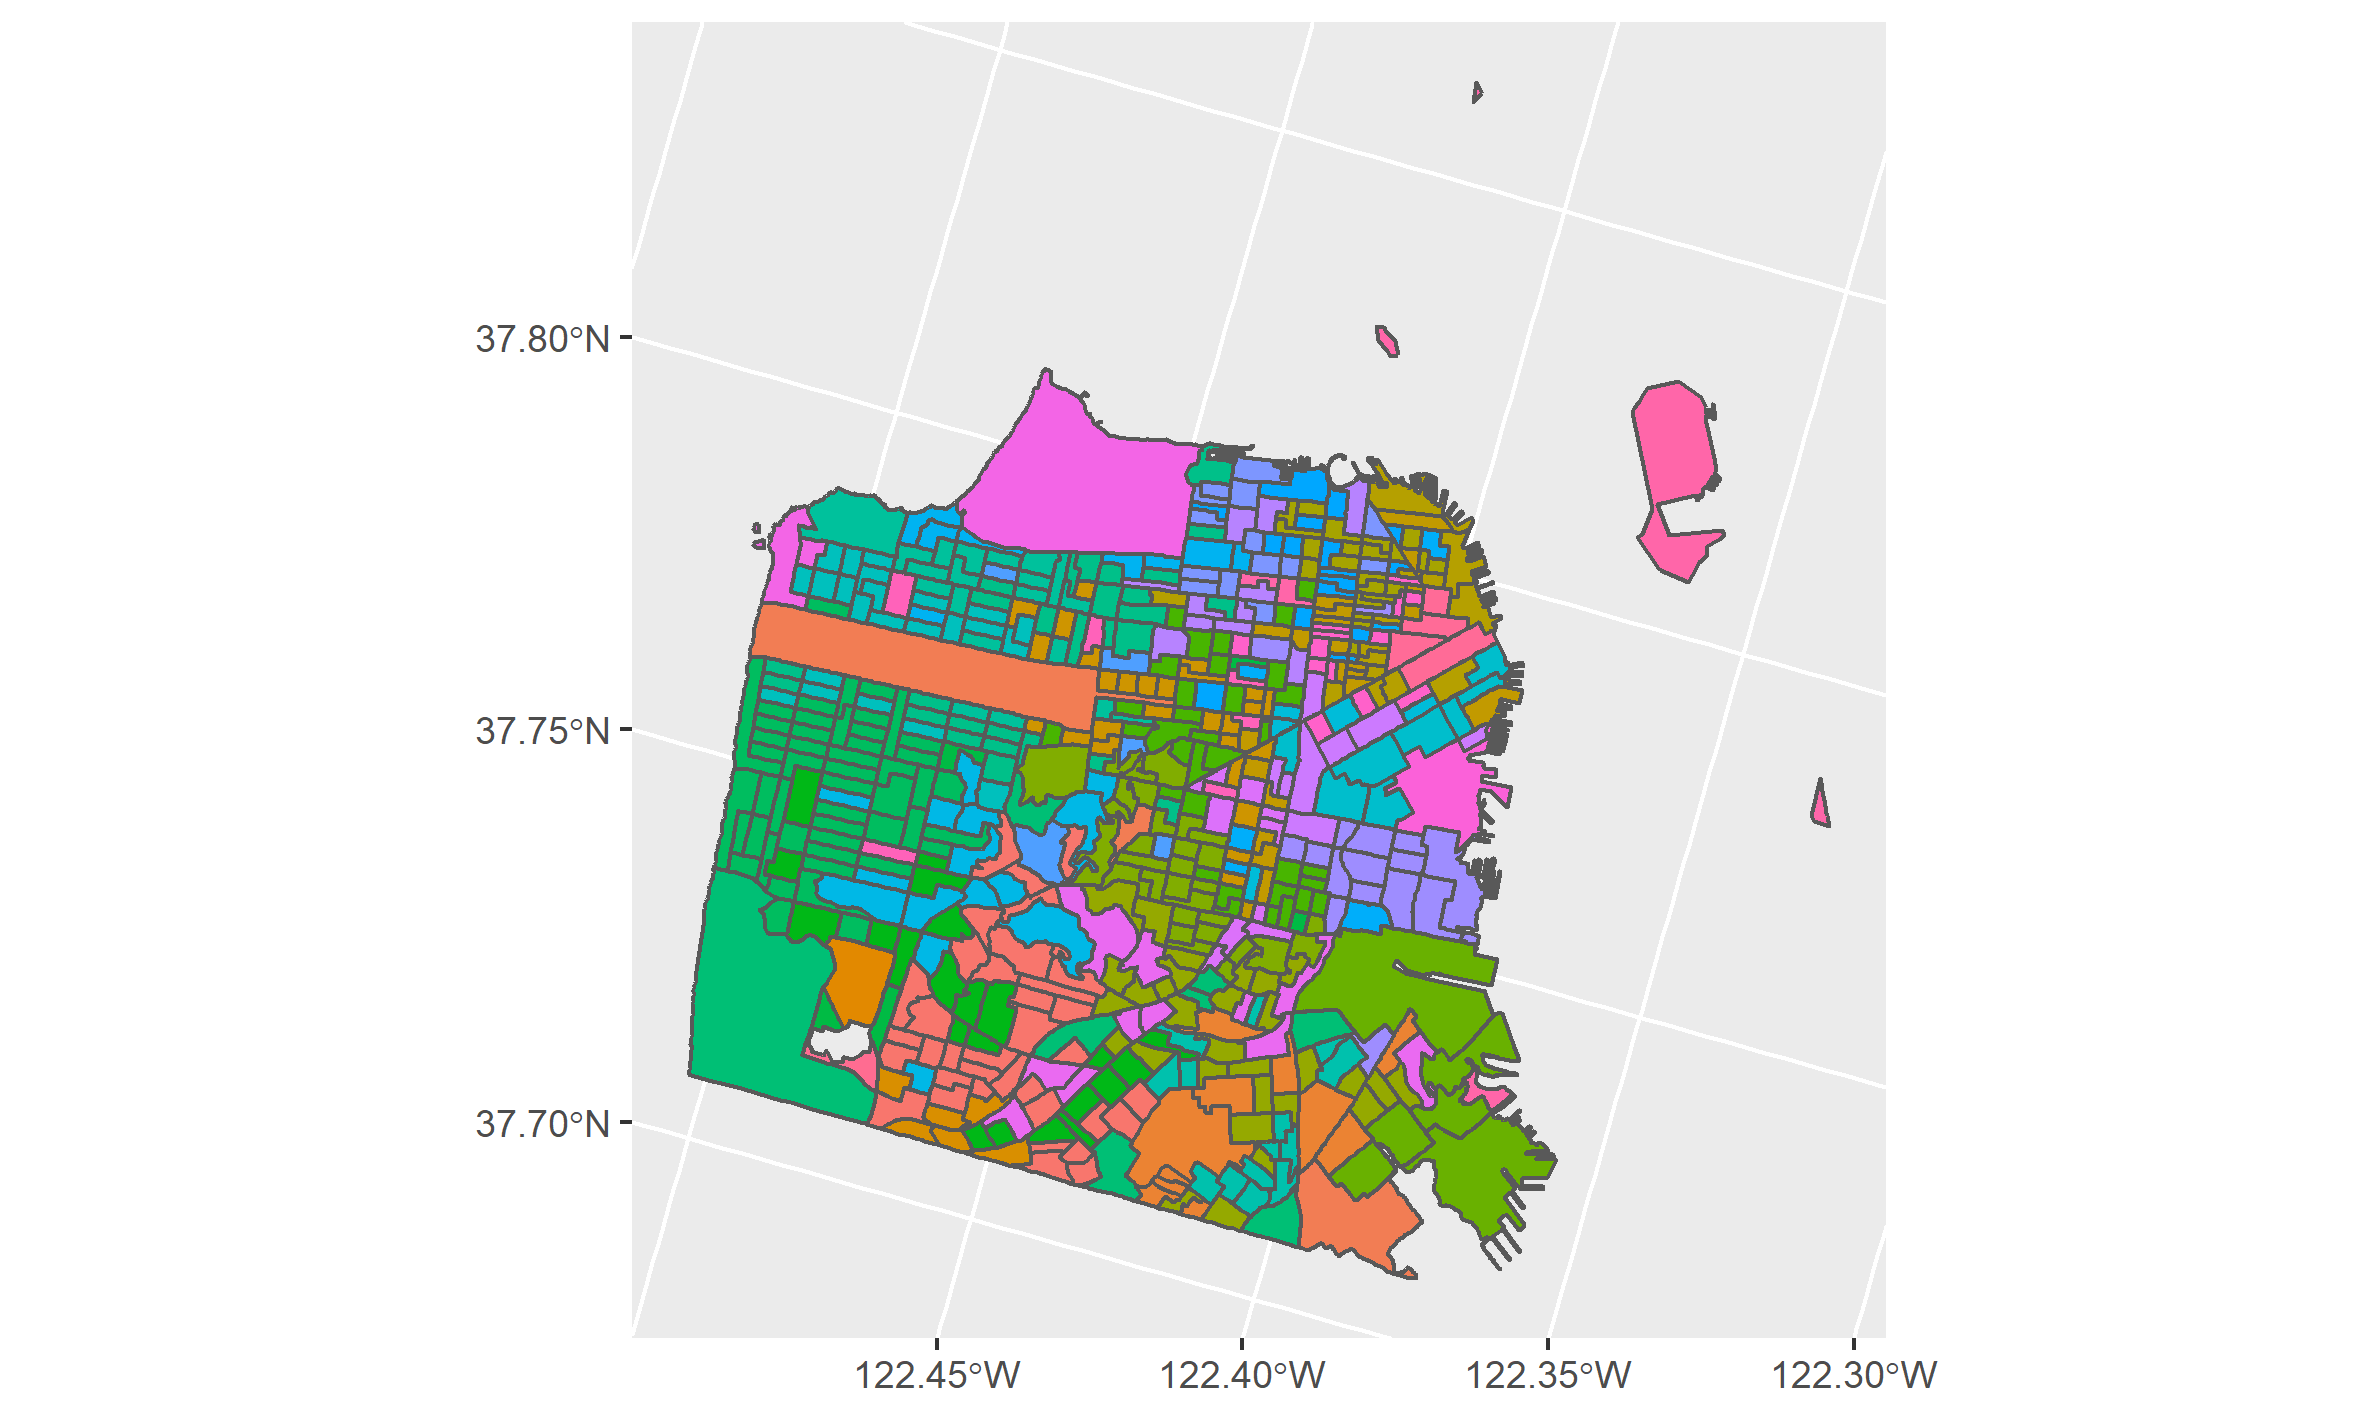
\includegraphics[width=\textwidth]{SF_MAP.png}

		\caption{41 Zoning Districts in San Francisco. While each district may not be a contiguous collection of block groups, the collection tend to be in close geographic proximity. }\label{ZoningDistrict}
	\end{center}
\end{figure}



\end{document}